%% 
%% Analysis 1&2 BSc, ETH
%%
%% (C) 2013 Sandro Felicioni
%% 
%% Partialy based on irgendeiner Zusammenfassung des Jahres 2012 by
%%	 - Gregor Wegberg
%%   - Leo Büttiker
%%   - Benjamin Steger
%%   - Philipp Küng
%%
%% Partialy based on "Analysis Zusammenfassung 2009" from Stefan Heule (http://summaries.stefanheule.com)
%%
%% License: Creative Commons Attribution-Share Alike 3.0 Unported
%% http://creativecommons.org/licenses/by-sa/3.0/
%% 


\documentclass[a4paper,titlepage,twocolumn]{article}
\usepackage[ngerman]{babel}

%%
%% 
%% (C) 2011 Gregor Wegberg
%%
%% Based on work of Stefan Heule, Licensed as Creative Commons Attribution-Share Alike 3.0 Unported
%% 
%% License: Creative Commons Attribution-Share Alike 3.0 Unported
%% http://creativecommons.org/licenses/by-sa/3.0/
%% 

%% The following lines need to be included in the main tex file
%\documentclass[portrait,a4paper,titlepage]{article}
%%%
%% 
%% (C) 2011 Gregor Wegberg
%%
%% Based on work of Stefan Heule, Licensed as Creative Commons Attribution-Share Alike 3.0 Unported
%% 
%% License: Creative Commons Attribution-Share Alike 3.0 Unported
%% http://creativecommons.org/licenses/by-sa/3.0/
%% 

%% The following lines need to be included in the main tex file
%\documentclass[portrait,a4paper,titlepage]{article}
%%%
%% 
%% (C) 2011 Gregor Wegberg
%%
%% Based on work of Stefan Heule, Licensed as Creative Commons Attribution-Share Alike 3.0 Unported
%% 
%% License: Creative Commons Attribution-Share Alike 3.0 Unported
%% http://creativecommons.org/licenses/by-sa/3.0/
%% 

%% The following lines need to be included in the main tex file
%\documentclass[portrait,a4paper,titlepage]{article}
%\input{standard-definitions.tex}

\usepackage[utf8]{inputenc}
\usepackage{fontenc}

\usepackage{color}
\usepackage{soul}
\usepackage{soulutf8}

% Stichwortverzeichnis
\usepackage{makeidx}
%\usepackage{idxlayout}

\usepackage{alltt}
\renewcommand{\ttdefault}{txtt}

\usepackage{amssymb,amsfonts,amsmath}
\usepackage[e]{esvect}

\usepackage{algorithmicx}

\usepackage[pdftex]{graphicx}
\usepackage{epstopdf}
\usepackage[svgnames]{xcolor}

\usepackage{cancel}

\usepackage{pgf,tikz}
\usetikzlibrary{arrows}

\usepackage{geometry}
\geometry{a4paper, left=20mm, right=20mm, top=25mm, bottom=20mm}

% Allows fancy stuff in the page header
\usepackage{fancyhdr}
\pagestyle{fancy}

% hyperref
\usepackage[colorlinks=false,pdfborder={0 0 0}]{hyperref}

% multirow and multicol
\usepackage{multirow}
\usepackage{multicol}
\columnsep24pt
\columnseprule0.1pt

% landscape
\usepackage{pdflscape}

% pbox for arbitrary box sizes
\usepackage{pbox}

% enumerate
\renewcommand\theenumi{\arabic{enumi}}
\renewcommand\labelenumi{\theenumi.}
\renewcommand\theenumii{\roman{enumii}}
\renewcommand\labelenumii{\theenumii)}

\usepackage{listings}
\lstset{
    floatplacement={tbp}
    basicstyle=\ttfamily\mdseries,
    identifierstyle=,
    stringstyle=\color{gray},
    numbers=left,
    numbersep=5pt,
    inputencoding=utf8,
    xleftmargin=8pt,
    xrightmargin=8pt,
    keywordstyle=[1]\bfseries,
    keywordstyle=[2]\bfseries,
    keywordstyle=[3]\bfseries,
    keywordstyle=[4]\bfseries,
    numberstyle=\tiny,
    stepnumber=1,
    breaklines=true,
    frame=lines,
    showstringspaces=false,
    tabsize=2,
    commentstyle=\color{gray},
    captionpos=b,
    float=float,
    language={Java}
}
\newcommand{\code}[1]{\lstinline{#1}}

% depth of section numbering
\setcounter{secnumdepth}{4}

%% Redefine the \paragraph command:
\makeatletter
\renewcommand{\paragraph}{\@startsection{paragraph}{4}{0mm}%
    {-\baselineskip}%
    {0.5\baselineskip}%
    {\normalfont\bfseries}%
}%
\makeatother

% parindent
\parindent0px
\parskip3pt

% redefine greek letters
\renewcommand{\phi}{\varphi}
\renewcommand{\epsilon}{\varepsilon}

% shortcuts in math mode
\newcommand{\bs}{\boldsymbol}
\newcommand{\mc}{\mathcal}
\newcommand{\norm}[1]{| \!\:\! | #1 | \!\:\! |}
\newcommand{\with}{\;|\;} % with in set notation
\newcommand{\ds}{\displaystyle}
\newcommand{\nop}[1]{}
\newcommand{\argmax}{\operatorname*{arg\;max}}
\newcommand{\argmin}{\operatorname*{arg\;min}}
\newcommand{\rmd}{\mathrm{d}} % for integrals
\newcommand{\ggT}{\operatorname*{ggT}}
\newcommand{\kgV}{\operatorname*{kgV}}
\newcommand{\id}{\operatorname{id}}
\newcommand{\grad}{\operatorname{grad}}
\newcommand{\rot}{\operatorname{rot}}
\newcommand{\arcsinh}{\operatorname{arcsinh}}
\newcommand{\arcosh}{\operatorname{arcosh}}
\newcommand{\arctanh}{\operatorname{arctanh}}

% shortcuts for comment below/above text/math
\newcommand{\comment}[2]{\overset{#1}{\overbrace{#2}}} % comment above term, requires amsmath
\newcommand{\ucomment}[2]{\underset{#1}{\underbrace{#2}}} % comment below term, requires amsmath
\newcommand{\commentt}[2]{$\overset{\text{#1}}{\overbrace{\text{#2}}}$} % comment above text, requires amsmath 

% number sets
\newcommand{\R}{\mathbb{R}}
\newcommand{\Z}{\mathbb{Z}}
\newcommand{\N}{\mathbb{N}}
\newcommand{\Q}{\mathbb{Q}}
\newcommand{\C}{\mathbb{C}}
\newcommand{\F}{\mathbb{F}}
\newcommand{\E}{\mathbb{E}}
\newcommand{\LL}{\mathcal{L}}
\newcommand{\powerset}{\mathcal P}

% probabilities
\newcommand{\Prob}[1]{\operatorname{Pr}\left[#1\right]}
\newcommand{\Ex}[1]{\mathbb{E}\left[#1\right]}

% todo
\newcommand{\todo}[1]{\sethlcolor{red}\hl{$\ggg$ \textbf{TODO} [#1]}\sethlcolor{yellow}}


% big-o notation
\newcommand{\bigO}[1]{\mc O\left(#1\right)}




\usepackage[utf8]{inputenc}
\usepackage{fontenc}

\usepackage{color}
\usepackage{soul}
\usepackage{soulutf8}

% Stichwortverzeichnis
\usepackage{makeidx}
%\usepackage{idxlayout}

\usepackage{alltt}
\renewcommand{\ttdefault}{txtt}

\usepackage{amssymb,amsfonts,amsmath}
\usepackage[e]{esvect}

\usepackage{algorithmicx}

\usepackage[pdftex]{graphicx}
\usepackage{epstopdf}
\usepackage[svgnames]{xcolor}

\usepackage{cancel}

\usepackage{pgf,tikz}
\usetikzlibrary{arrows}

\usepackage{geometry}
\geometry{a4paper, left=20mm, right=20mm, top=25mm, bottom=20mm}

% Allows fancy stuff in the page header
\usepackage{fancyhdr}
\pagestyle{fancy}

% hyperref
\usepackage[colorlinks=false,pdfborder={0 0 0}]{hyperref}

% multirow and multicol
\usepackage{multirow}
\usepackage{multicol}
\columnsep24pt
\columnseprule0.1pt

% landscape
\usepackage{pdflscape}

% pbox for arbitrary box sizes
\usepackage{pbox}

% enumerate
\renewcommand\theenumi{\arabic{enumi}}
\renewcommand\labelenumi{\theenumi.}
\renewcommand\theenumii{\roman{enumii}}
\renewcommand\labelenumii{\theenumii)}

\usepackage{listings}
\lstset{
    floatplacement={tbp}
    basicstyle=\ttfamily\mdseries,
    identifierstyle=,
    stringstyle=\color{gray},
    numbers=left,
    numbersep=5pt,
    inputencoding=utf8,
    xleftmargin=8pt,
    xrightmargin=8pt,
    keywordstyle=[1]\bfseries,
    keywordstyle=[2]\bfseries,
    keywordstyle=[3]\bfseries,
    keywordstyle=[4]\bfseries,
    numberstyle=\tiny,
    stepnumber=1,
    breaklines=true,
    frame=lines,
    showstringspaces=false,
    tabsize=2,
    commentstyle=\color{gray},
    captionpos=b,
    float=float,
    language={Java}
}
\newcommand{\code}[1]{\lstinline{#1}}

% depth of section numbering
\setcounter{secnumdepth}{4}

%% Redefine the \paragraph command:
\makeatletter
\renewcommand{\paragraph}{\@startsection{paragraph}{4}{0mm}%
    {-\baselineskip}%
    {0.5\baselineskip}%
    {\normalfont\bfseries}%
}%
\makeatother

% parindent
\parindent0px
\parskip3pt

% redefine greek letters
\renewcommand{\phi}{\varphi}
\renewcommand{\epsilon}{\varepsilon}

% shortcuts in math mode
\newcommand{\bs}{\boldsymbol}
\newcommand{\mc}{\mathcal}
\newcommand{\norm}[1]{| \!\:\! | #1 | \!\:\! |}
\newcommand{\with}{\;|\;} % with in set notation
\newcommand{\ds}{\displaystyle}
\newcommand{\nop}[1]{}
\newcommand{\argmax}{\operatorname*{arg\;max}}
\newcommand{\argmin}{\operatorname*{arg\;min}}
\newcommand{\rmd}{\mathrm{d}} % for integrals
\newcommand{\ggT}{\operatorname*{ggT}}
\newcommand{\kgV}{\operatorname*{kgV}}
\newcommand{\id}{\operatorname{id}}
\newcommand{\grad}{\operatorname{grad}}
\newcommand{\rot}{\operatorname{rot}}
\newcommand{\arcsinh}{\operatorname{arcsinh}}
\newcommand{\arcosh}{\operatorname{arcosh}}
\newcommand{\arctanh}{\operatorname{arctanh}}

% shortcuts for comment below/above text/math
\newcommand{\comment}[2]{\overset{#1}{\overbrace{#2}}} % comment above term, requires amsmath
\newcommand{\ucomment}[2]{\underset{#1}{\underbrace{#2}}} % comment below term, requires amsmath
\newcommand{\commentt}[2]{$\overset{\text{#1}}{\overbrace{\text{#2}}}$} % comment above text, requires amsmath 

% number sets
\newcommand{\R}{\mathbb{R}}
\newcommand{\Z}{\mathbb{Z}}
\newcommand{\N}{\mathbb{N}}
\newcommand{\Q}{\mathbb{Q}}
\newcommand{\C}{\mathbb{C}}
\newcommand{\F}{\mathbb{F}}
\newcommand{\E}{\mathbb{E}}
\newcommand{\LL}{\mathcal{L}}
\newcommand{\powerset}{\mathcal P}

% probabilities
\newcommand{\Prob}[1]{\operatorname{Pr}\left[#1\right]}
\newcommand{\Ex}[1]{\mathbb{E}\left[#1\right]}

% todo
\newcommand{\todo}[1]{\sethlcolor{red}\hl{$\ggg$ \textbf{TODO} [#1]}\sethlcolor{yellow}}


% big-o notation
\newcommand{\bigO}[1]{\mc O\left(#1\right)}




\usepackage[utf8]{inputenc}
\usepackage{fontenc}

\usepackage{color}
\usepackage{soul}
\usepackage{soulutf8}

% Stichwortverzeichnis
\usepackage{makeidx}
%\usepackage{idxlayout}

\usepackage{alltt}
\renewcommand{\ttdefault}{txtt}

\usepackage{amssymb,amsfonts,amsmath}
\usepackage[e]{esvect}

\usepackage{algorithmicx}

\usepackage[pdftex]{graphicx}
\usepackage{epstopdf}
\usepackage[svgnames]{xcolor}

\usepackage{cancel}

\usepackage{pgf,tikz}
\usetikzlibrary{arrows}

\usepackage{geometry}
\geometry{a4paper, left=20mm, right=20mm, top=25mm, bottom=20mm}

% Allows fancy stuff in the page header
\usepackage{fancyhdr}
\pagestyle{fancy}

% hyperref
\usepackage[colorlinks=false,pdfborder={0 0 0}]{hyperref}

% multirow and multicol
\usepackage{multirow}
\usepackage{multicol}
\columnsep24pt
\columnseprule0.1pt

% landscape
\usepackage{pdflscape}

% pbox for arbitrary box sizes
\usepackage{pbox}

% enumerate
\renewcommand\theenumi{\arabic{enumi}}
\renewcommand\labelenumi{\theenumi.}
\renewcommand\theenumii{\roman{enumii}}
\renewcommand\labelenumii{\theenumii)}

\usepackage{listings}
\lstset{
    floatplacement={tbp}
    basicstyle=\ttfamily\mdseries,
    identifierstyle=,
    stringstyle=\color{gray},
    numbers=left,
    numbersep=5pt,
    inputencoding=utf8,
    xleftmargin=8pt,
    xrightmargin=8pt,
    keywordstyle=[1]\bfseries,
    keywordstyle=[2]\bfseries,
    keywordstyle=[3]\bfseries,
    keywordstyle=[4]\bfseries,
    numberstyle=\tiny,
    stepnumber=1,
    breaklines=true,
    frame=lines,
    showstringspaces=false,
    tabsize=2,
    commentstyle=\color{gray},
    captionpos=b,
    float=float,
    language={Java}
}
\newcommand{\code}[1]{\lstinline{#1}}

% depth of section numbering
\setcounter{secnumdepth}{4}

%% Redefine the \paragraph command:
\makeatletter
\renewcommand{\paragraph}{\@startsection{paragraph}{4}{0mm}%
    {-\baselineskip}%
    {0.5\baselineskip}%
    {\normalfont\bfseries}%
}%
\makeatother

% parindent
\parindent0px
\parskip3pt

% redefine greek letters
\renewcommand{\phi}{\varphi}
\renewcommand{\epsilon}{\varepsilon}

% shortcuts in math mode
\newcommand{\bs}{\boldsymbol}
\newcommand{\mc}{\mathcal}
\newcommand{\norm}[1]{| \!\:\! | #1 | \!\:\! |}
\newcommand{\with}{\;|\;} % with in set notation
\newcommand{\ds}{\displaystyle}
\newcommand{\nop}[1]{}
\newcommand{\argmax}{\operatorname*{arg\;max}}
\newcommand{\argmin}{\operatorname*{arg\;min}}
\newcommand{\rmd}{\mathrm{d}} % for integrals
\newcommand{\ggT}{\operatorname*{ggT}}
\newcommand{\kgV}{\operatorname*{kgV}}
\newcommand{\id}{\operatorname{id}}
\newcommand{\grad}{\operatorname{grad}}
\newcommand{\rot}{\operatorname{rot}}
\newcommand{\arcsinh}{\operatorname{arcsinh}}
\newcommand{\arcosh}{\operatorname{arcosh}}
\newcommand{\arctanh}{\operatorname{arctanh}}

% shortcuts for comment below/above text/math
\newcommand{\comment}[2]{\overset{#1}{\overbrace{#2}}} % comment above term, requires amsmath
\newcommand{\ucomment}[2]{\underset{#1}{\underbrace{#2}}} % comment below term, requires amsmath
\newcommand{\commentt}[2]{$\overset{\text{#1}}{\overbrace{\text{#2}}}$} % comment above text, requires amsmath 

% number sets
\newcommand{\R}{\mathbb{R}}
\newcommand{\Z}{\mathbb{Z}}
\newcommand{\N}{\mathbb{N}}
\newcommand{\Q}{\mathbb{Q}}
\newcommand{\C}{\mathbb{C}}
\newcommand{\F}{\mathbb{F}}
\newcommand{\E}{\mathbb{E}}
\newcommand{\LL}{\mathcal{L}}
\newcommand{\powerset}{\mathcal P}

% probabilities
\newcommand{\Prob}[1]{\operatorname{Pr}\left[#1\right]}
\newcommand{\Ex}[1]{\mathbb{E}\left[#1\right]}

% todo
\newcommand{\todo}[1]{\sethlcolor{red}\hl{$\ggg$ \textbf{TODO} [#1]}\sethlcolor{yellow}}


% big-o notation
\newcommand{\bigO}[1]{\mc O\left(#1\right)}



\usepackage{geometry}
\usepackage{amsthm}
\usepackage{enumitem}

\setlist{nolistsep}

\geometry{top=1cm, headsep=0pt,headheight=0.5cm, % top part
bottom=1cm, footskip=0.5cm, % bottom part
left=0.4cm,right=0.4cm} % left / right part

% fancy header
\renewcommand{\footrulewidth}{0pt}
\renewcommand{\headrulewidth}{0pt}
\renewcommand{\headwidth}{\textwidth}

\tabcolsep=0.1cm

% Redefine section commands to use less space
\makeatletter
\renewcommand{\section}{\@startsection{section}{1}{0mm}%
                                {-1ex plus -.5ex minus -.2ex}%
                                {0.5ex plus .2ex}%x
                                {\normalfont\large\bfseries}}
\renewcommand{\subsection}{\@startsection{subsection}{2}{0mm}%
                                {-1explus -.5ex minus -.2ex}%
                                {0.5ex plus .2ex}%
                                {\normalfont\normalsize\bfseries}}
\renewcommand{\subsubsection}{\@startsection{subsubsection}{3}{0mm}%
                                {-1ex plus -.5ex minus -.2ex}%
                                {1ex plus .2ex}%
                                {\normalfont\small\bfseries}}
\makeatother

\usepackage{amsthm}

\theoremstyle{plain}
\newtheorem{lemma}{Lemma}[section]
\newtheorem{theorem}{Theorem}[section]
\newtheorem{corollary}{Korollar}[section]
\newtheorem{tipp}{Tipp}[section]

\theoremstyle{definition}
\newtheorem{definition}{Definition}[section]
\newtheorem{satz}{Satz}[section]
\newtheorem{hilfssatz}{Hilfssatz}[section]


\graphicspath{{./data/}}

\usepackage{empheq}

\makeindex

\begin{document}
% remove not needed whitespace
\setlength{\jot}{0pt}
\setlength{\abovedisplayskip}{0pt}
\setlength{\abovedisplayshortskip}{0pt}
\setlength{\belowdisplayskip}{0pt} 
\setlength{\belowdisplayshortskip}{0pt}

\onecolumn
{\footnotesize
\begin{multicols}{3}
\thispagestyle{empty}
\setcounter{tocdepth}{3}
\tableofcontents
\end{multicols}

%\idxlayout{columns=4,rule=0.1pt}
%\printindex
}
\twocolumn
\newpage
\setcounter{page}{1}
\pagestyle{plain}

\section{Vollständige Induktion}\index{Induktion}
Grundlegende Struktur um die Aussage $A(n)$ zu beweisen:
\begin{enumerate}
	\item \textbf{Verankerung/Induktionsanfang:} Die Aussage wird für $n = A$ bewiesen.
	$A$ ist dabei meistens der erste Wert für die gegebene Eingabemenge.
	Der Beweis wird meist durch direktes ausrechnen gemacht.
	\item \textbf{Annahme/Induktionsvoraussetzung:} Hier schreibt man,
	dass man davon ausgeht die Aussage sei gültig für ein bestimmtes $n \in \N$ (damit man sie im 4. Schritt
	einsetzen kann). Man kopiert also im Grunde, was man zu beweisen hat mit einigen Zierwörter.
	\item \textbf{Induktionsbehauptung:} Hier schreibt man, dass die Aussage auch für (n + 1) gilt.
	\item \textbf{Induktionsschritt:} Hier beweist man, dass unter der Annahme, dass die Induktionsvoraussetzung gilt, die Induktionsbehauptung folgt. Oder anders gesagt, wir beweisen dass wenn die Aussage für n gilt, dass es dann auch für (n + 1) gelten muss. Dazu wird die Induktionsannahme verwendet.
\end{enumerate}
Merke: Schritt 2 und 3 werden oft weggelassen, wenn zu trivial!\\
\textbf{Beispiel}\\
Es ist zu beweisen, dass für jedes $n \in \N$ folgendes gilt:\\
$1 + 2 + 3 + \ldots + n = \frac{n(n + 1)}{2}$
\begin{enumerate}
	\item \textbf{Verankerung:} Für $n = 1$ gilt: $1 = \frac{1 (1 + 1)}{2} = \frac{2}{2} = 1 \quad \checkmark$ 
	\item \textbf{Annahme:} $1 + 2 + 3 + \ldots + n = \frac{n(n+1)}{2}, \; \text{für ein} \; n \in \N$
	\item \textbf{Induktionsbehauptung:} Wenn die Aussage für n gilt, dann gilt sie auch für (n + 1).
	\item \textbf{Induktionsschritt:} Für $n \to n+1$ gilt:
	\begin{align*}
	1 + 2 + \ldots + n + (n+1) \overset{\text{Annahme}}{=} & \frac{n(n+1)}{2} + (n + 1)\\
	&= \frac{n(n+1)}{2} + \frac{2n + 2}{2} \\
	&= \frac{n^2 + n + 2n + 2}{2} \\
	&= \frac{(n + 1)(n + 2)}{2} _\square
	\end{align*}
\end{enumerate}
\section{Logik}\index{Logik}
\subsection{Aussagenlogik}
Seien A und B zwei Aussagen die wahr oder falsch sein können.
\begin{itemize}
	\item A ist eine \textbf{notwendige Bedingung} für B. \\
	Dh: B kann ohne A nicht erfüllbar sein oder anders, wenn B erfüllt ist dann muss A auch zwingend erfüllt sein. \\
	Also: $B \Rightarrow A$

	\item A ist eine \textbf{hinreichende Bedingung} für B. \\
	Dh: Wenn A erfüllt ist, ist auch sicher B erfüllt. \\
	Also: $A \Rightarrow B$

	\item A ist eine \textbf{notw.} und \textbf{hinreichende Bedingung} für B.\\
	Dh: A ist genau dann erfüllt wenn auch B erfüllt ist\small{(en: iff)}\\
	Also: $A \Leftrightarrow B$ oder $(B \Rightarrow A \wedge A \Rightarrow B)$
\end{itemize}

\subsection{Logische Symbole}
{\footnotesize
\begin{tabular}{|c|l|c|}\hline
	\textbf{Symbol} & \textbf{Bedeutung} & \textbf{Beweis von solchen Aussagen}\\\hline
	$A \Leftrightarrow B$ & genau dann, wenn & \pbox{2cm}{$A \Rightarrow B$ \\ $B \Rightarrow A$} oder \pbox{2cm}{$A \Rightarrow B$ \\ $\neg A \Rightarrow \neg B$} \\\hline
	$A \Rightarrow B$ & impliziert / wenn dann & \pbox{4cm}{$A \Rightarrow B$ oder $\neg B \Rightarrow \neg A$ oder\\$(A \wedge \neg B)$ Diese Annahme zum Widerspruch führen}\\
	\hline
\end{tabular}
}
\section{Mengen}\index{Menge}

\subsection{Definitionen}\label{sec:mengen-def}
{\footnotesize
\begin{tabular}{|l|l|l|}\hline
	\textbf{Name} & \textbf{Mengensymbol} & \textbf{Definition} \\ \hline
	\textbf{Teilmenge:} & $A \subseteq B$ & $\forall x: x \in A \rightarrow x \in B$ \\
	\textbf{Vereinigung:} & $A \cup B$ & $ \{x \,|\, x \in A \lor x \in B\}$ \\
	\textbf{Durchschnitt:} & $A \cap B$ & $ \{x \,|\, x \in A \land x \in B\}$ \\
	\textbf{Differenz:} & $A \backslash B = A - B $ & $ \{x \,|\, x \in A \land x \not\in B\}$ \\
	\textbf{Komplement:} & $A^c = \overline{A} $ & $ \{x \,|\, x \not\in A\}$ \\
	\hline
\end{tabular}
}

\subsection{Rechenregeln}
{\footnotesize
\begin{tabular}{|l|r|}\hline
$A \cup B = B \cup A$ & $A \cap B = B \cap A$\\
$A \cup (B \cup C) = (A \cup B) \cup C$ & $A \cap (B \cap C) = (A \cap B) \cap C$\\
$A \cup (B \cap C) = (A \cup B) \cap (A \cup C)$ & $A \cap (B \cup C) = (A \cap B) \cup (A \cap C)$\\
$(A \cup B)^c = A^c \cap B^c$ & $(A \cap B)^c = A^c \cup B^c$\\
$(A \backslash B) \cup C = (A \cup C) \cap (B^c \cup C)$ & $(A \backslash B) \cap C = A \backslash )(B \cup C^c)$\\
$(A \backslash B) \backslash C = A \backslash (B \cup C)$ & $A \backslash B = A \cap B^c$\\\hline
\end{tabular}
}

\subsection{Beweise}
Um Mengengleichungen zu beweisen überführt man üblicherweise eine Seite in eine Form,
die nur noch aus logischen Operatoren besteht ($\land, \lor, \in, \not\in$) und formt
dann so um, dass man zur gewünschten anderen Seite kommt durch Rückführung in eine
Form mit Mengenoperatoren. Dazu verwendet man am einfachsten die Definitionen in Sektion \ref{sec:mengen-def}.

\subsection*{Beispiel}
Zeige: $(A \cup B)^c = A^c \cap B^c$ wobei $A, B$ Untermengen von $X$ sind.
\begin{align*}
(A \cup B)^c &= \{x \in X: x \not\in (A \cup B)\} = \{x \in X: x \not\in A \land x \not\in B\}\\
&= \{x \in X: x \not\in A\} \cap \{x \in X: x \not\in B\} = A^c \cap B^c
\end{align*}

\subsection{bekannte Mengen}
\begin{description}
	\item[$\N$, natürliche Zahlen:] $\{1, 2, 3, \ldots\}$
	\item[$\Z$, ganze Zahlen:] $\{\ldots, -3, -2, -1, 0, 1, 2, 3, \ldots\}$
	\item[$\Q$, rationale Zahlen:] $\{\frac{p}{q} | p \in \Z, q \in \N \backslash \{0\}\}$
	\item[$\R$, reelle Zahlen:] rationale und irrationalen Zahlen.
\end{description}

\subsection{Mächtigkeit}\index{Mächtigkeit}
Eine Menge $A$ ist gleichmächtig zu einer Menge $B$, wenn es eine \textit{Bijektion}
$f: A \rightarrow B$ gibt. Man schreibt dann $|A| = |B|$.

Hat man zwischen zwei Mengen eine Funktion $f: A \rightarrow B$ gefunden, die bijektiv ist,
so gibt es eine Umkehrfunktion, die ebenfalls Bijektiv ist. Diese bildet jedes Element von $B$
auf eines aus $A$ ab.

\subsubsection{Abzählbar}\index{abzählbar}
Eine Menge $A$ ist abzählbar, wenn sie gleichmächtig zur Menge $\N$ (natürliche Zahlen) ist.

\subsubsection{Gleichmächtigkeit zeigen}
Zeigt man durch angeben einer bijektiven Funktion.

\textbf{Beispiel:}
Zeige: $U := \{ 2k + 1: k \in \N \}$ ist gleichmächtig zu $\N$.

\textbf{Beweis}: Sei $f: \N \rightarrow U$ gegeben durch
\begin{equation*}
f(n) = \left\{
	\begin{array}{l l}
		n & n \text{ ungerade}\\
		-n - 1 & n \text{ gerade}
	\end{array}
\right.
\end{equation*}

Diese Funktion ist offensichtlich bijektiv (sonst Umkehrfunktion angeben), wodurch $U$ gleichmächtig $\N$ ist.

\subsubsection{weitere gleichmächtige Mengen}
\begin{itemize}
	\item $\N, \Z, \Q$ sind gleichmächtig
	\item $\R, ]0,1[$ sind gleichmächtig
	\item $\R$ ist mächtiger (``überabzählbar'') als $\N$
\end{itemize}

\subsection{Teilmengen von $\R$}
\subsubsection{Intervalle}\index{Intervall}
\begin{tabular}{|l|l|l|}\hline
Schreibweise & Definition & Bezeichnung des Intervalls\\\hline
$]a, b[, (a,b)$ & $\{x \in \R | a < x < b\}$ & offen\\\hline
$[a, b[, [a, b)$ & $\{x \in \R | a \leq x < b\}$ & (rechts) halboffen \\\hline
$]a,b], (a, b]$ & $\{x \in \R | a < x \leq b\}$ & (links) halboffen \\\hline
$[a,b]$ & $\{x \in \R | a \leq x \leq b\}$ & abgeschlossen \\\hline
\end{tabular}

Achtung: Ist $a$ oder $b$ ``unendlich'' ($\pm \infty$), so muss es auf der entsprechenden Seite offen sein: z.B. $[a, $\hl{$\infty[$}, \hl{$]-\infty$}$, b[$.
Unendlich ist keine konkrete Zahl und kann somit nicht gleich einer anderen Zahl sein, was nötig wäre für $\leq$.
\pagebreak

\begin{description}
	\item [Abgeschlossene Menge:] Eine Menge ist abgeschlossen, wenn ihr Komplement eine offene Menge ist. Bsp. Alle abgeschlossenen Intervalle (z.B: $[0, 1]$ da $(-\infty, 0) \cup (1, \infty)$)

	\item [Offene Menge:] Anschaulich ist eine Menge offen, wenn kein Element der Menge auf ihrem Rand liegt. Bsp. Alle offenen Intervale (z.B: $(0, 1)$ da $0,1 \notin (0, 1)$)

	\item [Kompakte Menge:] Eine Menge ist kompakt, wenn sie abgeschlossen und beschränkt ist! Bsp. Alle abgeschlossenen Intervalle (z.B: $[0, 1]$ da abgeschlossen und beschränkt)
\end{description}
Merke: Halboffene Mengen sind weder offen noch abgeschlossen.

\subsubsection{Beschränktheit}\index{beschränkt}
Eine nichtleere Teilmenge $M \subset \R$ heisst \underline{beschränkt}, falls es ein $C_1, C_2 \in \R$ gibt, sodass 
$\forall x \in M: C_1 \leq x \leq C_2$\\
(Alternativ: $\exists C \in \R \; \forall x \in M: |x| \leq C$)

\vspace{2pt}Eine nichtleere Teilmenge $M \subset \R$ heisst \underline{nach oben beschränkt}, falls 
$\exists C \in \R \; \forall x \in M: x \leq C$ \hspace{2pt} {\scriptsize(jedes derartige C heisst obere Schranke)}

\vspace{2pt}Eine nichtleere Teilmenge $M \subset \R$ heisst \underline{nach unten beschränkt}, falls 
$\exists C \in \R \; \forall x \in M: C \leq x$ \hspace{2pt} {\scriptsize(jedes derartige C heisst untere Schranke)}

\subsubsection{Supremum / Infimum}\index{Supremum}\index{Infimum}\index{Schranke}
Jede nach oben beschränkte Menge $M \subset \R$ besitzt eine kleinste obere Schranke $c = \sup \, M$ und nennt es \underline{Supremum von M}.

Jede nach unten beschränkte Menge $M \subset \R$ besitzt eine grösste untere Schranke $\tilde{c} = \inf \, M$ und nennt es \underline{Infimum von M}.


Falls die Menge $M$ ein grösstes (bzw. kleinstes) Element besitzt, so nennt man es \underline{Maximum} (bzw. \underline{Minimum}).
Es gilt:
\begin{itemize}
	\item Ist $M \subset \R$ abgeschlossen und beschränkt, so existieren Minimum und Maximum von $M$
	\item Wenn $\max M$ existiert, dann ist $\sup M = \max M$
	\item Ist $\sup M \in M$, so ist $\max M = \sup M$
	\item Wenn $\min M$ existiert, dann ist $\inf M = \min M$
	\item Ist $\inf M \in M$, so ist $\min M = \inf M$
\end{itemize}

\paragraph{mathematische Definition}
$\sup M = a$ gilt genau dann, wenn
\begin{itemize}
	\item $\forall x \in M: x \leq a$, $a$ ist somit obere Schranke von $M$
	\item $\forall \epsilon > 0 \; \exists x \in M: x > a - \epsilon$, d.h. $a - \epsilon$ ist keine obere Schranke mehr, egal wie klein man $\epsilon$ auch wählt $\rightarrow$ $a$ ist kleinste obere Schranke.
\end{itemize}

$\inf M = a$ gilt genau dann, wenn
\begin{itemize}
	\item $\forall x \in M: x \geq a$, $a$ ist somit untere Schranke von $M$
	\item $\forall \epsilon > 0 \; \exists x \in M: x < a + \epsilon$, d.h. $a + \epsilon$ ist keine untere Schranke mehr, egal wie klein man $\epsilon$ auch wählt $\rightarrow$ $a$ ist grösste untere Schranke.
\end{itemize}

\subsubsection{Maximum / Minimum} \index{Maximum / Minimum}
\begin{satz}[Extremwertsatz - Weierstrass] Ist f eine stetige Funktion und ist der Definitionsbereich kompakt (Bsp. abgeschlossenes Intervall), so hat die Funktion ein Maximum und Minimum.
\end{satz}
\textbf{Tip:} Wenn Max/Min bestummen werden soll, prüfe zuerst ob f stetig ist auf ganzem Definitionsberech (beachte Übergang bei Fallunterscheidungen) und ob Definitionsbereich kompakt ist!

\subsubsection{Archimedisches Prinzip}\index{archimedisches Prinzip}
\begin{satz}[Archimedisches Prinzip]
Zu den zwei Zahlen $x, y \in \R, \; y > x > 0$ existiert eine Zahl $n \in \N$, sd gilt: $nx > y$
\end{satz}
\vspace{-0.1cm}
Geometrisch: Hat man zwei Strecken auf einer Geraden, so kann man die grössere von beiden übertreffen, wenn man die kleinere nur oft genug abträgt.
\pagebreak

\section{Funktionen}
Eine Funktion $f: D \rightarrow W$ ist eine Abbildung, in der jedes Element aus
$D$ einem Element aus $W$ zugeordnet wird. $D$ ist der \underline{Definitionsbereich}
(Bereich der gültigen Eingaben) und $W$ der \underline{Wertebereich}
(Bereich der gültigen Ausgaben).

Bild von D: $f(D) = \{ f(x) \, | \, x \in D \}$ (Muss nicht gleich $W$ sein!)

Urbild von $V \subset W$: $f^{-1}(V) = \{ x \in D \, | \, f(x) \in V \}$

\subsection{Injektiv, surjektiv, bijektiv}
\subsubsection{Injektiv}\index{injektiv}
Sei $f: M \rightarrow N$, $f$ ist injektiv, wenn folgendes gilt:
\begin{itemize}
	\item $\forall x_1, x_2 \in M: x_1 \neq x_2 \Rightarrow f(x_1) \neq f(x_2)$
	\item $\forall x_1, x_2 \in M: f(x_1) = f(x_2) \Rightarrow x_1 = x_2$
	\item $\forall y \in N: \exists !x \in M: f(x) = y \lor \lnot(\exists x \in M: f(x) = y)$: wenn zu jedem $y \in N$ höchstens (genau eins oder keins) ein $x \in M$ existiert mit $f(x) = y$
\end{itemize}

%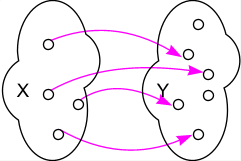
\includegraphics[scale=0.5]{injektiv.png}

\paragraph{Injektivität zeigen}
Injektiv wird meist direkt über die zweite Eigenschaft gemacht oder per Wiederspruchsbeweis (indirekter Beweis) mittels der ersten Eigenschaft bewiesen.

\paragraph{Eigenschaften}
\begin{itemize}
	\item Die Gleichung $f(x) = y$, $f$ ist injektiv und $y$ gegeben, verfügt über eine oder keine Lösung für $x$
	\item Eine \textit{stetige reelwertige} Funktion auf einem \textit{reelen Intervall} ist genau dann \underline{injektiv}, wenn sie in ihrem gesamten Definitionsbereich \textit{streng monoton} steigend oder fallend ist.
	\item Sind die beiden Funktionen $g, f$ injektiv, so ist die \underline{Komposition} $g \circ f$ ebenfalls injektiv
	\item Ist $g \circ f$ injektiv, so ist $f$ injektiv
	\item $f: M \rightarrow N$ ist injektiv, wenn es die \underline{links inverse} Funktion $g: N \rightarrow M$ gibt, so dass $g \circ f = \id_M$
\end{itemize}

\subsubsection{Surjektiv}\index{surjektiv}
Sei $f: M \rightarrow N$, $f$ ist surjektiv, wenn folgendes gilt:
\begin{align*}
\forall y \in N: \exists x \in M: f(x) = y
\end{align*}
Wenn also für jedes Element aus $N$ mindestens ein (können auch mehr sein) Element in $M$ gibt, dass auf das Element aus $N$ zeigt.

%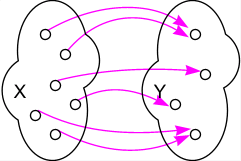
\includegraphics[scale=0.5]{surjektiv.png}

\paragraph{Eigenschaften}
\begin{itemize}
	\item Die Gleichung $f(x) = y$, $f$ ist surjektiv und $y$ gegeben, verfügt über eine oder mehrere Lösungen für $x$.
	\item Sind die Funktionen $f: A \rightarrow B$ und $g: B \rightarrow C$ surjektiv, so ist die \underline{Komposition} $g \circ f: A \rightarrow C$ auch surjektiv
	\item Ist $g \circ f$ surjektiv, so folgt, dass $g$ surjektiv ist
	\item $f: A \rightarrow B$ ist genau dann surjektiv, wenn $f$ ein \underline{rechtes Inverse} hat, also $g: B \rightarrow A$ mit $f \circ g = \id_B$
\end{itemize}

\subsubsection{Bijektiv}\index{bijektiv}
Eine Funktion ist bijektiv, wenn sie injektiv und surjektiv ist.

%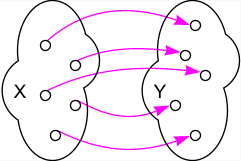
\includegraphics[scale=0.5]{bijektiv.png}
\vspace{-0.5cm}
\paragraph{Eigenschaften}
\begin{itemize}
	\item Es gelten die Eigenschaften von Injektivi. und Surjektivi.
	\item Die Gleichung $f(x) = y$, $f$ ist bijektiv und $y$ gegeben, verfügt über genau eine Lösung für $x$
	\item Sind die Funktionen $f: A \rightarrow B$ und $g: B \rightarrow C$ bijektiv, dann ist auch die \underline{Komposition} $g \circ f: A \rightarrow C$ bijektiv.
	\item Ist $g \circ f$ bijektiv, dann ist $f$ injektiv und $g$ surjektiv
\end{itemize}

\subsection{Absolutbetrag}
\begin{itemize}
	\item $|x| = \max(x, -x)$ oder 
	$\begin{array}{l}
		x \geq 0 \Rightarrow |x| = x \\
		x < 0 \Rightarrow |x| = -x
	\end{array}$
	\item $|x \cdot y| = |x| \cdot |y|$
	\item $|x + y| \leq |x| + |y|$
	\item $|x - a| < \epsilon \; \Leftrightarrow \;  -\epsilon < x- a < \epsilon \; \Leftrightarrow \; a - \epsilon < x < a + \epsilon$
	\item $|x - a| \Leftrightarrow |a - x|$
\end{itemize}

\subsection{Monotonie}
Die Funktion $f$ ist\ldots
\begin{description}
	\item[monoton steigend,] falls: $x_1 < x_2 \Rightarrow f(x_1) \leq f(x_2)$
	\item[streng monoton steigend,] falls: $x_1 < x_2 \Rightarrow f(x_1) < f(x_2)$
	\item[monoton fallend,] falls: $x_1 < x_2 \Rightarrow f(x_1) \geq f(x_2)$
	\item[streng monoton fallend,] falls: $x_1 < x_2 \Rightarrow f(x_1) > f(x_2)$
\end{description}

\subsubsection{Monotonie und Differenzial (Ableitung)}\index{monoton}
Ist $f$ auf dem Intervall $I$ differenzierbar, so gilt
\begin{itemize}
	\item $f'(x) > 0 \; \forall x \in I \Rightarrow f$ streng monoton steigend
	\item $f'(x) \geq 0 \; \forall x \in I \Leftrightarrow f$ monoton steigend
	\item $f'(x) < 0 \; \forall x \in I \Rightarrow f$ streng monoton fallend
	\item $f'(x) \leq 0 \; \forall x \in I \Leftrightarrow f$ monoton fallend
\end{itemize}

\section{Zwischenwertsatz}
Sei $f: [a,b] \to \R$ eine stetige reele Funktion, die auf einem Intervall
definiert ist. Dann existiert zu jedem $u \in [f(a), f(b)]$ (falls $f(a) \leq
f(b)$, sonst $u \in [f(b), f(a)]$) ein $c \in [a,b]$, sodass gilt: $f(c)= u$.

\subsection{Beispiel (Fixpunkt)}
Sei $f: [0,1] \to [0,1]$. Zeige: $f$ hat einen Fixpunkt, d.h. es gibt ein $x
\in [0,1]$ derart, dass $f(x) = x$.

Man erzeugt die Funktion $g: [0,1] \to \R, g(x) := f(x) - x$. Es gilt: $f(x) =
x \Leftrightarrow g(x) = 0$, d.h. ein Punkt x ist genau dann ein Fixpunkt von
$f$ wenn er eine Nullstelle von $g$ ist. Es ist zu zeigen, dass $g$ immer eine
Nullstelle auf $[0,1]$ hat. Als Differenz von zwei stetigen Funktionen ist $g$
stetig. Weil ausserdem $f(x) \in [0,1] \; \forall x \in [0,1]$ gilt, ist $g(0)
\geq 0 \geq g(1)$. Da $g$ stetig ist, gibt es daher nach dem Zwischenwertsatz
ein $x \in [0,1]$ mit $g(x) = 0$ und somit gibt es $f(x) = x$.

\section{Folgen in $\R$}
Eine Folge $a_n$ ist eine Funktion von $\N \backslash \{0\} \to \R$. Man nennt $(a_1, a_2, .. )$ Folgenglieder. Bsp. $a_n = 1/n \Rightarrow$  $a_1 = 1, a_2 = 1/2, ..$  

\subsection{Definitionen}
\begin{description}
  \item[konvergent] $\lim_{x \to \infty} a_n$ existiert \index{konvergent}
  \item[divergent] $\lim_{x \to \infty} a_n$ existiert nicht \index{divergent}
  \item[Nullfolge] $\lim_{x \to \infty} a_n = 0$ gilt \index{Nullfolge}
  \item[beschränkt] $\exists \, C_1, C_2 \in \R$, sodass gilt: $C_1 \leq a_n \leq C_2$ \hspace{0.3cm} oder\\
  $\exists \, C$ sodass gilt: $|a_n| \leq C$
  \item[unbeschränkt] falls $(a_n)$ nicht beschränkt ist. Unbeschränkte folgen
  sind stets \underline{divergent}
  \item[monoton wachsend] $a_n \leq a_{n+1} \quad \forall n \in \N$ \index{monoton}
  \item[streng monoton wachsend] $a_n < a_{n+1} \quad \forall n \in \N$
  \item[monoton fallend] $a_n \geq a_{n+1} \quad \forall n \in \N$
  \item[streng monoton fallend] $a_n > a_{n+1} \quad \forall n \in \N$
  \item[alternierend] {\small die Vorzeichen der Folgenglieder wechseln sich ab}
  \item[bestimmt divergent / uneigentlich konvergent] es gilt $\lim_{n \to
  \infty} a_n = \pm \infty$
\end{description}

\begin{definition}[Konvergenz / Grenzwert] \index{Konvergenz / Grenzwert}
Die Folge $a_n$ konvergiert gegen a falls gilt:\\
\vspace{-0.3cm}\begin{align*}
\forall \epsilon > 0 \; \exists \, n_0 \in \N \; \forall n \geq n_0: |a_n - a| < \epsilon
\end{align*}
Wir nennen $a$ den Grenzwert/Limes und schreiben dann:
\begin{align*}
	\lim_{n \to \infty} a_n = a
\end{align*}
\end{definition}

\begin{definition}[Teilfolge] \index{Teilfolge}
Werden von einer Folge beliebig viele Glieder weggelassen, aber nur so viele,
dass noch unendlich viele übrigbleiben, so erhält man eine Teilfolge.
Konvergiert eine Folge $a_n$ gegen a, so konvergiert auch jede Teilfolge gegen $a$!
\end{definition}

\begin{definition}[Häufungspunkt] \index{Häufungspunkt}
	Ein Häufungspunkt ist ein Grenzwert einer Teilfolge (Bsp. H-Punkte von $(-1)^n$ = $\{1, -1\}$). \\
	Anderst ausgedrückt: 
	$a$ ist Häufungspunkt der Folge $(a_n)$, wenn in jeder Umgebung von $a$
	unendlich viele Folgeglieder liegen.
\end{definition}

\begin{definition}[Limes superior / Limes inferior] \index{$\limsup$}\index{$\liminf$}
	Ist $a_n$ eine beschränkte Folge so heisst der grösste Häufungspunkt Limes
	superior ($\limsup_{n \to \infty} a_n$ / $\overline{\lim}_{n \to \infty}
	a_n$) und der kleinste Häufungspunkt Limes inferior ($\liminf_{n \to
	\infty} a_n$ / $\underline{\lim}_{n \to \infty} a_n$)
\end{definition}

\subsection{Cauchy-Folgen}\index{Cauchy-Folge}
\begin{definition}
Sei $(a_n)_{n \in \N}$ eine Folge in $\R$. $(a_n)_{n \in \N}$ heisst \textbf{Cauchy-Folge}, falls gilt
\begin{align*}
\forall \epsilon > 0 \; \exists \, n_0 \in \N \; \forall n, l \geq n_0: |a_n - a_l| < \epsilon
\end{align*}
\end{definition}

Die Definition sagt grundsätzlich aus, dass ab einem $n_0$ (also einem Anfang $n_0$, der nur abhängig von $\epsilon$ ist)
die Folgeglieder nur noch $\epsilon$ Abstand zu einander haben. Also der Abstand beliebig klein wird zwischen Folgegliedern.

\begin{satz}[Cauchy-Kriterium]
Für $(a_n)_{n \in \N} \subset \R$ gilt:
\begin{align*}
	(a_n) \; \text{ist konvergent} \; \Leftrightarrow \; (a_n) \; \text{ist eine Cauchy-Folge}
\end{align*}
\end{satz}


\subsection{Rechnen mit Eigenschaften}
Addition:
{\small
\begin{itemize}
  \item $(a_n), (b_n)$ konvergiert $\Rightarrow (a_n + b_n)$ konvergiert
  \item $(a_n)$ konvergiert, $(b_n)$ divergent $\Rightarrow (a_n + b_n)$
  divergent
  \item $(a_n)$ beschränkt, $(b_n)$ beschränkt $\Rightarrow (a_n + b_n)$
  beschränkt
  \item $(a_n)$ beschränkt, $(b_n)$ unbeschränkt $\Rightarrow (a_n + b_n)$
  unbeschränkt
  \item $(a_n)$ beschränkt, $(b_n) \to \pm \infty \Rightarrow (a_n + b_n) \to
  \pm \infty$
  \item $(a_n) \to \infty$, $(b_n) \to \infty \Rightarrow (a_n + b_n) \to \infty$
  \item $(a_n) \to -\infty$, $(b_n) \to -\infty \Rightarrow (a_n + b_n) \to
  -\infty$
\end{itemize}
}

Produkt:
{\small
\begin{itemize}
  \item $(a_n)$ Nullfolge, $(b_n)$ beschränkt $\Rightarrow (a_n b_n)$ Nullfolge
  \item $(a_n)$ konvergent, $(b_n)$ beschränkt $\Rightarrow (a_n b_n)$
  beschränkt
  \item $(a_n)$ konvergent, $(b_n)$ konvergent $\Rightarrow (a_n b_n)$
  konvergent
  \item $(a_n)$ konvergent gegen $a \neq 0$, $(b_n)$ divergent $\Rightarrow
  (a_n b_n)$ divergent
\end{itemize}
}

\subsection{Rechnen mit Grenzwerten}
$\lim_{n \to \infty} a_n = a$, $\lim_{n \to \infty} b_n = b$\\
\emph{\underline{Achtung!} Untenstehendes gilt \underline{nur} wenn die Grenzwerte von $a_n$ und $b_n$ existieren. (Nicht $0$ oder $\infty$ sind.)}
\begin{itemize}
  \item $\lim_{n \to \infty} (a_n \pm b_n) = a \pm b$
  \item $\lim_{n \to \infty} (c \cdot a_n) = c \cdot a$
  \item $\lim_{n \to \infty} (a_n \cdot b_n) = a \cdot b$
  \item $\lim_{n \to \infty} (a_n)^c = (\lim_{n \to \infty} a_n)^c, \quad$ nur wenn $c \neq n$
  \item $\lim_{n \to \infty} \frac{a_n}{b_n} = \frac{a}{b}, \quad$ nur wenn $(b_n)$ keine Nullfolge
\end{itemize}

\subsection{Hilfsmittel}
\textbf{Bernoullische Ungleichung}: Für $x \geq -1$ und $n \in \N$
\[
	(1+x)^n \geq 1 + nx
\]


\textbf{Vergleich von Folgen}: weiter rechts stehende Werte gehen schneller nach
$\infty$
\[
	1, \quad \ln n, \quad n^\alpha \; (\alpha > 0), \quad q^n \; (q > 1), \quad n!,
	\quad n^n
\]

\textbf{Stirlingformel}:
\[
	n! \approx \sqrt{2 \pi n} \left (\frac{n}{e} \right )^n
	\Rightarrow \left ( \frac{n}{e} \right )^n \sqrt{2 \pi n} \leq n! \leq \left (
	\frac{n}{e} \right )^n \sqrt{2 \pi n} \cdot e^\frac{12}{n}
\]

\subsection{Konvergenzkriterien}\index{Konvergenzkriterien}
\begin{align*}
	a_n \to a \Leftrightarrow a_n - a \to 0 \Leftrightarrow |a_n - a| \to 0
\end{align*}
	
\begin{itemize}[leftmargin=*]	
	\item Ist $\lim_{n \to \infty} a_n = a$, so ist der Limes $a$ einziger
	Häufungspunkt der Folge $(a_n)$ und jede Teilfolge konvergiert auch gegen $a$.
	
	\textbf{Beispiel:} Wegen $\left( 1 + \frac{1}{n} \right)^n \to e$, so gilt auch
	$\left( 1 + \frac{1}{2n} \right)^{2n} \to e$
	
	\item \textbf{Divergenzkriterium:} Hat die Folge zwei verschiedene Häufungspunkte, so ist die Folge sicher
	divergent.
	
	\item \textbf{Monotone konvergenz:} Ist die Folge monoton steigend (fallend) und nach oben (unten) beschränkt, dann konvergiert $\lim_{n \to \infty} a_n$ zu $\sup \; a_n$ $(\inf \; a_n)$
	
	\item Wenn $\sum_{n=0}^\infty a_n$ konvergiert, so ist $\lim_{n \to \infty} a_n = 0$\\
	Damit kann man die Grenzwertregeln für Reihen verwenden.
	
	\item Gibt es eine Funktion $f$ mit $f(n) = a_n$ und $\lim_{x \to \infty} f(x)
	= a$, so gilt auch $\lim_{n \to \infty} a_n = a$.\\
	Damit kann man zum Beispiel die Regel von \underline{l'Hospital} und die
	restlichen Methoden anwenden. Siehe Grenzwerte von Funktionen.
	\underline{Achtung:} Es kann sein, dass $f$ keinen Grenzwert besitzt, aber
	$(a_n)$ schon.
	
	\item \textbf{Einschliessungskriterium}: Sind $(a_n), (b_n), (c_n)$ Folgen mit
	$a_n \leq b_n \leq c_n$ und haben $(a_n), (c_n)$ den gleichen Grenzwert $a$, so
	konvergiert auch $(b_n)$ nach $a$.

	\item \textbf{Cauchy-Kriterium:} \\
	Die Folge $a_n$ ist konvergent $\Leftrightarrow$ $a_n$ ist eine Cauchy-Folge 
\end{itemize}

\subsection{Konvergenztipps \& Beispiele}
\subsubsection{Faktoren klammern und kürzen / Brüche}
Bei Brüchen und auch sonst empfiehlt es sich oft den am stärksten wachsenden Teil (das am
schnellsten wachsende $n$) zu kürzen. In diesem Fall ist es das $n^4$ in der
Wurzel, also $n^2$.
\vspace{0.1cm}
\begin{align*}
\lim_{n \to \infty} \frac{n^2 + \ln n}{\sqrt{n^4 - n^3}} 
&= \lim_{n \to \infty} \frac{n^2 + \ln n}{\sqrt{n^4 - n^3}} 
\cdot \frac{\frac{1}{n^2}}{\frac{1}{n^2}} = \lim_{n \to \infty} \frac{n^2 + \ln
n}{n^2 \sqrt{1 - \frac{1}{n}}} \cdot \frac{\frac{1}{n^2}}{\frac{1}{n^2}} \\
&= \lim_{n \to \infty} \frac{1 + \frac{\ln n}{n^2}}{\sqrt{1 - \frac{1}{n}}}
= \frac{1 + 0}{\sqrt{1 - 0}} = 1
\end{align*}

\subsubsection{l'Hospital für Folgen (Folge als Funktion)}
$\lim_{n \to \infty} \frac{\ln n}{n^2}$

Die Funktion $f(x) = \frac{\ln x}{x^2}$ entspricht unseren Folgegliedern ($f(n)
= a_n = \frac{\ln n}{n^2}$). Für $n \to \infty$ hat der Nenner und der Zähler
den Grenzwert $\infty$, also wenden wir die Regel von l'Hospital an.

\begin{align*}
\ldots &= \lim_{x \to \infty} \frac{(\ln x)'}{(x^2)'} = \lim_{x \to \infty}
\frac{\frac{1}{x}}{2x} = \lim_{x \to \infty} \frac{1}{2x^2} = 0
\end{align*}

Somit geht auch die Folge gegen 0.

\subsubsection{Wurzeln}
$\lim_{n \to \infty} (\sqrt{n^2 + an + 1} - \sqrt{n^2 + 1})$

Die einzelnen Terme streben jeweils gegen unendlich und \\
$(\infty - \infty)$ kann nicht direkt berechnet werden. Deshalb macht man hier eine Brucherweiterung \underline{mit geändertem Vorzeichen} in der Mitte!
\begin{align*}
&= \lim_{n \to \infty} (\sqrt{n^2 + an + 1} - \sqrt{n^2 + 1}) \cdot
\left(\frac{\sqrt{n^2 + an + 1} + \sqrt{n^2 + 1}}{\sqrt{n^2 + an + 1} +
\sqrt{n^2 + 1}} \right) \\
&= \lim_{n \to \infty} \frac{(n^2 + an + 1) - (n^2 + 1)}{\sqrt{n^2 + an + 1} +
\sqrt{n^2 + 1}} \\
&= \lim_{n \to \infty} \frac{an}{\sqrt{n^2 + an + 1} + \sqrt{n^2 + 1}} 
\end{align*}

nun verwenden wir den Tipp für Brüche und kürzen das $n$ heraus

\begin{align*}
\ldots &= \lim_{n \to \infty} \frac{a}{\sqrt{1 + \frac{a}{n} + \frac{1}{n^2}} +
\sqrt{1 + \frac{1}{n^2}}} = \frac{a}{1 + 1} = \frac{a}{2}
\end{align*}

\subsubsection{Einschliesskriterium}
Vereinfache $a_n$ zu $b_n$ und $c_n$ so dass gilt: $b_n \leq a_n \leq c_n$. \\
Die Grenzwerte von $b_n$ und $c_n$ sollten einfach auszurechnen sein! 
Wenn $b_n$ und $c_n$ gegen $a$ strebt, dann macht dies auch $a_n$.

\subsubsection{Laufvariable im Exponent}
$\lim_{x \to 0} (3 - |x|)^{\frac{\sin(x)}{x}}$\newline
Verwende $(x = e^{\ln x})$ Also: $(3 - |x|)^{\frac{\sin(x)}{x}} = e^{\frac{\sin(x)}{x} \cdot \ln(3 -
|x|)}$\newline
$\Rightarrow 
\lim_{x \to 0} (3 - |x|)^{\frac{\sin(x)}{x}} = \lim_{x \to 0}e^{\frac{\sin(x)}{x} \cdot \ln(3 -
|x|)}$\newline
$\Rightarrow \lim_{x \to 0}\frac{\sin(x)}{x}\cdot \ln(3-|x|) = \ln(3)$\newline
$\Rightarrow \lim_{x \to 0}(3 - |x|)^{\frac{\sin(x)}{x}} = e^{\ln(3)} = 3$


\subsubsection{Gruppieren}
%Aus Analysis II (2012) Serie 1 Aufgabe 2b
Hat man zum Beispiel die Folge $s_n = 1 + \frac{1}{3} + \frac{1}{5} + ... + \frac{1}{2n-1}$ so kann man die 
einzelnen Therme gruppieren und abschätzen in diesem Fall z.B. mit $\frac{1}{4}$ (zweiter Therm, dritter und vierter Therm,
fünfter bis achter Therm, nächste 8 Therme, etc.). Wir erhalten dann $s_{2^k} \geq 1 + \frac{k}{4}$ und sehen somit das die 
Reihe nicht beschränkt ist und somit auch nicht konvergiert.
\section{Reihen}

\subsection{Definitionen}
Eine Reihe $\sum_{n = 1}^\infty a_n$ ist \underline{konvergent} mit Grenzwert
$s$, wenn die Folge der \underline{Partialsummen} $(S_m)$, $S_m :=
\sum_{n=1}^m a_n$ gegen $s$ konvergiert. Also wenn gilt: $S_m \to s$.

\begin{definition}[$\epsilon$-Kriterium] Die Reihe konvergiert genau dann wenn gilt:
	$\; \forall \epsilon > 0 \; \exists n_0 \in \N \; \forall m \geq n_0: \left|
	\sum_{n=1}^m a_n - s \right| < \epsilon$
\end{definition}

\begin{definition}[Absolute Konvergenz]\index{Konvergenz}
Eine Reihe $\sum_{n=1}^\infty a_n$ heisst absolut konvergent falls $\sum_{n=1}^\infty |a_n| < \infty$. \\
Merke: absolute Konvergenz $\Rightarrow$ Konvergenz.
\end{definition}

\subsection{Rechenregeln Reihen}
Für \underline{absolut konvergente} Reihen gilt:
\[
	\sum_{n=1}^\infty a_n = A, \sum_{n=1}^\infty b_n = B \Rightarrow
	\sum_{n=1}^\infty (\alpha a_n + \beta b_n) = \alpha A + \beta B
\]

\subsection{Konvergenzkriterien}
\begin{tabular}{|l|}
\hline
	Konvergiert $\sum_{n=1}^\infty a_n$, so ist $\lim_{n \to \infty} a_n = 0$.\\
	Wenn also $\lim_{n \to \infty} a_n \neq 0$, so konvergiert die Reihe
	\underline{nicht}\\
\hline
\end{tabular}

\subsubsection{Reihen Kriterien}
Achtung. Die nachfolgenden Kriterien sagen nur aus, ob die Reihen konvergiert
oder nicht. Sie sagen \underline{nicht} aus, gegen was sie konvergieren!

\paragraph{Quotientenkriterium}
\[
\left| \frac{a_{n+1}}{a_n} \right| \to q. \quad \text{Dann gilt} \begin{cases}
q < 1 & \Rightarrow \sum_{n=1}^\infty a_n \text{ konvergiert absolut} \\
q = 1 & \Rightarrow \text{keine Aussage}\\
q > 1 & \Rightarrow \sum_{n=1}^\infty a_n \text{ divergiert}
\end{cases}
\]

\paragraph{Wurzelkriterium}
\[
\sqrt[n]{\left | a_n \right |} \to q. \quad \text{Dann gilt} \begin{cases}
q < 1 & \Rightarrow \sum_{n=1}^\infty a_n \text{ konvergiert absolut}\\
q = 1 & \Rightarrow \text{keine Aussage}\\
q > 1 & \Rightarrow \sum_{n=1}^\infty a_n \text{ divergiert}
\end{cases}
\]

\paragraph{Leibnizkriterium}
\vspace{-0.3cm}
{\small
Wenn nachfolgende Punkte alle gelten, dann konvergiert $\sum_{n=1}^\infty a_n$}
\begin{itemize}[leftmargin=0.5cm]
  \item $a_n$ ist alternierende Folge, dh: Vorzeichen wechselt jedes Mal
  \item $a_n \to 0$ oder $|a_n| \to 0$
  \item $|a_n|$ ist monoton fallend
\end{itemize}

\paragraph{Integralkriterium / Konvergenzkriterium}
\vspace{-0.2cm}
Sei $f$ eine monoton fallende Funktion (Folge) die nur positive Werte annimmt und auf $[a, \infty)$ mit $a \in \Z$ definiert ist, so gilt:
\[
	\sum_{n = a}^{\infty} f(n) \text{ konvergiert} \Leftrightarrow \int_a^{\infty} f(n) \, dn 
	\text{ existiert (also $< \infty$)}
\] 

\paragraph{Majorantenkriterium / Konvergenzkriterium}
\vspace{-0.2cm}
Ist $|a_n| \leq b_n$ und $\sum_{n=1}^\infty b_n$ konvergent, so konvergiert
$\sum_{n=1}^\infty a_n$ absolut.

\paragraph{Minorantenkriterium / Divergenzkriterium}
\vspace{-0.2cm}
Ist $a_n \geq b_n \geq 0$ und $\sum_{n=1}^\infty b_n$ divergent, so divergiert
$\sum_{n=1}^\infty a_n$
\pagebreak
\paragraph{Keine Nullfolge / Divergenzkriterium}
\vspace{-0.2cm}
Wenn $a_n$ keine Nullfolge ist, divergiert die Reihe! \\
Also wenn gilt: $\lim_{n \to \infty} a_n \neq 0$ oder $\lim_{n \to \infty} |a_n| \neq 0$ \\
Beachte: Aussage gilt nur in diese Richtung! Auch wenn $a_n$ eine Nullfolge ist, kann die Reihe immer noch divergieren!

\subsection{Potenzreihe}
\vspace{-0.2cm}
Die Potenzreihe hat die allgemeine Form
\[
\sum_{n=0}^\infty a_n (x - x_0)^n
\]

$x_0$ ist der Entwicklungspunkt der Potenzreihe und $(a_n)_{n \in \N}$ eine
beliebige Folge.

\subsubsection{Konvergenzradius}
\vspace{-0.2cm}
Die Berechnung des Konvergenzradius ist für Potenzreihen einfacher, da der
Faktor $(x - x_0)$ nicht analysiert werden muss. Entsprechend gilt für den
Konvergenzradius $r$ nach Wurzel- bzw. Quotientenkriterium:\\
$r = \frac{1}{\limsup_{n\to\infty} \sqrt[n]{\|a_n\|}}$ bzw.
$r = \lim_{n\to\infty} \left | \frac{a_n}{a_{n+1}} \right |$ \\
Dann gilt:
$
\begin{cases}
	|x - x_0| < r & \Rightarrow \text{ Potenzreihe konvergiert} \\
	|x - x_0| = r & \Rightarrow \text{ keine Aussage}\\
	|x - x_0| > r & \Rightarrow \text{ Potenzreihe divergiert}
\end{cases}
$

\subsection{Tips zu Konvergenz/Divergenz}
\vspace{-0.2cm}
\begin{description}
	\item [Quotientenkriterium] Gut für Reihen, die Fakultäten $n!$ oder Glieder der Form $a^n$ enthalten. Nicht auf Reihen anwendbar, in denen die Glieder nur Form $n^a$ haben.

	\item [Wurzelkriterium] Gut in Reihen, deren Glieder Form $a^n$ enthalten. Zusammen mit Stirlingformel auch auf Fakultäten anwendbar.

	\item [Leibnizkriterium] Nur für alternierende Reihen.

	\item [Integralkriterium] Anwendbar auf Reihen mit monoton fallenden Folgenglieder.

	\item [Majoranten- und Minorantenkriterium] Gut wenn Glieder einfach abgeschätzt werden können.
\end{description}

\subsection{Tips zu Konvergenz ausrechnen}
\paragraph{Brüche}
\vspace{-0.2cm}
Um zu prüfen ob die Reihe konvergiert, ist es bei Brüchen oft sinvoll das Quotientenkriterium anzuwenden. Vorallem wenn Zähler und Nenner nur aus Produkten bestehen, oft lassen sich dann diese Faktoren wieder wegkürzen!
\[
	\sum_{n=1}^\infty \frac{n!}{n^n}: = \frac{(n+1)! \cdot n^n}{(n+1)^{(n+1)} \cdot n!} 
	= \frac{(n+1) \cdot n^n}{(n+1)^{(n+1)}} = \left( \frac{n}{n+1} \right)^n = \frac{1}{e}
\]

\paragraph{Punkte einsetzen}
\vspace{-0.2cm}
Manchmal lässt sich die Reihe nicht direkt ausrechnen, dann kann es nützlich sein, ein paar Summenglieder auszurechnen um zu schauen wie sich die Reihe entwickelt. Im besten Fall lässt sich dann die Summe durch den Grenzwert ersetzen oder man muss noch den Grenzwert der neuen Folge berechnen. 
\[
	\sum_{n=2}^\infty \frac{1}{n-1} - \frac{1}{n} = \left( 1 - \frac{1}{2} + \frac{1}{2} - \frac{1}{3} + \ldots + \frac{1}{n-1} - \frac{1}{n} \right) = 1 - \frac{1}{n}
\]
\[
	\lim_{n \to \infty} 1 - \frac{1}{n} = 1
\]

\paragraph{Umformen}
\vspace{-0.2cm}
Um eine Reihe auszurechnen kann sie oft umgeformt werden (Bsp. Konstante vor Summe) auf eine Reihe von der eine geschlossene Formel bereits bekannt ist. Siehe Formeltafel!
\pagebreak
\section{Taylorreihe / -entwicklung}
Mit Hilfe der Taylorreihe können Funktionen an der Stelle x approximiert werden. Dazu muss zuerst ein $x_0$ gewählt werden, welches nahe bei x liegt und auch möglichst leicht zu berechnen ist. Dieses $x_0$ nennt man den Entwicklungspunkt. Dann können n-glieder der Taylorreihe berechnet werden.

\subsection{Definition}
\subsubsection{Taylorreihe}
Die Taylorreihe der Funktion $f$ um den Entwicklungspunkt $x_0$:\newline
$T_f (x) = \sum_{n = 0}^\infty \frac{f^{(n)}(x_0)}{n!}(x - x_0)^n$\newline

Das $n$-te Taylorpolynom:\newline
{\footnotesize
$T_n (x; x_0) = f(x_0) + f'(x_0)(x-x_0) + \frac{f''(x_0)}{2!}(x-x_0)^2 + \ldots + \frac{f^{(n)}(x_0)}{n!}(x-x_0)^n$
}

\subsubsection{Restglied}
{\small
Das Restglied entspricht dem Fehler der Approximation.\\
Das $n$-te Restglied: \\
$R_n (x; x_0) = f(x) - T_n (x; x_0)$\\

Restglied nach Lagrange kann lediglich abgeschätzt werden da $\xi$ unbekannt ist: \\
$R_n (x; x_0) = \frac{f^{(n+1)}(\xi)}{(n+1)!} (x-x_0)^{n+1}$ für ein $\xi \in (x_0, x)$ \\
$|R_n (x; x_0)| \leq \frac{|f^{(n+1)}(\xi)|}{(n+1)!} |x-x_0|^{n+1}$ für ein $\xi \in (x_0, x)$ sd $f^{(n+1)}(\xi)$ maximal wird. Dh: Wähle $\xi$ dementsprechend das dies der Fall ist!
}

{\small
\textbf{Tip:} Wenn sich $f$ als Potenzreihe darstellen lässt oder selbst eine ist, dann ist diese Potenzreihe auch die Taylor-Reihe! Das n-te Taylor Polynom kann also auch durch ausrechnen der ersten Summenglieder (bis $x^n$ erreicht wird) berechnet 
werden, was oft einfacher ist, als n Mal abzuleiten!\\
Bsp. 4.Polynom um $x_0 = 0$ von $e^{x^2}$:  $1 + x^2 + \frac{x^4}{2!}$  (da $e^x = \sum_{n = 0}^\infty \frac{x^n}{n!}$)\\
Merke: Wenn beim ausrechnen der Summenglieder höhere Polynome als Ordnung n (hier = 4) resultieren, können diese weggelassen werden, wir sind ja nur am 4. Taylor Polynom interessiert!
}

%\subsection{Rechenregeln}
%\vspace{-0.2cm}
%\subsubsection{Addition}
%\vspace{-0.2cm}
%{\small
%$f, g$ sind $m$-mal differenzierbar:
%
%$T_m (f + g)(x;x_0) = T_m f(x;x_0) + T_m g(x;x_0)$
%}
%
%\subsubsection{Multiplikation}
%\vspace{-0.2cm}
%{\small
%$f, g$ sind $m$-mal differenzierbar:
%
%$T_m (f \cdot g)(x;x_0) = T_m(T_m f(x;x_0) \cdot T_m g(x;x_0))$
%
%\underline{Achtung}: Anschaulich bedeutet es folgendes: Man
%multipliziert die beiden Taylorreihen von $f$ und $g$ miteinander ($T_m f(x;x_0) \cdot T_m g(x;x_0)$).
%Danach entfernt man alle Terme der Ordnung $> m$.
%}

%\subsubsection{Kettenregel}
%\vspace{-0.2cm}
%{\small
%$f: A \to B, g: B \to \R$ zwei $m$-mal differenzierbare Funktionen.
%Entwickelt wird um den Punkt $x_0 \in A$ mit $g(x_0) = q$ ($q$ muss man berechnen).
%Dann gilt:
%\begin{align*}
%T_m (g \circ f)(x;x_0) &= T_m (f(g))(x;x_0)\\
%&= T_m(T_m g(x;x_0) \circ T_m f(x;q))\\
%& = T_m(T_m f(T_m g(x;x_0))(x;q))
%\end{align*}
%}
%
%\vspace{-0.5cm}
%\subsubsection{Bemerkungen / Eigenschaften / Konvergenz}
%\vspace{-0.2cm}
%{\small
%\begin{itemize}
%	\item Der Konvergenzradius kann 0 sein
%	\item Falls Taylor-Reihe konvergiert, dann ist sie nicht notwendig gleich
%	der Funktion, die sie beschreibt. Gegenbeispiel:\\
%	$f(x) = 
%	\begin{cases} e^{-\frac{1}{x}} & x > 0\\
%	0 & x \leq 0\end{cases}$
%\end{itemize}
%}
\section{Stetigkeit und Limes einer Funktion}
$\lim_{x \to a} f(x) = b$ bedeutet, dass die Funktion $f$ für $x \to a$ den
Grenzwert $b$ hat. Der Funktionswert nähert sich also immer näher an $b$ heran,
wenn $x$ sich $a$ annähert (Epsilon-Delta-Kriterium).
\[
\forall \epsilon > 0 \; \exists \delta > 0: \|x -a\| < \delta \Rightarrow
\|f(x) - f(a)\| < \epsilon
\]

Funktionsfolgen verhalten sich desweiteren wie Folgen. Es gelten also die
gleichen Eigenschaften.

%nächster satz aus wikipedia http://de.wikipedia.org/wiki/Grenzwert_(Funktion):
Existiert der Grenzwert, so konvergiert die Funktion, andernfalls divergiert sie. 
Der Grenzwert existiert nicht wenn die Funktion eine Division durch 0 enhält oder 
wenn er gegen $\infty$, resp. $-\infty$ divergiert.

\subsection{(Punktweise) Stetigkeit}
\begin{definition}[(Punktweise) Stetig] \index{(Punktweise) Stetig}
Die Funktion $f$ heisst an der Stelle $a \in \Omega$ (punktweise) stetig, falls $\lim_{x \to a} f(x) = f(a)$. Dh: wenn der Grenzwert an der a existiert und er gleich dem Funktionswert an der Stelle a ist!
\end{definition}

Charakterisierungen der Stetigkeit von $f$ im Punkt $a$:
\begin{itemize}
	\item Man kann $\lim_{x \to a} f(x)$ auch als $f(\lim_{x \to a} x)$ schreiben.
	Also die Reihenfolge zwischen Bildung des Grenzwertes und der Anwendung der
	Funktion vertauschen. Beispiel: $\lim_{x \to \infty} \sin\frac{1}{x} =
	\sin(\lim_{x \to \infty} \frac{1}{x}) = \sin(0) = 0$
	\item Es gilt linker Grenzwert = Funktionswert = rechter Grenzwert: $\lim_{x
	\nearrow a} f(x) = f(a) = \lim_{x \searrow a} f(x)$
	\item Für eine beliebige (jede) Folge $(x_n)$ mit $x_n \to a$ hat $f(x_n) \to
	f(a)$ zu gelten. Dies ist praktisch um zu zeigen, dass eine Funktion an einer
	Stelle nicht stetig ist.
\end{itemize}

Eine Funktion $f$ ist stetig, wenn sie in allen Punkten stetig ist
(``punktweise Stetigkeit'').

Es gelten folgenden Eigenschaften:
\begin{itemize}
	\item Ist $f$ und $g$ stetig in einem gemeinsamen Definitionsbereich, so sind
	$f + g, f- g, f \cdot g, \frac{f}{g}, f \circ g$ ebenfalls stetig.
\end{itemize}

\subsection{Gleichmässige Stetigkeit}
Sei $f: D \to \R$, $D \subseteq \R$, dann ist $f$ genau dann stetig wenn gilt:
\[
\forall \epsilon > 0 \; \exists \delta > 0 \; \forall x,x_0 \in D: |x - x_0| < \delta
\Rightarrow |f(x) - f(x_0)| < \epsilon
\]

Der Unterschied zur punktweisen Stetigkeit liegt darin, dass $\delta$ und
$\epsilon$ nicht auch noch von $x_0$ abhängig sind. So ist $f(x) = x^2$ zwar
(punktweise) stetig, aber nicht gleichmässig stetig. Begründung: Je weiter
rechts man zwei Punkte mit einem Abstand kleiner als $\delta$ wählt, desto
grösser wird der Abstand der beiden Funktionswerte. Dieser Abstand der
Funktionswerte müsste aber kleiner als das vorgegebene $\epsilon$ bleiben.

\subsection{Lipschitz-Stetigkeit}
Eine Funktion $f: \R \to \R$ ist Lipschitz-stetig, wenn eine Konstante $L$
existiert, so dass gilt:
\[
\forall x_1,x_2 \in \R: \|f(x_1) - f(x_2)\| \leq L \cdot \|x_1 - x_2\|
\]

\subsubsection*{Beispiel}
Zeigen sie das die alternierende harmonische Reihe \[
\sum_{n=1}^\infty (-1)^{n-1} \frac{1}{n} = 1 - \frac{1}{2} +\frac{1}{3} - \frac{1}{4} + \frac{1}{5} - ...
\]
konvergiert. Man zeige, dass der Grenzwert $L$ die Ungleichung $ \frac{1}{2} < L < \frac{1}{5}$ erfüllt.\\
\\
Die Reihe konvergiert. Sei $L_N = \sum_{n=1}^N (-1)^{n-1} \frac{1}{n}$ die N-te Partialsumme. Es gilt \[
L_2 < L_4 < L_6 < ... < L_5 < L_3 < L_1
\] und daraus folgt $L_2 = \frac{1}{2} < L < \frac{1}{5} = L_3$.


\subsection{Stetigkeit, Differenzierbarkeit, Integrierbarkeit}
Sei $f$ eine Funktion, so gilt:
\begin{itemize}
	\item $f$ differenzierbar $\Rightarrow$ $f$ stetig $\Rightarrow$ $f$ integrierbar
	\item $f$ \emph{nicht} integrierbar $\Rightarrow$ $f$ \emph{nicht} stetig $\Rightarrow$ $f$\emph{nicht} diffbar
\end{itemize}

\subsection{Abhängigkeit der Stetigkeitsbegriffe}
Sei $f$ eine reelle Funktion, so gilt:

$f$ Lipschitz-stetig $\Rightarrow$ $f$ absolut stetig $\Rightarrow$ $f$
gleichmässig stetig $\Rightarrow$ $f$ (punktweise) stetig.

\subsection{Regel von de l'Hospital}
Sei $a \in \R \cup \{\infty, -\infty\}$. Es hat zu gelten:
\begin{itemize}
  \item $\lim_{x \to a} f(x) = \lim_{x \to a} g(x) = 0 \text{ oder } \pm\infty$
  \item In der Nähe von $a$ ist $g'(x) \neq 0$
\end{itemize}
Dann ist
\[
\lim_{x \to a} \frac{f(x)}{g(x)} = \lim_{x \to a}
\frac{f'(x)}{g'(x)}
\]
Diese Regel kann man mehrfach anwenden hintereinander.


\subsection{Stetig ergänzbar}
Die Funktion $f$ heisst an der Stelle $a \notin \Omega$ stetig ergänzbar, falls $\lim_{x \to a} f(x) = b$ existiert. Also genau dann wenn die Grenzwerte von allen Seiten (Bsp. links/rechts in $\R^1$) gegen den gleichen Wert streben!

\textbf{Tip:}
\begin{itemize}
  \item Um zu zeigen das eine Funktion mit mehreren Parameter in einem Punkt \emph{nicht} stetig ergänzbar ist
	hilft es häufig die Parameter gleich zu setzen. (Häufig geht dann der Limes nicht gegen den gesuchten Punkt
	 $\Rightarrow$ die Funktion ist \emph{nicht} stetig ergänzbar.)
\end{itemize}

\section{Stetigkeit von Funktionen mit mehreren Variabeln}
\begin{definition}[Grenzwert]
Eine Funktion $f(\vec{x})$ hat einen \underline{Grenzwert} $b$ an der Stelle
$\vec{a}$, wenn für \underline{jede} vektorwertige Folge $(\vec{x}_k)_{k \in \N}$,
mit $\vec{x}_k \neq \vec{a}$, $\lim_{k \to \infty}f(\vec{x}_k) = b$ erfüllt ist
\end{definition}
\begin{definition}[Stetigkeit]
Die Funktion $f(\vec{x})$ ist stetig im Punkt $\vec{a}$, wenn für
\underline{beliebige} Folgen $(\vec{x}_k)_{k \in \N}$ mit
$(\vec{x}_k) \to \vec{a}$ gilt: $\lim_{\vec{x}_k \to \vec{a}} f(\vec{x}_k) = f(\vec{a})$
für alle $k$ gilt.
\end{definition}

\subsection{Typische Fälle}
\begin{itemize}
	\item $x$-Achse entlang: $y = 0$
	\item $y$-Achse entlang: $x = 0$
	\item Winkelhalbierende: $x = y$
\end{itemize}

\subsection*{Beispiel}
\[
f(x, y) = \begin{cases}
	\frac{4xy}{x^2 + y^2} & (x,y) \neq (0,0)\\
	0 & (x,y) = (0,0)
\end{cases}
\]

Die Funktion ist als Komposition, Addidition und Multiplikation stetiger
Funktionen überall ausser in $(0,0)$ stetig (1. Zeile). Es bleibt zu untersuchen,
ob $f$ auch in $(0,0)$ stetig ist.

Längs der $x$-Achse ($y = 0$) erhalten wir:
\begin{align*}
f(x, 0) = \frac{4x \cdot 0}{x^2 + 0^2} = 0\\
\underline{\lim_{x \to 0} f(x, 0)} = \lim_{x \to 0} 0 = \underline{0}
\end{align*}

Als nächstes untersuchen wir die Winkelhalbierende ($x = y$):
\begin{align*}
f(x, x) = \frac{4x^2}{x^2 + x^2} = \frac{4x^2}{2x^2} = 2\\
\underline{\lim_{x \to 0} f(x, x)} = \lim_{x \to 0} 2 = \underline{2}
\end{align*}

Die Funktion ist somit in $(0,0)$ nicht stetig, da
$\lim_{x \to 0} f(x, 0) \neq \lim_{x \to 0} f(x, x)$ ist.
\section{Funktionsfolgen}
\subsection{Definition}
Eine Funktionsfolge $(f_n)$ \underline{konvergiert punktweise} auf dem
Definitionsbereich $I$ gegen $f$, wenn für jedes $x \in I$ gilt $f_n(x) \to f(x)$.
\[
\forall \epsilon > 0 \; \forall x \in I \; \exists n_0 \in \N: n \geq n_0
\Rightarrow |f(x) - f_n(x)| < \epsilon
\]

Die Folge \underline{konvergiert gleichmässig} auf $I$ gegen $f$, wenn
$\sup_{x\in I} |f_n(x) - f(x)| \to 0$ gilt. Das bedeutet, dass die obere
Definition für alle $x$ \underline{dasselbe} $n_0$ verwendet und nicht jeweils
verschiedene:
\[
\forall \epsilon > 0 \; \exists n_0 \in \N \; \forall x \in I: n \geq n_0
\Rightarrow |f(x) - f_n(x)| < \epsilon
\]

\underline{Wichtig}: gleichmässige Konvergenz $\Rightarrow$ punktweise
Konvergenz. Nicht aber andersrum!

\section{Differenzierbarkeit}
\subsection{Definition}
$f$ ist in $a \in I$ differenzierbar mit der Ableitung $f'(a)$, wenn
\[
\lim_{x \to a} \frac{f(x) - f(a)}{x - a} =: f'(a) = \frac{d}{dx}f(a)
\]
existiert.

Ist $f'$ stetig im Definitionsbereich, so heisst $f$ stetig differenzierbar. Man
kann also $f$ differenzieren und bekommt mit $f'$ eine stetige Funktion. Es gilt
auch $f \in C^1(I)$. $C^n(I)$ ist die Menge der $n$-mal stetig differenzierbaren
Funktionen über dem Intervall $I$.

\subsection{Mittelwertsatz (Satz von Lagrange)}
Ist $f$ auf $[a,b]$ stetig und in $]a, b[$ differenzierbar, so gibt es ein $c
\in ]a,b[$ mit\\

% 2 columns (don't insert a new linew between minipage definition, otherwise the layout will break!)
% In order to place the text on top/middle of column next to the image \vspace{0pt} must be inserted!
% Otherwise the text will appear on bottom! Go figure..
\begin{minipage}{0.25\textwidth}
	\vspace{0pt}
	\[
	\frac{f(b) - f(a)}{b-a} = f'(c)
	\]
\end{minipage}
\begin{minipage}{0.25\textwidth}
		\vspace{0pt}
	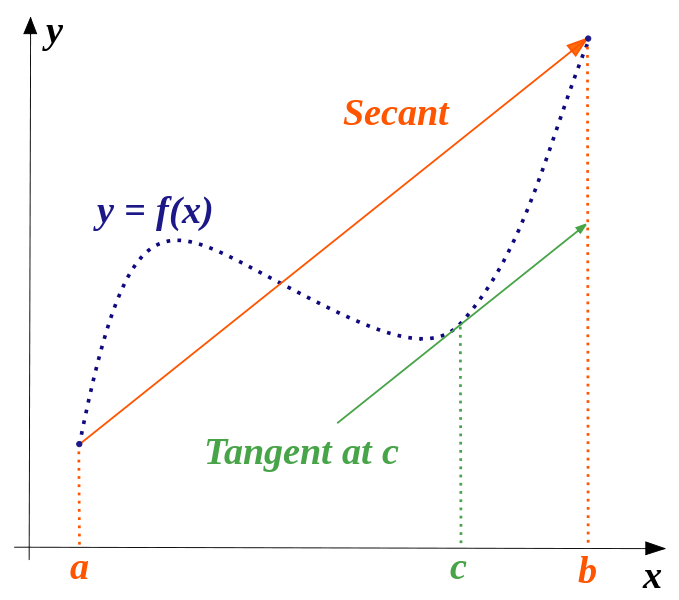
\includegraphics[scale=0.15]{mittelwertsatz.png}
\end{minipage}

\subsubsection{Beispiel: Ungleichungen}
Zu zeigen: $e^x(y-x) < e^y - e^x < e^y(y-x), \; \forall x < y$:


Der Mittelwertsatz wird auf die Exponentialfunktion angewendet. Damit gilt für
ein Paar von Zahlen $x < y$ ein $u \in ]x,y[$, für welches gilt: $\frac{e^y
- e^x}{y-x} = e^u$. Weil die Exponentialfunktion in $\R$ streng monoton wachsend
ist, gilt $e^x < e^u < e^y$ und somit gilt: $e^x < \frac{e^y-e^x}{y-x} < e^y$.
Multipliziert man nun mit dem Nenner des Bruchs bekommt man: $e^x (y-x) < e^y -
e^x < e^y(y-x)$.

\subsection{Monotonie}
\begin{itemize}
	\item $f' > 0 \Rightarrow f$ streng monoton steigend
	\item $f' \geq 0 \Leftrightarrow f$ monoton steigend
	\item $f' < 0 \Rightarrow f$ streng monoton fallend
	\item $f' \leq 0 \Leftrightarrow f$ monoton fallend
\end{itemize}
Insbesondere besitzt die Funktion $f$ wenn sie streng monoton wachsend/fallend ist
weder kritische Punkte, noch lokale oder globale Extrema.

\subsection{Konvexität}

\begin{definition}[konvex]
Eine Funktion $f: \Omega \to \R$ heisst konvex ($\cup$) , wenn $\forall x_1,x_2 \in \Omega$ und $t \in [0, 1]$ gilt:\\
$f(x_1 + t(x_2 - x_1)) \leq f(x) + t(f(x_2) - f(x_1))$
\end{definition}

\underline{Anschaulich:} Anschaulich bedeutet das, dass bei einer konvexen Funktion
der Graph immer unter der Sekante liegt. Der Graph konvexer Funktionen ist linksgekrümmt

\begin{itemize}
	\item $f'' \geq 0 \Leftrightarrow f$ konvex
\end{itemize}

\subsection{Extremstellen}
Extrema sind lokale und globale Maxima und Minima. 
\begin{itemize}
	\item Extrema bei $x_0 \Rightarrow f'(x_0) = 0$
	\item $f'(x_0) = 0, f''(x_0) > 0 \Rightarrow$ Minimum bei $x_0$
	\item $f'(x_0) = 0, f''(x_0) < 0 \Rightarrow$ Maximum bei $x_0$
	\item $f'(x_0) = 0, f''(x_0) = 0, f'''(x_0) \neq 0 \Rightarrow$ Sattelpunkt in $x_0$
	\item \hspace{1.6cm} $f''(x_0) = 0, f'''(x_0) \neq 0 \Rightarrow$ Wendepunkt in $x_0$
\end{itemize}
Merke: Jeder Sattelpunkt ist auch ein Wendepunkt!

\subsubsection{Beispiel Wendepunkt berechnen}
%Von http://www.frustfrei-lernen.de/mathematik/wendepunkt-berechnen.html
Die hinreichende Bedingung für einen Wendepunkt lautet: $f''(x_0) = 0$ und $f'''(x_0) \not= 0$\\
 
Praktische Vorgehensweise für $f(x) = \frac{1}{3}x^3-2x^2+3x$:\\
Um eine Funktion auf Wendepunkte hin zu untersuchen, führen wir die folgenden Schritte durch:
\begin{itemize}
	\item Wir leiten die Funktion f(x) dreimal ab. $f'(x) = x^2-4x+3$, $f''(x) = 2x-4$ und $f'''(x) = 2$
	\item Wir setzen die zweite Ableitung Null und berechnen den X-Wert, sofern möglich  
		$f''(x) = 2x-4 \stackrel{!}{=} 0 \Rightarrow x = 2$ 
	\item Sofern möglich, setzen wir diesen X-Wert in die dritte Ableitung ein
		$f'''(x) = 2$
	\item Ist dieses Ergebnis ungleich Null, liegt ein Wendepunkt vor
		$f'''(x) = 2 \not= 0 \Rightarrow$ Wendepunkt
	\item Der X-Wert wird in f(x) eingesetzt, um den zugehörigen Y-Wert zu bestimmen.
		$x = 2$ in $f(x)$ einsetzen: $f(2) = \frac{1}{3}2^3-2\cdot2^2+3\cdot2 = \frac{2}{3}$
\end{itemize}

\subsection{Zusammenhang zwischen Stetigkeit und Differenzierbarkeit}
\begin{itemize}
	\item differenzierbar $\Rightarrow$ stetig
	\item differenzierbar $\not\Leftarrow$ stetig
\end{itemize}

\subsection{Umkehrsatz}
% aus http://mathematik-netz.de/pdf/Umkehrsatz.pdf
Ist $f:I \to \R$ auf I differenzierbar mit $f'(x) \neq 0$ für jedes $x \in I$,
so ist $f$ streng monoton wachsend oder streng monoton fallend und damit
injektiv. Die Umkehrfunktion $f^{-1}:f(I) \to I$ existiert und ist ebenfalls
streng monoton wachsend oder streng monoton fallend. Die Ableitung
$(f^{-1})'(y)$ existiert für alle $y \in f(I)$ mit $f'(f^{-1}(y)) \neq 0)$, und zwar gilt dann \[ (f^{-1})'(y) = \frac{1}{f'(f^{-1}(y))}
\]

\subsection{Monotonie, Bijektion, Differenzierbarkeit}
\begin{satz}
(\textit{Folgendes gilt auch für streng monoton fallende Funktionen})

Sei $f: [a, b] \to \R$ stetig und streng monoton wachsend. Es sei dann
$A = f(a), B = f(b)$, dann gilt: $f: [a,b] \to [A, B]$ ist bijektiv.

$f$ hat also eine Umkehrfunktion $f^{-1}: [A,B] \to [a,b]$ und diese ist stetig
und streng monoton wachsend.
\end{satz}

\underline{Tipp:} Differentierbare Funktionen sind stetig.

\section{Partialbruchzerlegung}
Mit dieser Methode wird ein schwieriger Bruch in eine Summe von einfacheren
Brüchen zerlegt. Oft wird dies verwendet um anschliessend den Bruch einfacher integrieren zu können.

\begin{enumerate}
	\item Den Grad des Zählers und des Nenners vergleichen von $R$
	\begin{enumerate}
		\item Ist der Grad des Zählers $\geq$ der Grad des Nenners, so macht man eine 
		Polynomdivision. Man erhält daraus das Polynom $P$ und möglicherweise einen 
		Rest $R^*$, sodass gilt: $R = P + R^*$.
		\begin{enumerate}
			\item Ist $R^* \equiv 0$, so ist dieses Verfahren abgeschlossen.
			\item Sonst arbeitet man nun mit $R^*$ als Bruch weiter.
		\end{enumerate}
		\item Ist der Grad des Zählers $<$ der Grad des Nenners, so arbeitet man mit $R$ als Bruch weiter.
	\end{enumerate}
	\item Man berechnet die Nullstellen vom Nenner des Bruches (Mitternachtsformel/Raten). 
	Eine Nullstelle $x_0$ ist $r$-fach, wenn $f$ selbst und die ersten $r-1$ Ableitungen von $f$ an der Stelle $x_0$ den Wert $0$ annehmen und $f^{(r)}(x_0) \neq 0$.
	\item Nun setzt man den Bruch aus Schritt 2. gleich der Summe der
	Partialbrüche. Wie die Partialbrüche aussehen ist abhängig von den Nullstellen.  
	\begin{enumerate}
		\item Für jede einfache reelle Nullstelle $x_i$ ist der Summand
		$\frac{a_{i1}}{x-x_i}$ zu nehmen
		\item Für jede $r_i$-fache Nullstelle $x_i$ erhält man $r_i$ Summanden:
		$\frac{a_{i1}}{x-x_i} + \frac{a_{i2}}{(x-x_i)^2} + \ldots +
		\frac{a_{ir_i}}{(x-x_i)^{r_i}}$
	\end{enumerate}
	\item Nun berechnet man die unbekannten $a_{ij}$ indem man die Partialbrüche
	gleichnamig macht und dann die Koeffizienten des ursprünglichen Zählers mit
	denen des gleichnamigen Bruchs vergleicht.
\end{enumerate}

\subsection*{Beispiel}
$R(x) = \frac{x^2}{x^2-2x+1}$.

Der Zählergrad ist gleich dem Nennergrad,
weswegen wir eine Polynomdivision durchführen: $\Rightarrow R(x) = 1 +
\frac{2x-1}{(x-1)^2}$.

Aus $(x-1)^2$ folgt, das wir nur eine Nullstelle haben $x_0 = 1$. Es handelt
sich dabei um eine doppelte Nullstelle. Somit gilt:
\begin{align*}
\frac{2x-1}{(x-1)^2} &= \frac{a_1}{x-1} + \frac{a_2}{(x-1)^2}\\
2x-1 &= a_1(x-1) + a_2\\
2x-1 &= \ucomment{= 2x}{a_1 x} \;\; \ucomment{= -1 }{- a_1 + a_2}
\end{align*}
Daraus folgt, dass $a_1 = 2$ und $a_2 = 1$ (lin. Gleichungssystem).

Somit gilt: $R(x) = \frac{x^2}{x^2-2x+1} = 1 + \frac{2}{x-1} +
\frac{1}{(x-1)^2}$

\section{Integral}
\begin{theorem}[Hauptsatz der Integralrechnung] Angenommen $f:[a, b] \to \R$ ist stetig, dann definieren wir
\begin{align*}
	F(x) &= \int_a^x f(t) \, dt \\
	F'(x) &= f(x) \hspace{1cm} \forall \, x \in [a, b]\\
	\frac{d}{dx} \int_a^b f(x, t) \, dt &= \int_a^b \frac{d}{dx} f(x,t) \, dt
\end{align*}
\end{theorem}

\begin{corollary}[Stammfunktion] Jede stetige Funktion auf einem kompakten Intervall $[a,\; b]$ hat eine Stammfunktion.
\[
	\int_a^b f(x) \; dx = F(b) - F(a)
\]
\end{corollary}

\begin{corollary}[Linearität] Es gilt:
\[
	\int \alpha f(x) + \beta g(x)\,dx = \alpha \int f(x)\,dx + \beta \int g(x)\,dx
\]
\end{corollary}

\begin{definition}Falls $a < b$ ist und $f$ auf $[a, b]$ integrierbar ist, dann definieren wir:
\[
	\int_b^a f(x) \; dx = - \int_a^b f(x) \; dx
\]
\end{definition}

\vfill
\pagebreak

\subsection{Integral-Berechnung}
\subsubsection{Substitutionsregel}
Unbestimmt: $\int f(g(x)) \, g'(x) \, dx = \int f(u) \, du$ mit $u = g(x)$\\
Bestimmt: $\int_a^b f(g(x)) \, g'(x) \, dx = \int_{g(a)}^{g(b)} f(u) \, du$ mit $u = g(x)$

\begin{enumerate}
	\item Aufstellen der Substitutionsgleichungen:\\
	$u = g(x)$ und $ \frac{du}{dx} = g'(x) \Leftrightarrow du = g'(x) \, dx$ $\Leftrightarrow$ $dx = \frac{du}{g'(x)}$

	\item Durchführen der Substitution:\\
	Man ersetzt also $u = g(x)$ und $du = g'(x) \, dx$ oder $dx = \frac{du}{g'(x)}$, wobei um $dx$ zu ersetzen die erste Variante besser ist, da so auch noch $g'(x)$ aus dem Integral entfernt wird. \\
	Wenn noch $x$ übrig sind im Integral, ist ein Zwischenschritt nötig:
	Löse $u = g(x)$ nach $x$ auf, somit resultiert eine neue Formel mit 
	$x = h(u)$, substituiere nun $x$ durch $h(u)$.

	\item Berechnen des neuen Integrals nach $u$:\\
	Bei bestimmten Integralen: Sei $\int_a^b \ldots \,dx$. Dann sind die neuen
	Grenzen für das neue Integral $g(a)$ und $g(b)$

	\item Rücksubstitution:\\
	Ersetze im Ergebnis $u$ wieder mit $g(x)$. \\
	Merke: Bei einem bestimmten Integral, kann auf die Rücksubstitution verzichtet werden, wenn man die Integrationsgrenzen mitsubstituiert hat!
\end{enumerate}

\textbf{Substitutionstips:}
{\small
\begin{itemize}
	\item $\int f(ax + b) \; dx$ verwende $u = ax + b$
	\vspace{0.1cm}
	
	\item $\int f(x) \cdot f'(x) \; dx$ verwende $u = f(x)$\\
	Falls die Ableitung von $f$ ganz oder fast im Term steht!
	\vspace{0.1cm}
	
	\item $\int f(x)^n \cdot f'(x) \; dx$ verwende $u = f(x)$
	\vspace{0.1cm}

	\item $\int \frac{f'(x)}{f(x)} \; dx$ verwende $u = f(x)$\\
	Falls die Ableitung von $f$ ganz oder fast im Zähler steht!
	\vspace{0.1cm}

	\item $\int f(g(x)) \cdot g'(x) \; dx$ verwende $u = g(x)$
	\vspace{0.1cm}
	
	\item Integrale die $\sqrt{a^2 - x^2}$ enthalten: $u = a^2 - x^2$ oder\\
	$x = a \cdot \sin(u) $ und $dx = a \cdot \cos(u) \, du$ und $\sqrt{a^2 - x^2} = a \cdot \cos(u)$
	\vspace{0.1cm}

	\item Integrale die $\sqrt{a^2 + x^2}$ enthalten: $u = a^2 + x^2$ oder\\
	$x = a \cdot \sinh(u) $ und $dx = a \cdot \cosh(u) \, du$ und $\sqrt{a^2 + x^2} = a \cdot \cosh(u)$

	\vspace{0.1cm}
	\item Integrale die $\sqrt{x^2 - a^2}$ enthalten: $u = x^2 - a^2$ oder\\
	$x = a \cdot \cosh(u) $ und $dx = a \cdot \sinh(u) \, du$ und $\sqrt{x^2 - a^2} = a \cdot \sinh(u)$
\end{itemize}
\textbf{Bsp:} $\int \sqrt{1 + x^2} \; dx$\\
Wir verwenden die Substitution: $x = \sinh(u)$ mit $a = 1$. Daraus folgt aus $\frac{dx}{du}: dx = \cosh(u)$. 
Nun vollziehen wir die Substitution und erhalten: $\int \sqrt{1 + \sinh(u)^2} \cdot \cosh(u) \; du$
Aus der Formelsammlung entnehmen wir $\sqrt{a^2 + x^2} = \cosh(x)$ und ersetzen also diesen Term zu:  
$\int \cosh(u)^2 \; du$. Für diesen Typ haben wir nun in der Formelsammlung eine konkrete Lösung und es lässt sich nun leicht integrieren. Merke: Diese Ersetzungen können alle aus den Tips entnommen werden!
}

\subsubsection{Beispiel: Substitution}
$\int_0^2 x \sqrt{x+1}^3 \,dx$

Die Wurzel wird substituiert: $u = g(x) = \sqrt{x+1}$.

\begin{enumerate}[itemsep=0.5em]
	\item $\frac{du}{dx} = g'(x) = \frac{1}{2\sqrt{x+1}} = \frac{1}{2u}$. Somit
	wird $\sqrt{x+1}^3$ durch $u^3$ ersetzt und $dx$ durch
	$2u\,du$. Im Integral wären somit die Wurzel und das
	$dx$ ersetzt. Es bleibt noch das $x$ übrig vor der Wurzel. Lösen wird
	$\sqrt{x+1} = u$ nach $x$ auf, so erhalten wir $x = u^2 - 1$.
	\item Neue Grenzen: $g(0) = 1$ und $g(2) = \sqrt{3}$
	\item $\int_0^2 x \sqrt{x+1}^3 \,dx = \int_1^{\sqrt{3}} (u^2 - 1)u^3 2u \,du =
	2\int(u^6 -u^4) \,du = [\frac{2}{7}u^7 - \frac{2}{5}u^5]_{1}^{\sqrt{3}}$
	\item Rücksubstitution: $\int_0^2 x \sqrt{x+1}^3 \,dx =
	[\frac{2}{7}\sqrt{x+1}^7 - \frac{2}{5}\sqrt{x+1}^5]_{0}^{2} = \ldots = \frac{144}{35}\sqrt{3} +
	\frac{4}{35}$
\end{enumerate}

\subsubsection{Partielle Integration}
Die Formel für die Partielle Integration lautet:
\[
	\int u(x) \cdot v'(x) \, dx = u(x) \cdot v(x) - \int u'(x) \cdot v(x) \, dx
\]

In vielen Fällen lässt sich das Integral $\int f(x) \, dx$ wie folgt lösen.
\begin{enumerate}
	\item Man zerlegt $f(x)$ in geeigneter Weise in ein Produkt so dass $f(x) = u(x) \cdot v'(x)$ gilt. Man legt also einfach fest welcher Teil von $f$ dem $u$ und welcher Teil dem $v'$ entspricht (ohne dabei $f$ zu verändern!). Wähle u so, dass die Ableitung möglichst simpel ist (Bsp. $u$ = ein Polynom) damit das Integral einfacher wird.

	\item Berechne $u'$ und $v$ um es in obige Formel einzusetzen und dann das Integral zu bilden.
\end{enumerate}
Bsp: $\int \ucomment{u}{x} \, \ucomment{v'}{\cos(x)} = x \sin(x) - \int 1 \cdot \sin(x) = x \sin(x) + \cos(x) + C$\\
\textbf{Tip:} Wenn $f(x)$ aus einem Produkt mit Polynomen besteht, muss man meist das Polynom ableiten (Also u = Polynom). Eventuell mehrmals partiell integrieren. Bei jeder partiellen Integration wird so das Polynom um 1 verringert! 

\subsubsection{Allgemeine Tips}
\begin{itemize}[leftmargin=*]
	\item Hat man einen Bruch und Grad im Zähler $\geq$ Grad im Nenner. Führe immer eine Polynomdivision durch. Nun kann meist direkt ein einfacheres Resultat integriert werden. Falls immer noch zu kompliziert, siehe nächster Punkt.

	\item Hat man komplizierten Bruch und Grad im Zähler $<$ Grad im Nenner, hilft oft eine Partialbruchzerlegung.

	\item Integral mit $e^x,sin,cos$ wie: $\int_0^{\pi/2} \sin(x) \cos(2x)$ muss oft 2x partiell integriert werden und dann mit Startintegral gleichsetzen! (Wähle $v'$ so, dass Integral ohne Bruch entsteht)

	\item Integralgrenzen können aufschluss über Substitution geben.

	\item Oft besser Wurzel als Polynome auffassen, $\sqrt{x} = x^{1/2}$
\end{itemize}

% nicht relevant
%\subsubsection{Integrale mit Parametern}
%	Sei $h: \R^2 \to \R$ stetig und partiell nach $t$ diffbar mit stetiger Ableitungsfunktion. Betrachte 
%	\[ u(y) = \int_0^y h(x,y) \; \rmd x \]
%	Dann ist $u \in C^1(\R)$ und für die Ableitung gilt
%	\[ \dot{u}(y) = h(x,y)|_{x=y} + \int_0^y \frac{\partial h}{\partial y} (x,y) \; \rmd x \]

% Beispiel zu trivial
%\subsubsection{Beispiel: einfaches Integral}
%Das Integral $\int_{-2}^1 x^2 \,dx$ berechnet die blaue Fläche die durch die Funktion $f(x) = x^2$ beschränkt wird.
%$F(x)$ sei die Stammfunktion von $f(x)$,  generell berechnen wir $\int x^y \,dx = \frac{x^{(y+1)}}{y+1}$, somit $F(x) = \frac{x^3}{3}$.
%Somit $\int_{-2}^1 x^2 \,dx = F(x) \left |_{-2}^1 \right. = F(1) - F(-2) =  \frac{1^3}{3} -  \frac{-2^3}{3} = \frac{1}{3} +  \frac{8}{3} = 3.$

%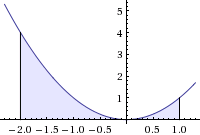
\includegraphics[scale=0.5]{integral_x2.png}

\subsection{Uneigentliche Integrale}
\begin{definition}[Uneigentliches Integral] Sei $f: \; [a, b[ \to \R$ eine Funktion. So ist das uneigentliche Integral, im Falle der Konvergenz, definiert durch (Analog für ($g: \; ]a, b] \to \R$):
\begin{align*}
	\int_a^b f(x) \; dx = \lim_{\beta \to b^-} \int_a^{\beta} f(x)\; dx\\
	\int_a^b g(x) \; dx = \lim_{\alpha \to a^+} \int_{\alpha}^{b} g(x)\; dx
\end{align*}
\end{definition}

Vorgehen:
\begin{enumerate}
	\item Kritische Stelle (Bsp. $\infty$) durch eine Variable ersetzen und Grenzwert gegen den vorherigen Wert streben lassen.

	\item Betrachte es wie ein bestimmtes Integral und berechne das Integral für die neuen Grenzen aus. 

	\item Anschliessend den Grenzwert berechnen um zu sehen, gegen welchen Wert das Resultat strebt. Wenn der Grenzwert existiert ($\neq \pm \infty$), konvergiert also das Integral und man hat das uneigentliche Integral ausgerechnet. Ansonsten divergiert der Grenzwert und somit auch das Integral
\end{enumerate}
%\vspace{-0.3cm}
{\small
\hspace{-0.35cm}
\textbf{Beispiel:}
\vspace{-0.2cm}
\begin{align*}
	\hspace{-0.35cm} \int_{a}^{\infty} f(x) \; dx = \lim_{b \to \infty} \int_a^b f(x) \; dx = \lim_{b \to \infty} \Bigl[ F(x) \Bigr]_a^b = \lim_{b \to \infty} [F(b) - F(a)] = \dots
\end{align*}}\textbf{Merke:} \\
Wenn das unbestimmte Integral innerhalb der Integralsgrenzen an einer Stelle nicht definiert oder nicht stetig ist, muss das Integral in zwei separate uneigentliche Integrale aufgeteilt werden mit dieser Stelle als Intervallsgrenze! \\

{\small
\hspace{-0.35cm}
\textbf{Beispiel:}
\vspace{-0.2cm}
\begin{align*}
	\hspace{-0.35cm} \int_{-2}^{2} \frac{1}{x} \; dx = \int_{-2}^{0} \frac{1}{x} \; dx + \int_{0}^{2} \frac{1}{x} \; dx = \lim_{b \to 0^-} \int_{-2}^{b} \frac{1}{x} \; dx + \lim_{a \to 0^+} \int_{a}^{2} \frac{1}{x} \; dx = \dots
\end{align*}}




\section{Riemannsummen (Riemannintegral)}
\subsection{Riemansumme}
Wir betrachten die folgende Einteilung des Intervals $[a,b]$:\[
E: [a,b] = \bigcup_{k=1}^{N}[x_{k-1}, x_k] \text{ mit } x_k = a + k \cdot \frac{b-a}{N}.
\]
\[
	\xi_k \in [x_{k-1}, x_k]
\]
Die Feinheit der Zerlegung ist:
\[
\Delta x = \frac{b-a}{N} \xrightarrow{N \to \infty} = 0
\]


\begin{figure}
	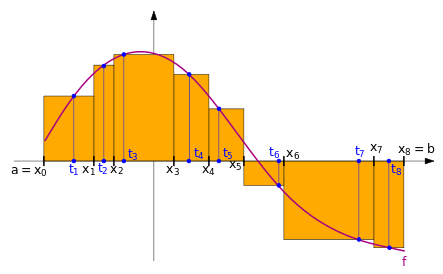
\includegraphics[width=\columnwidth]{riemann.png}
	\caption[Bildunterschrift]{Darstellung Riemannintegral mit $\xi_i = t_i$ und unsymetrischer Intervaleinteilung $E$.}
\end{figure}

Somit können wir die Riemannsumme konkret berechnen:
\begin{align*}
\int_a^b f(x)\;dx &=\sum (f,E,\xi)\\
&= \lim_{N \to \infty} \underbrace{\sum_{k=1}^{N}
	\underbrace{f(\xi_k)}_{\text{``Höhe''}} \cdot \underbrace{\Delta x}_{\text{``Länge''}}}_{\text{Riemann-Summe}}\\
&= \lim_{N \to \infty} \sum_{k=0}^{N} {f(a + k\frac{b-a}{N})} \cdot \frac{b-a}{N}
\end{align*}


\subsection{Riemann Integrierbar}
\begin{definition}[Riemann integrierbar] \index{Riemann integrierbar} Die Funktion $f$ heisst auf [a, b] Riemann integrierbar, falls der Grenzwert ($I \in \R$) existiert.
\[
	\lim_{N \to \infty} = \sum_{k = 1}^N f(\xi_k) \cdot \Delta x = I \hspace{0.5cm} \text{mit } \xi_k \in [x_{k-1}, x_k]
\]

\end{definition}

\begin{definition}[Riemann integrierbar v.2] \index{Riemann integrierbar v.2}
Die Funktion $f$ heisst auf [a, b] Riemann integrierbar falls es ein $I \in \R$ gibt sodass $\forall \epsilon > 0$ gilt:
\[
	\lim_{N \to \infty} \left| \sum_{k = 1}^N f(\xi_k) \cdot \Delta x) - I \right| < \epsilon \hspace{0.5cm} \text{mit } \xi_k \in [x_{k-1}, x_k]
\]
\end{definition}
\textbf{Merke:}\\
$f$ monoton + Definitionsbereich kompakt $\Rightarrow$ $f$ ist R integrierbar\\
$f$ stetig + Definitionsbereich kompakt $\Rightarrow$ $f$ ist R integrierbar

%\subsection*{Beispiel}
%Es soll das Intergral mittels Riemannschen Summe berechnet werden: $\int_a^b
%e^{\lambda x}\,dx, \; \lambda \in \R$. $f(x) = e^{\lambda x}$

%Zuerst unterteilt man das Intervall $[a,b]$: $E: [a,b] =
%\bigcup_{k=1}^N[c_{k-1}, c_k]$ mit $c_k = a + k\cdot \frac{b-a}{N}$.

%Die Feinheit dieser Zerlegung ist somit $\delta(E) = \max\{c_k - c_{k-1} | k =
%1 \ldots N\} = \frac{b-a}{N}$. Dabei gilt $\delta(E) = \frac{b-a}{N} \to 0$ ($N
%\to \infty$). Dies ist wichtig. Wir müssen die Feinheit unglaublich klein
%bekommen können, also nahezu $0$. Je feiner die Feinheit desto genauer wird
%unsere Riemann'sche Summe. Der Grenzwert dieser Summe für $N \to \infty$ ist der
%Wert des bestimmten Riemann-Integrals.

%Zusätzlich müssen wir festlegen, an welchen Punkten in den Teilintervallen wir
%den Funktionswert auswerten. Hier legen wir fest: $x_k = c_{k-1}$, also
%jeweils am Punkt an dem das Teilintervall beginnt.

%Daraus erhalten wir nun:
%\begin{align*}
%\int_a^b e^{\lambda x}\;dx &= \lim_{N \to \infty} \underbrace{\sum_{k=0}^{N-1}
%\underbrace{f(x_k)}_{\text{``Höhe''}} \cdot
%\underbrace{\delta(E)}_{\text{``Länge''}}}_{\text{Riemann-Summe}}\\
%&= \lim_{N \to \infty} \sum_{k=0}^{N-1} \underbrace{e^{\lambda (a +
%k\frac{b-a}{N})}}_{f(x_k)} \underbrace{\frac{b-a}{N}}_{\delta(E)}\\
%&= \lim_{N \to \infty} \frac{b-a}{N} e^{\lambda a} \sum_{k=0}^{N-1}(e^{\lambda
%\frac{b-a}{N}})^k\\
%&= \lim_{N \to \infty} \frac{b-a}{N} e^{\lambda a} \frac{1-e^{\lambda
%(b-a)}}{1-e^{\lambda \frac{b-a}{N}}}
%\end{align*}

%Wir wissen, dass $\rho = \frac{b-a}{N} \to 0$ für $N \to \infty$. Somit
%ersetzten wir es entsprechend:
%\begin{align*}
%\int_a^b e^{\lambda x}\;dx &= \lim_{\rho \to 0} \rho \cdot e^{\lambda a} \cdot
%\frac{1-e^{\lambda(b-a)}}{1-e^{\lambda \rho}}\\
%&= \lim_{\rho \to 0} \frac{\rho (e^{\lambda a} - e^{\lambda b})}{1-e^{\lambda
%\rho}}\\
%&\overset{\text{d'H}}= \lim_{\rho \to 0} \frac{e^{\lambda a} - e^{\lambda
%b}}{-\lambda e^{\lambda \rho}}\\
%&= \frac{e^{\lambda a} - e^{\lambda b}}{-\lambda} = \frac{1}{\lambda}(e^{\lambda
%a} - e^{\lambda b})
%\end{align*}
\section{Differentialgleichung (DGL)}
Lineare DGL haben die allgemeine Form:
\[
	y^{(n)} + p_{n-1}(x) \cdot y^{(n-1)} + ... + p_1(x) \cdot y' + p_0(x) \cdot y = q(x) 
\]

\begin{description}
	\item [$y$] steht für $y(x)$ eine noch unbekannte Funktion von x.\\
			$y^{(i)}$ ist einfach die $i$-te Ableitung davon.

	\item [$p_i(x)$] steht für irgendeine Funktion mit der $y$ (oder $y^{(i)}$) multipliziert wird. Kann auch eine Konstante sein (z.B. 1).

	\item [$q(x)$] nennt man Störfunktion. Ist $q(x) = 0$ nennt man die DGL Homogen, sonst Inhomogen.
\end{description}

Die allgemeine Lösung einer DGL ist gegeben durch:
\[
	y(x) = y_h(x) + y_p(x)
\]
$y_h(x)$ ist die allgemeine Lösung der Homogenen DGL und\\
$y_p(x)$ ist die partikuläre Lösung der Inhomogenen DGL.

\subsection{Lineare DGL 1. Ordnung}
Diese DGL haben die allgemeine Form: $y' + p(x) \cdot y = q(x)$

\subsubsection{Lineare DGL 1. Ordnung mit konst. Koeffizienten}
Diese DGL hat die Form: $y' + a \cdot y = q(x)$ mit $a \in \R$\\

Vorgehen: Gleich wie im Fall von n, einfach mit n = 1.

\subsubsection{Lineare DGL 1. Ordnung mit var. Koeffizienten}
Diese DGL hat die Form: $y' + p(x) \cdot y = q(x)$\\

Wir haben nur DGL mit $q(x) = 0$ behandelt.
Vorgehen: Siehe separierbare DGL.

% Nicht behandelt...
%Sei:\[
%F(x) = \int f(t) dt.
%\]
%Dann ist $\{y_{Hom}(x) = c_1e^{F(x)}| c_1 \in \R\}$ die Menge aller Lösungen der homogenen Differnentialgleichung ($y' + f(x) \cdot y = 0$). Als Ansatz für die Lösung des inhomogenen Problems setze man $y_p(x) = u(x)e^{F(x)}$, d.h. man \textit{lässt die Konstante $c_1$ variieren}. Dies ergibt eine eindeutige Zuordnung zwischen den Funktion $y$ und $u$. Denn $e^{F(x)}$ ist eine stets positive, stetig differnezierbare Funktion. Die Ableitung dieser Ansatzfunktion ist \[
%y_p'(x) = u(x)f(x)e^{F(x)} + u'(x)e^{F(x)} = y(x)f(x) + u'(x)e^{F(x)}
%\]
%Also löst $y$ die inhomogene Differntialgleichung \[
%y_p'(x) = y(x)f(x) + g(x)
%\]
%genau dann, wenn\[
%u'(x) = y(x)f(x) + g(x)
%\]
%gilt. Also folgt\[
%u(x) = \int  g(t)e^{-F(t)} dt
%\]
%Somit ist die Lösungsmenge von $y_p$
%\[
%\{ y_p'(x) = e^{F(x)} (u(x) + c_2) | c_2 \in \R \}
%\]
%Die Lösungsmenge der generellen Lösung der allgemeinen Lösung ist somit $y$:
%\begin{align*}
%&\{y\}=\{y = y_{Hom} + y_p\}\\
%& =\{ y(x) =  c_1e^{F(x)} +  e^{F(x)} (u(x) + c_2) | c_1, c_2 \in \R\} 
%\end{align*}
%Gibt es nun einen Ansatz, kann diese menge durch Einsetzen des Funktionswert und Gleichsetzen mit dem Resultat genau bestummen werde in dem die Konstanten $c$  aufgelöst werden.\\
%\\
%Konkret reicht es also aus. $F$ und $u$ zu berechnen. 

\subsubsection{Separierbare DGL}
Ist ein Spezialfall von DGL 1. Ordnung wo $q(x) = 0$ ist. Die DGL muss aber nicht zwingend linear sein! Das Ziel ist es alle $y$ und $x$ auf eine Seite zu bringen.
Eine Differentialgleichung für die Funktion $y$ heisst separierbar, wenn sie auf diese Form gebracht werden kann.
\[
	y' = p(x) \cdot h(y) \hspace{1cm} \text{Merke: $y' = \frac{dy}{dx}$}
\]
Vorgehen:
\begin{enumerate}
	\item DGL auf obige Form bringen. (wichtig: nur $y'$ links!)

	\item $y'$ mit $\frac{dy}{dx}$ ersetzen und Variabeln trennen: $\frac{1}{h(y)} \, dy = p(x) \, dx$

	\item Beidseitig integrieren: $\int \frac{1}{h(y)} \, dy = \int p(x) \, dx$

	\item Nach $y$ auflösen

	\item Lösung: $y = C \cdot e^{\int p(x) \, dx}$ \hspace{0.5cm} (Für: $h(y) = y$ und $C \in \R)$

	\item Anfangswertproblem lösen: Wenn genügend Punkte bekannt sind, kann C bestummen werden.
\end{enumerate}
\textbf{Merke:} Weitere Lösungen kann die Gleichung $h(y) = 0$ liefern, muss es aber nicht. Diese Lösungen sind konstanten (also $\in \R$).

\textbf{Beispiel:} $y' = \cos(x) \cdot y$ \\
{\small Wir bemerken, dass für $y = 0$, die DGL bereits erfüllt ist. Also ist die konstante Funktion $y_1(x) = 0$ bereits eine Lösung!}
\begin{align*}
	\frac{dy}{dx} = \cos(x) \cdot y \Leftrightarrow \frac{1}{y} \, dy &= \cos(x) \, dx\\
	\int \frac{1}{y} \, dy &= \int \cos(x) \, dx \\
	\ln(y) &= \sin(x) + C\\
	y &= e^{\sin(x) + C} \\
	y &= e^{\sin(x)} \cdot e^C \\
	 &= C' \cdot e^{\sin(x)}	\hspace{1cm} (C' \in \R)
\end{align*}


\subsubsection{genereller Ansatz}
Wenn $g(x) = 0$ ist, dann ist die DGL homogen. Falls $g(x) \neq 0$, so handelt
es sich um eine inhomogene DGL.

Der erste Schritt für homogene und inhomogene DGL ist die Lösung der homogenen
DGL: $y' + f(x) \cdot y = 0$:
{\small
\begin{align*}
y' + f(x) \cdot y &= 0 \quad \left | -(f(x) \cdot y) \right.\\
y' &= -f(x) \cdot y \quad \boxed{y' \text{ ist das gleiche wie } \frac{dy}{dx}}\\
\frac{dy}{dx} &= -f(x) \cdot y \quad \left | \div y \right.\\
\frac{dy}{dx\, y} &= -f(x) \quad \left | \int \right.\\
\int \frac{dy}{dx\, y} dx &= \int -f(x) dx \quad \boxed{\frac{dy}{dx\, y} \cdot dx = \frac{dx}{dx\, y} dy = \frac{1}{y} dy}\\
\int \frac{1}{y} dy &= \int -f(x) dx\\
\ln(y) &= -F(x) \quad \left | e^\alpha \right.\\
e^{\ln(y)} &= e^{-F(x)}\\
y &= e^{-F(x)}
\end{align*}
}

Damit erhalten wir die allgemeine Lösung: $y = A \cdot e^{-F(x)}$. Hat man eine
homogene DGL und einen Punkt, an dem die ursprüngliche Funktion ausgewertet wurde,
so kann man die explizite Lösung berechnen (also $A$ berechnen), in dem man die
hier allgemein erhaltene Lösung für den gegebenen Punkt auswertet und so die
Unbekannte bekommt.

Für ein inhomogenes DGL setzt sich die allgemeine Lösung aus der homogenen Lösung
$y_h$ und der partikulären (speziellen) Lösung $y_p$ der inhomogenen DGL zusammen.
Die homogene Lösung haben wir bereits berechnet: $y_h = A \cdot e^{-F(x)}$. Nun
folgt die partikuläre Lösung:

Dazu wird die Konstante ($A$) der homogenen Lösung als Funktion dargestellt ($u(x)$).
Wir erhalten somit: $y_p = u(x) \cdot e^{-F(x)}$.
Dieses $y_p$ setzten wir nun als $y$ in die inhomogene Gleichung ein:
{\small
\[
y' + f(x) \cdot y = g(x) \Rightarrow (\underbrace{u(x) \cdot e^{-F(x)}}_{= y_p = y})'
+ f(x) \cdot (\underbrace{u(x) \cdot e^{-F(x)}}_{= y_p = y}) = g(x)
\]
}

Die neue Gleichung wird nun nach $u'(x) = \ldots$ aufgelöst, was zu
$u'(x) = \frac{g(x)}{e^{-F(x)}}$ führt. Nun wird $u(x)$ bestimmt durch integrieren
beider Seiten: $u(x) = \int \frac{g(x)}{e^{-F(x)}}\,dx$. Hat man dies ausgerechnet,
setzt man $u(x)$ in $y_p = u(x) \cdot e^{-F(x)}$ ein und bekommt so die partikuläre
Lösung der DGL.

Als letzter Schritt für inhomogene DGL summiert man $y_h$ und $y_p$ und erhält nach
dem Umformen und Kürzen die allgemeine Lösung der DGL:
{\small
\[
y = y_h + y_p = 
\underbrace{A \cdot e^{-F(x)}}_{= y_h} +
\underbrace{\underbrace{\int \frac{g(x)}{e^{-F(x)}}\,dx}_{= u(x)} \cdot e^{-F(x)}}_{= y_p}
\]
}

Hat man für die inhomogene DGL ebenfalls Punkte an denen die Funktion ausgewertet wurde,
so kann man dies in die allgemeine Lösung eintragen und so die Unbekannten ($A$) berechnen.

\subsubsection{Beispiel mit Variation der Konstanten}
%Nach http://de.wikipedia.org/wiki/Variation_der_Konstanten#Motivation
Gegeben: $y' + x^2 \cdot y = 2x^2$\\
Somit:  $y' = f(x) \cdot y + g(x)$ mit $g(x) := 2x^2$ und $f(x) :=  - x^2$\\
Es gilt somit:\[
F(x) = \int f(t) dt. =  \int - x^2 dt. = -\frac{x^3}{3}
\]
Dann ist \[
\{y_{Hom}(x) = c_1e^{-\frac{x^3}{3}}| c_1 \in \R\}
\] die Menge aller Lösungen der homogenen Differnentialgleichung ($y' + x^2\cdot y = 0$). \\

\fbox{%
        \parbox{1\linewidth}{%
\textit{Dieser Teil muss nicht berechnet werden (Herleitung).}\\
Als Ansatz für die Lösung des inhomogenen Problems setze man $y_p(x) = u(x)e^{F(x)}$.
\\
Ansatzfunktion ist \[
y_p'(x) = u(x)f(x)e^{F(x)} + u'(x)e^{F(x)} = y(x)f(x) + u'(x)e^{F(x)}
\]
Also löst $y$ die inhomogene Differntialgleichung \[
y_p'(x) = y(x)f(x) + g(x)
\]
genau dann, wenn\[
u'(x) = y(x)f(x) + g(x)
\]
gilt.
        }%
}

Also folgt\[
u(x) = \int  g(x)e^{-F(x)} dx. =  2 \int  x^2e^{\frac{x^3}{3}} dx. = 2e^{\frac{x^3}{3}}
\]
Somit ist die Lösungsmenge von $y_p$
\[
\{ y_p'(x) = e^{-\frac{x^3}{3}} (2e^{\frac{x^3}{3}} + c_2) | c_2 \in \R \}
= \{ y_p'(x) =2 + c_3) | c_3 \in \R \}
\]
Die Lösungsmenge der generellen Lösung der allgemeinen Lösung ist somit $y$\[
\{ y(x) =  c_1e^{-\frac{x^3}{3}} +  2  | c_1 \in \R \}
\]

\subsubsection{Beispiel genereller Ansatz}
Gegeben: $y' + x^2 \cdot y = 2x^2$

Homogene DGL lösen: $y' + x^2 \cdot y = 0$
\begin{align*}
y' + x^2 \cdot y &= 0\\
\frac{dy}{dx} + x^2 \cdot y &= 0 \quad | -(x^2 \cdot y)\\
\frac{1}{dx}\, dy &= -x^2 \cdot y \quad | \div y\\
\frac{1}{dx} \frac{1}{y} \, dy &= -x^2 \quad | \int\\
\int \frac{1}{dx} \frac{1}{y} \, dy \, dx &= \int -x^2 \, dx\\
\int \frac{1}{y}\, dy &= \int -x^2 \, dx\\
\ln(y) &= -\frac{1}{3} x^3 \quad | e^\alpha\\
y &= e^{-\frac{1}{3}x^3}
\end{align*}

Somit ist die allgemeine homogene Lösung: $\underline{y_h = A \cdot e^{-\frac{1}{3}x^3}}$.


Als nächstes gehen wir die praktikuläre Lösung an:
$y_p = u(x) \cdot e^{-\frac{1}{3}x^3}$
\begin{align*}
\Rightarrow (u(x) \cdot e^{-\frac{1}{3}x^3})' + x^2 (u(x) e^{-\frac{1}{3}x^3}) &= 2 x^2\\
u'(x) \cdot e^{-\frac{1}{3}x^3} - u(x) \cdot x^2 e^{-\frac{1}{3}x^3} + u(x) x^2 e^{-\frac{1}{3}x^3} &= 2 x^2\\
u'(x) \cdot e^{-\frac{1}{3}x^3} &= 2 x^2 \quad | \div e^{-\frac{1}{3}x^3}\\
u'(x) &= 2 x^2 e^{\frac{1}{3}x^3} \quad | \int\\
u(x) &= 2 e^{\frac{1}{3}x^3}
\end{align*}

Wir erhalten somit: $\underline{y_p} = 2 e^{\frac{1}{3}x^3} \cdot e^{-\frac{1}{3}x^3} = \underline{2}$.
Die allgemeine Lösung des inhomogenen DGL ist somit:
$\underline{\underline{y}} = y_h + y_p = \underline{\underline{A \cdot e^{-\frac{1}{3}x^3} + 2}}$


\subsubsection{Beispiel Direkterer Lösungsweg}
Gegeben: $y' + x^2 \cdot y = 2x^2$.
Direkt lösen:
\begin{equation*}
\begin{array}{r l |l}
y' + x^2 \cdot y &= 2x^2\\
\frac{dy}{dx} + x^2 \cdot y &= 2x^2 \quad & -(x^2 \cdot y)\\
\frac{dy}{dx} &= 2x^2 -x^2 \cdot y \quad & \text{vereinfachen}\\
\frac{dy}{dx} &= x^2 ( 2 - y) \quad & \div (2 - y) \\
\frac{\frac{dy}{dx}}{2 - y} &= x^2  & \int \text{ with respect to } x \\
\int \frac{\frac{dy}{dx}}{2 - y}  \, dx &= \int x^2 \, dx & \text{links: } \int \frac{g'(x)}{g(x)} \, dx = \ln|g(x)|\\ 
- ln |2 - y| &= \frac{x^3}{3} + c_1 & \cdot (-1) \\
ln |2 - y| &= - \frac{x^3}{3} - c_1 & e \\
e^{ln |2 - y|} &= e^{-\frac{1}{3}x^3 - c_1 } \\
2 - y &= e^{-\frac{1}{3}x^3 - c_1 }& - 2 \\
- y &= e^{-\frac{1}{3}x^3 - c_1 } - 2 & \cdot (-1)\\
y &= - e^{-\frac{1}{3}x^3 - c_1 } + 2 & \text{replace const} \\
\underline{\underline{y}} &= \underline{\underline{c_2 \cdot e^{-\frac{1}{3}x^3} + 2}}\\
\end{array} 
\end{equation*}


\subsection{Lineare DGL n-ter Ordnung {\footnotesize mit konst. Koeffizienten}}
Diese DGL haben genau n Nullstellen und die Form:
\begin{eqnarray*}
	y^{(n)}+a_{n-1} \cdot y^{(n-1)}+\ldots+a_1 \cdot y' +a_0 \cdot y=g(x)\\
	\text{wobei} \; g(x) = 0 \hspace{10pt} \text{oder} \hspace{10pt} g(x) \neq 0
\end{eqnarray*}

\textbf{Vorgehen im homogenen Fall:}
\begin{enumerate}
	\item Homogene DGL aufstellen und dazu das charakteristische Polynom $p(\lambda)$ notieren mit Ansatz $y(x) = e^{\lambda x}$ mit $\lambda \in \C$:
	\begin{align*}
		y^{(n)} &+ a_{n-1} \cdot y^{(n-1)} &+ \ldots &+ a_1 \cdot y' &+& \, a_0 \cdot y&=0\\
		p(\lambda) = (\lambda^n &+ a_{n-1} \cdot \lambda^{n-1} &+ \ldots &+ a_1 \cdot \lambda &+& \, a_0) \cdot e^{\lambda x} &\overset{!}{=} 0 \\
		= \lambda^n &+ a_{n-1} \cdot \lambda^{n-1} &+ \ldots &+ a_1 \cdot \lambda &+& \, a_0 &\overset{!}{=} 0
	\end{align*}
	Merke: $e^{\lambda x}$ kann nie 0 sein, deshalb muss (...) = 0 sein!\\

	\item Nun müssen die ($\lambda_1, \ldots, \lambda_n$) Nullstellen von $p(\lambda)$ berechnet werden. Wenn $n > 2$ muss zuerst $p(\lambda)$ in lineare und quadratische Faktoren (durch raten/x-ausfaktorisieren/Polynomdivision/binomische Formeln) zerlegt werden. Dh: Jeder Faktor ist dann von 1. oder 2. Ordnung und davon können nun die Nullstellen berechnet werden (ablesen/Mitternachtsformel). Wir beachten, dass es sowohl reelle als auch komplexe Nullstellen gibt und merken für jede Nullstelle die Vielfachheit dieser Nullstelle.\\
	Bsp. einer linearer und quadratischen Zerlegung:
	{\small \begin{align*}
			p_1(\lambda) &= \lambda^2 + \lambda - 6 = (\lambda + 3) (\lambda - 2) \hspace{10pt} \text{oder} \\
			p_2(\lambda) &= \lambda^4 -4 = (\lambda^2 + 2) (\lambda^2 - 2) = (\lambda^2 + 2) (\lambda + \sqrt{2}) (\lambda - \sqrt{2})
	\end{align*}}
	\item 
	\begin{enumerate}[leftmargin=0.3cm]
		\item Ist $\lambda_i$ eine k-fache reelle Nullstelle, so gibt es k linear unabhängige Lösungen zur Nullstelle $\lambda_i$, nämlich:
		\vspace{3pt}
		\begin{align*}
			e^{\lambda_i x}, \, x e^{\lambda_i x}, \, x^2 e^{\lambda_i x}, \, ... , \, x^{k-1} e^{\lambda_i x}
		\end{align*}

		\item Sind $\lambda_i = a \pm ib$ k-fache komplexe Nullstellen, so gibt es 2k linear unabhängige Lösungen zu diesen 2 Nullstellen, nämlich:
		{\small\begin{align*}
				e^{\lambda_i x}, x e^{\lambda_i x}, \ldots, x^{k-1} e^{\lambda_i x}
				= \; &e^{x(a+ib)}, x e^{x(a+ib)}, \ldots, x^{k-1} e^{x(a+ib)}, \\
				&e^{x(a-ib)}, x e^{x(a-ib)} \ldots, x^{k-1} e^{x(a-ib)}
		\end{align*}}Merke: Durch anwenden der Eulersche Identität lässt sich obige komplexe Lösung auch reell schreiben als:
		\vspace{3pt}
		\begin{align*}
			&e^{a x} \, \cos(bx), \, x e^{a x} \, \cos(bx), \ldots, \, x^{k-1} e^{a x} \, \cos(bx) \hspace{10pt} \text{und}\\
			&e^{a x} \, \sin(bx), \, x e^{a x} \, \sin(bx), \ldots, \, x^{k-1} e^{a x} \, \sin(bx)
		\end{align*}
	\end{enumerate}
	\vspace{3pt}
	\item Die allgemeine Lösung dieser homogenen DGL ist nun eine linearkombination all dieser gefundenen Lösungen. \\
	Bsp: $\lambda_1 =$ einfache, $\lambda_2 = $ 2-fache reelle Nullstelle:
	\begin{align*}
	 y_h(x) = C_1 e^{\lambda_1 x} + \ucomment{\lambda_2: \text{2-fache Nullstelle}}{C_2 e^{\lambda_2 x} + C_3 x e^{\lambda_2 x}}
	\end{align*}

	\item Anfangswertproblem lösen: (nur wenn es keine inhomogene DGL ist, sonst kommt es erst später!) Vorgehen ist das gleiche wie bei inhomogenen DGL. 
\end{enumerate}

\textbf{\textbf{Vorgehen im inhomogenen Fall:}}
\begin{enumerate}
	\item Zuerst die homogene Lösung finden (siehe oben)!

	\item Dann wählt man einen geeigneten Ansatz für das $y_p$ (siehe \ref{sec:ansatz-dgl})\\
	Merke: Ist $q(x)$ eine linearkombination, dann mache die folgenden Schritte für jeden Summanden von $q(x)$ einzeln und addiere am Ende die Lösungen! (Superpositionsprinzip)

	\item Hat man einen allgmeinen Ansatz für $y_p$ mit noch unbekannten Konstanten bestummen, so werden jetzt die nächsten $n$ Ableitung davon berechnet. ($n$ = Ordnung der DGL). 

	\item Nun setzt man die berechneten Ableitungen in die ursprüngliche inhomogene DGL ein. Dh: ersetze $y$ mit $y_p$, $y'$ mit der 1. Ableitung von $y_p$ etc. Wenn möglich Terme vereinfachen.

	\item Jetzt die unbekannten Konstanten bestimmen indem man einen Koeffizientenvergleich macht. Dh: Gleichungen aufstellen, so das linke Seite der DGL der rechten entspricht. 

	\item Gefundene Konstanten können jetzt in die partikuläre Lösung eingesetzt werden.\\
	Die allgemeine Form der DGL ist $y(t) = y_h(t) + y_p(t)$

	\item Anfangswertproblem lösen: Die Unbekannten $C_i$ können gefunden werden, wenn genügend Punkte gegeben sind, an denen der Funktionswert bekannt ist. Einfach die allgemeine Lösung $y(x)$ an den gegebenen Punkten auswerten (evtl. noch ableiten) und Gleichung mit dem bekannten Resultat aufstellen.
\end{enumerate}

\subsection{Ansätze für partikuläre Lösung}
\label{sec:ansatz-dgl}
	\textbf{Hinweis}:
	\begin{itemize}
		\item Ansätze nur brauchbar für lineare DGL mit konstanten Koeffizienten.

		\item Die gesuchte Funktion $y$ ist immer vom gleichen Grad wie die Störfunktion $q(x)$.

		\item Wenn $q(x)$ eine Linearkombination von Funktionen ist, so muss man auch einen entsprechenden Ansatz wählen! Dh: Für jeden Summanden von $q(x)$ einzeln eine partikuläre Lösung finden und am Ende addieren!
	\end{itemize}
	Bezeichnungen:
	\begin{align*}
	P(x)  &  \quad \text{charakt. Polynom der DGL}  \\
	S_k(x) & \quad \text{polynomielle Störfunktion, Grad} \; k \\
	A, B & \quad \text{unbekannte Konstanten} \\
	R_k(x) = a_k x^k + . + a_1 x + a_0 & \quad \text{mit unbekannten Koeffizienten}
	\end{align*}
	
	
	
	\begin{tabular}{l|l}
		$q(x)$ & $Ansatz$ \\ \hline \hline
		
		$ S_k(x) $ & $R_k(x)$ , falls $P(0) \neq 0$\\
		\small{$S_1(x): ax + b$} &  $x^q R_k(x)$, falls $0$ $q$-fache NST von $P$ \\ 
		\small{$S_2(x): ax^2 + bx + c$} & \\ \hline

		$ c e^{mx} $  & $A e^{mx}$ , falls $P(m) \neq 0$\\ 
		&  $A x^q e^{mx}$, falls $m$ $q$-fache NST von $P$ \\ \hline

		$ S_k(x) e^{mx} $  & $R_k(x) e^{mx}$ , falls $P(m) \neq 0$\\
		&  $x^q R_k(x) e^{mx}$, falls $m$ $q$-fache NST von $P$ \\ \hline
		$ \sin wx, \cos wx $  & $A \cos wx + B \sin wx$ , falls $P(\pm iw) \neq 0$\\
		&  $x^q (A \cos wx + B \sin wx)$, falls $\pm iw$ \\
		& $q$-fache NST von $P$ \\ \hline
		$ \sinh wx, \cosh wx $  & $A \cosh wx + B \sinh wx$ , falls $P(w) \neq 0$\\
		&  $x^q (A \cosh wx + B \sinh wx)$, falls $w$ \\
		& $q$-fache NST von $P$ \\
	\end{tabular}

\section{Kurvenintegral (Linienintegral)}
In den Übungen sind nur immer Integrale der zweiten Art vorgekommen. 

\subsection{2. Art}
Das Wegintegral über ein \underline{stetiges Vektorfeld} $\vec{f}: \R^n \to \R^n$
entlang eines stetig differenzierbaren Weges $\gamma: [a,b] \to \R^n$ ist definiert
durch:
\[
\int_\gamma \vec{f}(\vec{x}) d\vec{x} := \int_a^b \left< \vec{f}(\gamma(t)), \gamma(t)' \right> dt
\]

\underline{Skalarprodukt}: $\left< \vec{a}, \vec{b} \right> = a_x b_x + a_y b_y + \ldots$

\subsubsection*{Beispiel}
%Beispiel Analysis II Serie 11 4a)
Berechne des Linienintegral $\int_\gamma \vec{K} d\vec{x} $ für $ \vec{K}(x,y) = (x^2+y, 2xy)$ und $\gamma$ als Einheitskreis mit positivem Umlaufsinn.
Gegeben:
\begin{align*}
\vec{K}(x,y) &= (x^2+y, 2xy) \\
\gamma &: [0,2\pi]  \to \R^2\\
\gamma &: t \mapsto   (\cos(t), \sin(t)) 
\end{align*}
Zu berechnen:
\begin{eqnarray*}
\gamma(t)' &=& (-\sin(t),\cos(t))\\
\vec{K}(\gamma(t)) &=& (\cos^2(t) + \sin(t), 2 \cos(t)\sin(t))\\
\left< \vec{K}(\gamma(t)), \gamma(t)' \right> &=& -\cos^2(t)\sin(t) - \sin^2(t)
+ 2\cos^2(t)\sin(t)\\
 &=& \cos^2(t)\sin(t) - \sin^2(t)
\end{eqnarray*}
\begin{eqnarray*}
\int_\gamma \vec{K} d\vec{x} &=& \int_0^{2\pi} \left< \vec{K}(\gamma(t)), \gamma(t)' \right> dt\\
&=& \int_0^{2\pi} \cos^2(t)\sin(t) - \sin^2(t) dt\\
&=& \left. -\frac{1}{3}\cos^3(t) - \frac{1}{2}t + \sin(t)\cos(t)
\right|_0^{2\pi} = \underline{\underline{-\pi}}
\end{eqnarray*}


\subsection{1. Art}
Das Wegintegral einer \underline{stetigen Funktion} $f: \R^n \to \R$ entlang
eines stetig differenzierbaren Weges $\gamma: [a,b] \to \R^n$ ist definiert durch:
\[
\int_\gamma f ds := \int_a^b f(\gamma(t)) \|\gamma(t)'\|_2 dt
\]

\underline{Euklidische Norm}: $\|\vec{a}\|_2 = \sqrt{a_x^2 + a_y^2 + \ldots}$.
Achtung: Beim Integral muss man zuerst $\gamma(t)$ nach $t$ ableiten und erst
dann die Norm davon berechnen!

\subsubsection*{Beispiel}
% Beispiel von http://www.tu-ilmenau.de/fileadmin/media/num/neundorf/Dokumente/Lehre/hm/Kurven_Integral.pdf Seite 2
Es sei die Schraubenlinie (Spirale in 3D)
\[
\gamma : [0,2\pi]  \to \R^3, \gamma : t \mapsto  (\cos(t), \sin(t), t) 
\]
und $f(x,y,z) := x^2 + y^2 + z^2$ gegeben. Wir berechnen $\int_\gamma f ds$. Zunächst bestimmen wir
\begin{align*}
\|\gamma(t)'\|_2 &= \sqrt{\left[\frac{d(\cos t)}{dt}\right]^2 +
\left[\frac{d(\sin t)}{dt}\right]^2 + \left[\frac{dt}{dt}\right]^2} \\
&= \sqrt{\sin^2(t)+\cos^2(t)+1}=\sqrt{2}
\end{align*}
Dann substituieren wir x,y und z und erhalten
\[
f(x,y,z) = f(\gamma(t)) = \sin^2(t)+\cos^2(t)+t^2 = 1 +t^2
\]
auf $\gamma$. Das führt zu
\begin{align*}
\int_\gamma f(x,y,z) ds &= \int_0^{2\pi} (1 +t^2)\sqrt{2} dt = \left. \sqrt{2}(t+\frac{t^3}{3}) \right|_0^{2\pi} \\
&= \frac{2\sqrt{2}\pi}{3}(3+4\pi^2)
\end{align*}


\subsection{Parametrisierung von Kurven}
Grundlegender Tipp: Skizze machen, um Grenzen und Kurve besser zu verstehen und
schneller auf die Parametrisierung zu kommen.

\begin{itemize}[leftmargin=*]
	\item Wenn die Kurve in der Form
	\[
	C = \{\vec{r} \in \R^n | \vec{r} = \gamma(t), a \leq t \leq b\}
	\]
	bereits gegeben, so ist klar, dass $\gamma(t)$ der Weg ist und das Integral von
	$a$ nach $b$ verläuft.
	
	\item Die Paramtrisierung einer \underline{Strecke} von $\vec{a}$ nach $\vec{b}$:
	$\gamma(t) = \vec{a} + t(\vec{b}-\vec{a}), \quad 0 \leq t \leq 1$
	
	\item Die Parametrisierung eines \underline{Kreises} mit Mittelpunkt $(x_0, y_0)$ und
	Radius $r$ ist: $\gamma(t) =
	\begin{pmatrix}
	x_0 + r \cos(t)\\
	y_0 + r \sin(t)
	\end{pmatrix}$. Für einen vollen Kreis gilt $0 \leq t \leq 2\pi$, für Kreisteile
	schränkt man diesen Intervall entsprechend ein.
	
	\item Parametrisierung eines \underline{Graphen} der Funktion $f(x)$ für $x$
	zwischen $a$ und $b$: $\gamma(t) =
	\begin{pmatrix}
	t\\
	f(t)
	\end{pmatrix}, \quad a \leq t \leq b$. \underline{Achtung:} Hat man zwei
	Graphen, die als Grenzen für das Kurvenintegral fungieren, so schliessen diese
	gemeinsam eine Fläche ein. Die Umlaufrichtung ist so zu wählen, dass diese
	Fläche jeweils links liegt.
\end{itemize}

\subsubsection{Beispiel: Kurvenintegral mit zwei Grenzgraphen}
% Analysis 2, Serie 12, Aufgabe 2b
Es soll das Kurvenintegral $\int_\gamma K(x,y)\;dt = \int_\gamma
\begin{pmatrix}
x^2 - y^2\\
2y -x
\end{pmatrix}\;dt$ berechnet werden. $\gamma$ ist der Rand des beschränkten
Gebietes im ersten Quadranten, welches durch die Graphen $y=x^2$ und $y=x^3$ begrenzt
wird.

Lösung: Man macht eine Skizze der Grenzen ($y=x^2$ und $y=x^3$) und sieht, dass
diese eine Fläche einschliessen. Die Schnittpunkte sind $x = 0$ und $x = 1$. Der
Rand dieses Gebiets besteht also aus den beiden parametrisierten Kurven
(Parametrisierung für Graphen verwenden)
\begin{align*}
\gamma_1(t) &= \begin{pmatrix}t\\t^3\end{pmatrix} & t \in [0,1]\\
\gamma_2(t) &= \begin{pmatrix}t\\t^2\end{pmatrix} & t \in [0,1]
\end{align*}

Wir sehen, dass die eingeschlossene Fläche in Durchlaufrichtung von $\gamma_1$
links liegt, was soweit gut ist. Bei $\gamma_2$ liegt die Fläche aber auf der
rechten Seite, weshalb wir die Durchlaufrichtung drehen müssen, was zu $\gamma
= \gamma_1 - \gamma_2$ führt (man beachte das Minus statt einem Plus).

Jetzt muss nur noch ganz normal das Wegintegral berechnet werden: $\int_\gamma
K\;dx = \int_{\gamma_1} K\;dx + \int_{-\gamma_2} K\;dx = \int_{\gamma_1} K\;dx -
\int_{\gamma_2} K\;dx = \ldots$

\subsection{Berechnung}
Die Berechnung findet in drei Schritten statt:
\begin{enumerate}[leftmargin=*]
	\item Parametrisierung der Kurve $C$ als $C = \{\vec{r} \in \R^n | \vec{r} = \gamma(t), a \leq t \leq b\}$
	\item Einsetzen ins Integral: $\int_C f(\vec{r})\,ds = \int_a^b f(\gamma(t)) \|\gamma(t)'\|\,dt$.
	Man setzt also für die Variabeln von $f$ die Komponenten von $\gamma$ ein und
	multipliziert dies dann mit dem Betrag der Ableitung nach $t$ von $\gamma$.
	\item Integral ausrechnen.
\end{enumerate}

\subsection{Bogenlänge}
Für die Bogenlänge L, auf dem Weg beschrieben durch $x(t)$ und $y(t)$, ergibt sich: \[
L = \int ds = \int_a^b \sqrt{\dot{x}^2 + \dot{y}^2} dt
\]


\section{Differentialrechnung in $\R^n$}
Hier geht es um Funktionen $f: \R^n \to \R^m$, wobei $m=1$ gelten kann
($f: \R^n \to \R$). Solche Funktionen haben die allgemeine Form:
$f(x) = f(x_1, x_2, x_3, \ldots, x_n) = \begin{pmatrix}
f_1(x_1, x_2, x_3, \ldots, x_n)\\
f_2(x_1, x_2, x_3, \ldots, x_n)\\
\ldots\\
f_m(x_1, x_2, x_3, \ldots, x_n)
\end{pmatrix}$

Für nahezu alle Eigenschaften gilt: Die Vektorfunktion $f: \R^n \to \R^m$ hat
eine bestimmte Eigenschaft, wenn jede einzelne ihrer Komponenten
($f_1, f_2, \ldots, f_m$) die besagte Eigenschaft besitzen. Das Problem liegt
neu also nicht im Wertebereich, sondern vor allem in Definitionsbereich.

\subsection{Norm}
Eine Norm auf $\R^n$ ist die Funktion $\|\cdot\|: \R^n \to \R$ mit den folgenden
Eigenschaften:
\begin{itemize}
	\item $\forall x \in \R^n: \|x\| \geq 0$
	\item $\forall x \in \R^n: \|x\| = 0 \Leftrightarrow x = \vec{0}$
	\item $\forall x \in \R^n, \alpha \in \R: \|\alpha x\| = |\alpha| \|x\|$
	\item $\forall x,y \in \R^n: \|x + y\| \leq \|x\|+\|y\|$
\end{itemize}

\subsection{Partielle Ableitung}
$\frac{\partial f}{\partial x} = f_{x} = $ partielle Ableitung von $f$ nach $x$. Dabei leitet man die Funktion nach $x$ ab und betrachtet die anderen Variabeln als Konstant. \\
Merke: partielle differenzierbarkeit impliziert nicht stetigkeit!

\begin{definition}A heisst die Ableitung von f (einfach jede Komponente nach jeder Variabel ableiten) und wir schreiben:
\[	
	A = Df(x)
\]
 \\
Bsp. Sei $f: \R^2 \to \R^3$ eine Funktion:\\
$f(x, y) = 
\left(
	\begin{array}{c}
		g_1(x, y) \\
		g_2(x, y) \\
		g_3(x, y)
	\end{array}
\right)$  
Dann ist: $Df(x, y) = 
\left(
	\begin{tabular}{c|c}
		\vspace{0.1cm}$\frac{\partial g_1}{\partial x}$ & $\frac{\partial g_1}{\partial y}$ \\
		\vspace{0.1cm}$\frac{\partial g_2}{\partial x}$ & $\frac{\partial g_2}{\partial y}$ \\
		$\frac{\partial g_3}{\partial x}$ & $\frac{\partial g_3}{\partial y}$
	\end{tabular}
\right)$
\end{definition}

\begin{satz}[Satz von Schwarz]
Ist $f$ nach $x$ und $y$ zweimal partiell differenzierbar und sind die gemischten
partiellen Ableitungen $f_{xy}$ und $f_{yx}$ stetig, so gilt: $f_{xy} = f_{yx}$.
\end{satz}
\section{Vektoranalysis}
\begin{definition}[Vektorfeld]
Die Abbildung $F: \R^n \to \R^n$ ist ein Vektorfeld. Es weist jedem
Vektor $\vec{x} \in \R^n$ einen Vektor $F(\vec{x}) \in \R^n$ zu.
\end{definition}

\begin{definition}[Skalarfeld]
Ist eine Abbildung der Form $f: \R^n \to \R$. Es existiert wenn das Vektorfeld wirbelfrei/konservativ ist. Ergibt ein geschlossener Weg im Vektorfeld nicht null so existiert kein skalares Feld (jedoch nicht umbedingt umgekehrt).\\
Ebenes Skalarfeld: $f: \R^2 \to \R$ (Pro Flächenpunkt ein Skalar)\\
Räumliches Skalarfeld: $f: \R^3 \to \R$ (Pro Raumpunkt ein Skalar)
\end{definition}

\begin{definition}[Gradient]
Ist $f: \R^n \to \R$ (ein Skalarfeld), so ist der Gradient von $f$ der Vektor
$\vec{v} = \grad f = \nabla f$. 

\[
	\text{Im Fall } f: \R^3 \to \R:   \nabla f = (f_x, f_y, f_z) =
	\left( \frac{\partial f}{\partial x}, \frac{\partial f}{\partial y}, \frac{\partial f}{\partial z} \right)
\]

Der Gradient ist also einfach ein Vektor, der aus den partiellen Ableitungen dieser Funktion besteht. Der Gradient beschreibt (von einem Punkt aus) immer die Richtung und den Betrag des steilsten Anstiegs der Funktion. 

Analog wird die maximale Fallrichtung bezeichnet: $- \nabla f$
\end{definition}

\begin{definition}[Richtungsvektor] Der Richtungsvektor ist ein normiert Vektor auf länge 1. Dh: Wenn die Richtung der grössten Steigung gefragt ist, ist der normierte Gradient gemeint! Also $\frac{\nabla f}{|\nabla f|}$
\end{definition}

\begin{definition}[Richtungsableitung]
Ist eine reelle Zahl, sie gibt die Änderung des Funktionswertes von $f$ an, wenn man von einem Punkt $P$ aus in eine bestimmte Richtung $\vec{a}$ um eine Längeneinheit fortschreitet. Die Richtungsableitung von $f$ in Richtung $\vec{a}$ ist definiert als: 
$\frac{\partial f}{\partial \vec{a}} = \nabla f \cdot \vec{e_a} = \nabla f \cdot \frac{\vec{a}}{|\vec{a}|} = \frac{1}{|\vec{a}|} \cdot \nabla f \cdot \vec{a}$\\
Merke: Die Richtungsableitung ist maximal, wenn $\vec{a}$ in gleiche Richtung wie Gradient zeigt!
\end{definition}

\begin{definition}[Gradientenfeld / Potentialfeld] Sei\\ 
$f: \R^n \to \R$ (ein Skalarfeld), dann ist $\vec{v} = \nabla f$ ein Vektorfeld und nennt $\vec{v}$
Gradientenfeld / Potentialfeld.\\
Es besitzt folgende Eigenschaften:
\begin{itemize}[leftmargin=0.5cm]
	\item Der Wert des Kurvenintegrals entlang eines beliebigen Weges innerhalb des
	Feldes ist unabhängig vom Weg selbst, sondern nur vom Anfangs- und Endpunkt
	\item Ein Kurvenintegral mit einem Weg bei dem Anfangs- und Endpunkt der
	gleiche Punkt sind, hat den Wert 0.
	\item Ist immer wirbelfrei: $\rot \vec{v} = \rot(\grad f) = \vec{0}$
\end{itemize}
\end{definition}

\begin{definition}[Potential]
Ist $\vec{v} = \nabla f$ (ein Potentialfeld), so ist $f: \R^n \to \R$ das Potential oder Stammfunktion zu $\vec{v}$. Gesucht ist also die Funktion $f$, welche abgeleitet das Potentialfeld $\vec{v}$ ergibt!
Existiert wenn $\rot \vec{f} = \vec{0}$ und der Definitionsbereich zusamenhängend ist.
\end{definition}

\begin{definition}[Rotor / Rotation]
Gibt die Tendenz eines Vektorfeldes an, um Punkte zu rotieren. Es ist ein Vektorfeld, welches aus einem anderen Vektorfeld hergeleitet wird. Die Rotation des Vektorfelds $F$ ist das Vektorfeld $\operatorname{rot} F$. Also: 
$F (x, y) = 
\left(
	\begin{array}{c}
		F_1 (x, y) \\
		F_2 (x, y)
	\end{array}
\right) \Rightarrow
 \operatorname{rot} F = 
\left(
	\begin{array}{c}
		\vspace{3pt} F_{2_x} - F_{1_y}
	\end{array}
\right)$\\
$F(x, y, z) = 
\left(
	\begin{array}{c}
		F_1 (x, y, z) \\
		F_2 (x, y, z) \\
		F_3 (x, y, z)
	\end{array}
\right) \Rightarrow
 \operatorname{rot} F = 
\left(
	\begin{array}{c}
		\vspace{3pt} F_{3_y} - F_{2_z} \\
		\vspace{3pt} F_{1_z} - F_{3_x} \\
					 F_{2_x} - F_{1_y}
	\end{array}
\right)$\\
Das Vektorfeld $\operatorname{rot} F$ wird häufig auch als Wirbelfeld zu $F$ bezeichnet. $F$ heisst in einem Bereich Wirbelfrei / Konservativ, wenn dort überall $\operatorname{rot} F = 0$ gilt.
\end{definition}

\begin{definition}[Wirbelfrei / konservativ]
Ein Vektorfeld $\vec{v}$ ist wirbelfrei/konservativ wenn gilt: $\rot \vec{v} = 0$
\end{definition}

\begin{definition}[Vektorpotential]
Ein Vektorfeld $\vec{v}$ heisst Vektorpotential zu $\vec{w}$, falls $\vec{w} = \rot \vec{v}$.
\end{definition}

\begin{definition}[Divergenz]
Ist eine reelle Zahl, und ist ein Mass für die ''Quellen-/Senken-stärke'' eines bestimmten Punktes. 
Die Divergenz eines Vektorfelds $F(x, y, z)$ ist definiert als div $F$. Also:
\[
F(x, y, z) = 
\left(
	\begin{array}{c}
		F_1 (x, y, z) \\
		F_2 (x, y, z) \\
		F_3 (x, y, z)
	\end{array}
\right) \Rightarrow
	\operatorname{div} F = \frac{\partial F_1}{\partial x} + \frac{\partial F_2}{\partial y} + 
	\frac{\partial F_3}{\partial z}
\] 
$
\operatorname{div} F(x_0, y_0, z_0) > 0 \Rightarrow \text{Quelle}\\
\operatorname{div} F(x_0, y_0, z_0) < 0 \Rightarrow \text{Senke}\\
\operatorname{div} F(x_0, y_0, z_0) = 0 \Rightarrow \text{Quellenfrei}
$
\end{definition}

\begin{lemma}[Geschlossener Weg]
Wenn das Vektorfeld $F$ ein Potential besitzt \uline{und} $\gamma$ geschlossen ist, so folgt $\int_\gamma F = 0$.\\
Merke: $F$ besitzt genau dann ein Potential wenn:\\
$F = \grad \phi$ oder ($\rot F = \vec{0}$ und der DB zusammenhängend ist)
\end{lemma}

\pagebreak
\subsection{Bestimmen eines Potentials im $\R^2$}
Sei $\vec{v} = \begin{pmatrix}
F_1(x,y)\\
F_2(x,y)
\end{pmatrix} \hspace{1.5cm} \text{Merke: } F_{1_x}$ steht führ: $\frac{\partial F_1}{\partial x}$.

Um schnell zu prüfen, ob man überhaupt den folgenden Algorithmus anwenden muss,
kann man prüfen ob gilt: $F_{2_x} = F_{1_y}$ (rot $\vec{v} = 0)$, wenn nicht, so hat $\vec{v}$ kein Potential $f$.

\begin{enumerate}[itemsep=1em]
	\item $f(x,y) = \int F_1(x,y)\;dx + C(y)$ berechnen (Integral berechnen)
	\item Die berechnete Gleichung $f(x,y)$ nun nach $y$ ableiten:
	$\frac{\partial}{\partial y} f(x,y) = \frac{\partial}{\partial y}\int F_1(x,y)\;dx + C'(y)$
	(berechnetes Integral nach $y$ ableiten)
	\item $\frac{\partial}{\partial y} f(x,y) = F_2(x,y)$ setzen und $C'(y)$ berechnen durch umformen
	und integrieren
	\item Berechnetes $C(y)$ in die Gleichung im 1. Punkt einsetzen. Fertig. Achtung: Im Grunde hat
	$C(y)$ durch integrieren (aufleiten) noch einen konstanten Wert, der beliebigen Wert haben kann.
	Dieser taucht im Grunde auch in der fertigen $f(x,y)$ Funktion auf.
\end{enumerate}

\subsection{Bestimmen eines Potentials im $\R^3$}
Sei $\vec{v} = \begin{pmatrix}
F_1(x,y,z)\\
F_2(x,y,z)\\
F_3(x,y,z)
\end{pmatrix}$.

Um zu prüfen, ob man überhaupt ein Potential finden kann für $\vec{v}$ hat $\rot \vec{v} = 0$
zu sein, also wirbelfrei zu sein. Dazu muss gelten (zu zeigen mit $\rot \vec{v} = 0$): 
$F_{3_y} = F_{2_z}, F_{1_z} = F_{3_x}, F_{2_x} = F_{1_y}$.

\begin{enumerate}[itemsep=1em]
	\item $f(x,y,z) = \int F_1(x,y,z)\;dx + C(y,z)$ lösen (Integral berechnen)
	\item Nun die berechnete Gleichung $f(x,y,z)$ nach $y$ ableiten $\Rightarrow f_y(x,y,z)$.
	\item Die abgeleitete Gleichung $f_y$ mit $F_2(x,y,z)$ gleichsetzen: $f_y(x,y,z) = F_2(x,y,z)$
	und damit $C_y(y,z)$ bestimmen.
	\item Durch Integration von $C_y(y,z)$ nach $y$ ($\int C_y(y,z)\;dy$) wird $C(y,z)$ bestimmt
	bis auf eine Konstante $D(z)$, die von $z$ abhängt. $C(y,z)$ hat also die Form:
	$C(y,z) = \int C_y(y,z)\; dy + D(z)$.
	\item Dieses $C(y,z)$ setzt man nun in die Gleichung $f(x,y,z)$ ein, die im 1. Punkt steht.
	\item Nun wird die daraus erzeugte
	$f(x,y,z) = \int F_1(x,y,z)\;dx + C(y,z) = \int F_1(x,y,z)\;dx + \int C_y(y,z)\; dy + D(z)$
	Gleichung nach $z$ abgeleitet.
	\item Durch Gleichsetzen von $f_z(x,y,z) = F_3(x,y,z)$ lässt sich $D_z(z)$ bestimmen.
	\item $D_z(z)$ wird wiederrum durch Integration zu $D(z) = \int D_z(z)\; dz + c, \quad c \in \R$
	\item Das berechnete $D(z)$ in die $f(x,y,z)$ Gleichung aus Punkt 6 einsetzen, fertig.
\end{enumerate}

% Kein Platz
%\subsection{Geometrisches Verständniss}
%Sei B ein drei dimensionaler Körper (beschrieben durch Punkte in $\R^3$ mit der Funktion $f$) so sei $\nabla f$ senkrecht dazu.

%\subsubsection*{Beispiel}
%aus analysis 2 (2012) serie 11 mc 3
%Gib einen Vektoren der ein nach aussen gerichteter Normalenvektor
%(nicht notwendigerweise normiert) auf dem Rand des Ellipsoids ist \[
%B := 
%\left\{ 
%	\begin{pmatrix} x\\ y\\ z \end{pmatrix} \in \R^3  
%	\middle\vert
%	f\begin{pmatrix} x\\ y\\ z \end{pmatrix} 
%		= \frac{x^2}{a^2} + \frac{y^2}{b^2} + \frac{z^2}{c^2} \leq 1
%\right\}
%\]

%Der Vektor $\begin{pmatrix} 2x/a^2\\ 2y/b^2\\ 2z/c^2 \end{pmatrix}$ ist gleich $\nabla f$ und steht somit 
%senkrecht auf der Niveaufläche $f=1$. Da er vom Ursprung weg orientiert ist, liefert er die richtige Antwort.\\
%Der Vektor $\begin{pmatrix} yz(1/b^2-1/c^2)\\ xz(1/c^2-1/a^2)\\ xy(1/a^2-1/b^2) \end{pmatrix}$ ist tangential 
%zum Rand $\partial B$

\subsection{Hesse Matrix}
Die Hesse-Matrix besteht aus den Ergebnissen, wenn $f$ zweimal hintereinander nach $x_i$ und $x_j$ partiell abgeleitet wird. Ist die Funktion zweimal stetig differenzierbar kann die Hesse-Matrix gebildet werden, welche immer symemtrisch ist (dh: $f_{xy} = f_{yx}$). \\
Also gilt für $f: \R^n \to \R$ und $i,j = 1, \ldots, n$:
\[
	H_{f(x_1, \ldots, x_n)} = 
	\left(
		\begin{array}{c}
			\frac{\partial^2 f}{\partial x_i \, \partial x_j}
		\end{array}
	\right)
\]
Für $f: \R^2 \to \R$ gilt also:
\[
	H_{f(x, y)} = 
	\left(
		\begin{array}{cc}
			f_{xx} & f_{xy}\\
			f_{yx} & f_{yy}
		\end{array}
	\right)	=
	\left(
		\begin{array}{cc}
			\vspace{0.1cm} \frac{\partial^2 f}{\partial x \, \partial x} & \frac{\partial^2 f}{\partial x \, \partial y} \\
			\frac{\partial^2 f}{\partial y \, \partial x} & \frac{\partial^2 f}{\partial y \, \partial y}
		\end{array}
	\right)
\]

\subsection{Determinante}
{\small
$
	\text{det} A = 
	\left|
		\begin{array}{cc}
			a_{11} & a_{12}\\
			a_{21} & a_{22}\\
		\end{array}
	\right| = a_{11} \, a_{22} - a_{12} \, a_{21}
$
\[
	\text{det} A = 
	\left|
		\begin{array}{ccc}
			a_{11} & a_{12} & a_{13}\\
			a_{21} & a_{22} & a_{23}\\
			a_{31} & a_{32} & a_{33}
		\end{array}
	\right| = 
	\begin{array}{c}
			a_{11} \, a_{22} \, a_{33} + a_{12} \, a_{23} \, a_{31} + a_{13} \, a_{21} \, a_{32}\\
			- a_{31} \, a_{22} \, a_{13} - a_{32} \, a_{23} \, a_{11} - a_{33} \, a_{21} \, a_{12}
	\end{array}
\]}

\subsection{Kritische Punkte im $\R^n$}
Sei $f: \Omega \to \R$, $\Omega \subseteq \R^n$,  $x_0 \in \Omega$ und $\Omega$ \uline{offen}. Dann gilt: 
\[
	x_0 \text{ ist ein kritischer Punkt} \Leftrightarrow \nabla f(x_0) = 0
\]
Ein kritischer Punkt kann also ein Minima, Maxima oder ein Sattelpunkt sein! Oft müssen Extrema (Minima, Maxima) von $f$ berechnet werden welche zusätzlich eine gewisse Nebenbedingung $F$ erfüllen. $F$ ist oft in Form einer (Un)Gleichung 
gegeben. 

\textbf{Vorgehen - kritische Punkte bestimmen:} 
\begin{enumerate}[leftmargin=0.5cm]
	\item Berechne alle Punkte, die die Gleichung $\nabla f = 0$ erfüllen. Jeder dieser Punkte ist ein kritischer Punkt.

	\item Nur diejenige Punkte sind relevant, welche in $\Omega$ liegen und Nebenbedingungen $F$ erfüllen. Dies lässt sich meist durch einfaches betrachten der Punkte und $\Omega$ bzw. $F$ feststellen.

	\item Wenn der Typ der Punkte bestummen werden soll:
	\begin{enumerate}[leftmargin=0.3cm]
		\item Allgemeine Hesse Matrix $H_f$ berechnen

		\item Mit Determinantenkriterium Punkttyp bestimmen.\\
		- det $H_f(x_0) > 0$ \& $f_{xx}(x_0) > 0 \Rightarrow x_0$ = lokales Minimum.\\
		- det $H_f(x_0) > 0$ \& $f_{xx}(x_0) < 0 \Rightarrow x_0$ = lokales Maximum.\\
		- det $H_f(x_0) < 0 \Rightarrow x_0$ = Sattelpunkt.\\
		- det $H_f(x_0) = 0 \Rightarrow x_0$ = Entarteter Punkt (Man kann nur etwas darüber Aussagen, wenn man seine Umgebung betrachtet!)
	\end{enumerate}
\end{enumerate}

\textbf{Vorgehen - globale Extrema bestimmen:} 
Meistens ist $\Omega$ nicht offen. Denn wenn $\Omega$ offen wäre, dann lassen sich alle Extrema mit $\nabla f = 0$ finden! Zusätzlich ist oft ein $F$ gegeben.
\begin{enumerate}[leftmargin=0.5cm]
	\item Identifizieren der Eckpunkte (ablesen)

	\item Identifizieren der kritischen Punkte am Rand. \\
	Dieser Rand ist quasi der neue Definitionsbereich von $f$ auf welchem Extrema gefunden werden sollen. Es gibt verschiedene Ansätze:
	\begin{enumerate}[leftmargin=0.3cm]
		\item Versuche $f$ so zu ändern, dass $f$ nur noch für Punkte auf dem Rand berechnet wird. Brauchbar wenn Rand eine Gerade und sich o.B.d.A. $y$ durch $x$ ausdrücken lässt oder $x, y$ Wert konstant ist. Durch direktes einsetzen in $f$ wird $f$ also so geändert, dass es nur noch für Punkte auf dem Rand berechnet wrid. Jetzt kann wieder der gewohnte Ansatz $f' = 0$ verwendet werden! Wichtig: Prüfe am Ende ob Punkte wirklich auf Randabschnitt!

		\item Verwende Ansatz mit Lagrange Multiplikator: $\nabla f = \lambda \nabla F$.\\
		Brauchbar wenn $F$ explizit gegeben oder sich der Rand implizit als Gleichung (Bsp. Kreis) ausdrücken lässt! Beachte dass nun eine Variable $\lambda$ dazugekommen ist. Um auch $\lambda$ aufzulösen verwendet man $F = 0$ als zusätzliche Gleichung! 
		Bsp. Nebenbedingung: $\ucomment{F(x,y) = x^2 + y^2 - 1}{x^2 + y^2 = 1}$
 	\end{enumerate}

 	\item Identifizieren alle kritischen Punkte im inneren: $\nabla f = 0$. \\
	Analog zu oben, einfach ohne Typ zu bestimmen.

	\item Alle berechneten Punkte auswerten und Min/Max nehmen.
\end{enumerate}


\clearpage
\section{Formeltafel}
\subsection{Mitternachtsformel}
\[ a x^2 + b x + c = 0 \qquad \implies \qquad x_{1,2} = \frac{-b \pm
\sqrt{b^2-4ac}}{2a} \]

\subsection{Binomialkoeffizient}
\[ \binom nk = \frac{n!}{k!\,(n-k)!} \quad \mbox{für }\ 0\leq k\leq n \]

\subsection{Kreisfunktionen}
% sin cos tan
{\footnotesize
\begin{tabular}{|l||c|c|c|c|c|c|c||c|c|}\hline
\multirow{2}{*}{$\alpha$} & $0$ & $\frac{\pi}{6}$ & $\frac{\pi}{4}$ &
$\frac{\pi}{3}$ & $\frac{\pi}{2}$ & $\frac{2\pi}{3}$ & $\pi$ &
\multirow{2}{*}{Periode} & \multirow{2}{*}{Wertebereich}\\

& $0^\circ$ & $30^\circ$ & $45^\circ$ & $60^\circ$ & $90^\circ$ & $120^\circ$ &
$180^\circ$ & &\\ \hline

$\sin$ & $0$ & $\frac{1}{2}$ & $\frac{\sqrt{2}}{2}$ &
$\frac{\sqrt{3}}{2}$ & $1$ & $\frac{\sqrt{3}}{2}$ & $0$ & $\sin(\alpha +
k\cdot$\hl{$2\pi$}$)$ & $[-1,1]$\\ \hline

$\cos$ & $1$ & $\frac{\sqrt{3}}{2}$ & $\frac{\sqrt{2}}{2}$ & $\frac{1}{2}$ & $0$
& $-\frac{1}{2}$ & $-1$ & $\cos(\alpha + k\cdot$\hl{$2\pi$}$)$ & $[-1,1]$\\
\hline


$\tan$ & $0$ & $\frac{\sqrt{3}}{3}$ & $1$ & $\sqrt{3}$ & $\pm \infty$ &
$-\sqrt{3}$ & $0$ & $\tan(\alpha + k \cdot$\hl{$\pi$}$)$ & $\R$
\\
\hline
\end{tabular}
}
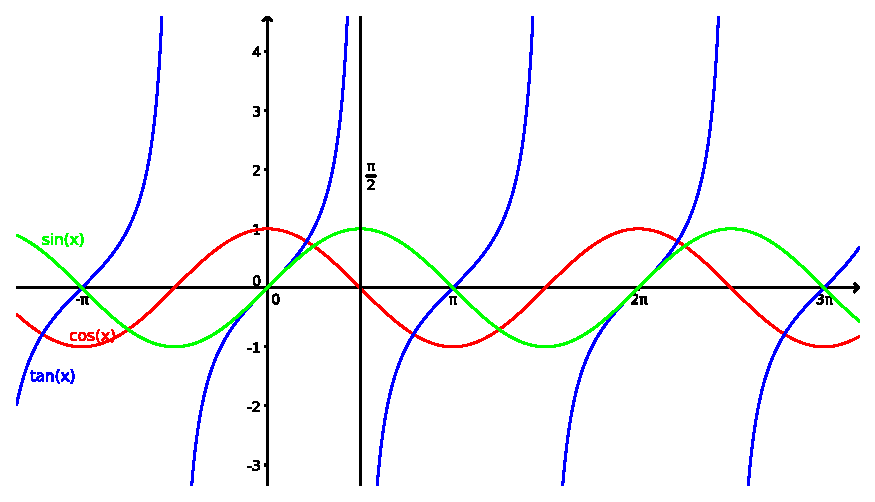
\includegraphics[width=\columnwidth]{sin_cos_tan.eps}

% sinh cosh tanh
% 2 columns (don't insert a new linew between minipage definition, otherwise the layout will break!)
% In order to place the text on top/middle of column next to the image \vspace{0pt} must be inserted!
% Otherwise the text will appear on bottom! Go figure..
\begin{minipage}{0.25\textwidth}
	\vspace{0pt}
	{\footnotesize
	\begin{tabular}{|l||c|c|c|c|c||c|c|}\hline
		 & 0 & $\frac{1}{2}$ & $\frac{\sqrt{2}}{2}$ & $\frac{\sqrt{3}}{2}$ & 1 & DB & WB\\ \hline
		$\arcsin$ & 0 & $\frac{\pi}{6}$ & $\frac{\pi}{4}$ & $\frac{\pi}{3}$ & $\frac{\pi}{2}$ & 
		$[-1, 1]$ & $[-\frac{\pi}{2}, \frac{\pi}{2}]$\\ \hline 

		$\arccos$ & $\frac{\pi}{2}$ & $\frac{\pi}{3}$ & $\frac{\pi}{4}$ & $\frac{\pi}{6}$ & $0$ & 
		$[-1, 1]$ & $[0, \pi]$\\ \hline 

		$\arctan$ & $0$ & - & - & - & $\frac{\pi}{4}$ & $\R$ & $]- \frac{\pi}{2}, \frac{\pi}{2}[$\\ \hline 

		$\sinh$ & 0 & - & - & - & - & $\R$ & $\R$\\ \hline
		$\cosh$ & 1 & - & - & - & - & $\R$ & $[1, \infty[$\\ \hline
		$\tanh$ & 0 & - & - & - & - & $\R$ & $]-1, 1[$\\ \hline
	\end{tabular}
	}
\end{minipage}
\begin{minipage}{0.25\textwidth}
		\vspace{0pt}
		\hspace{1.05cm}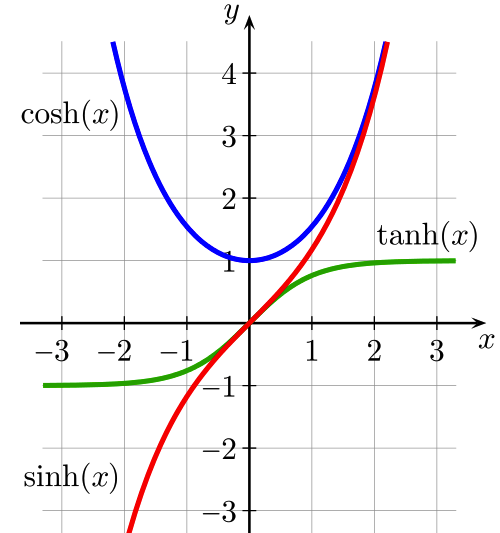
\includegraphics[scale=0.22]{sinh_cosh_tanh_big.png}
\end{minipage}


\subsubsection{Einheitskreis}
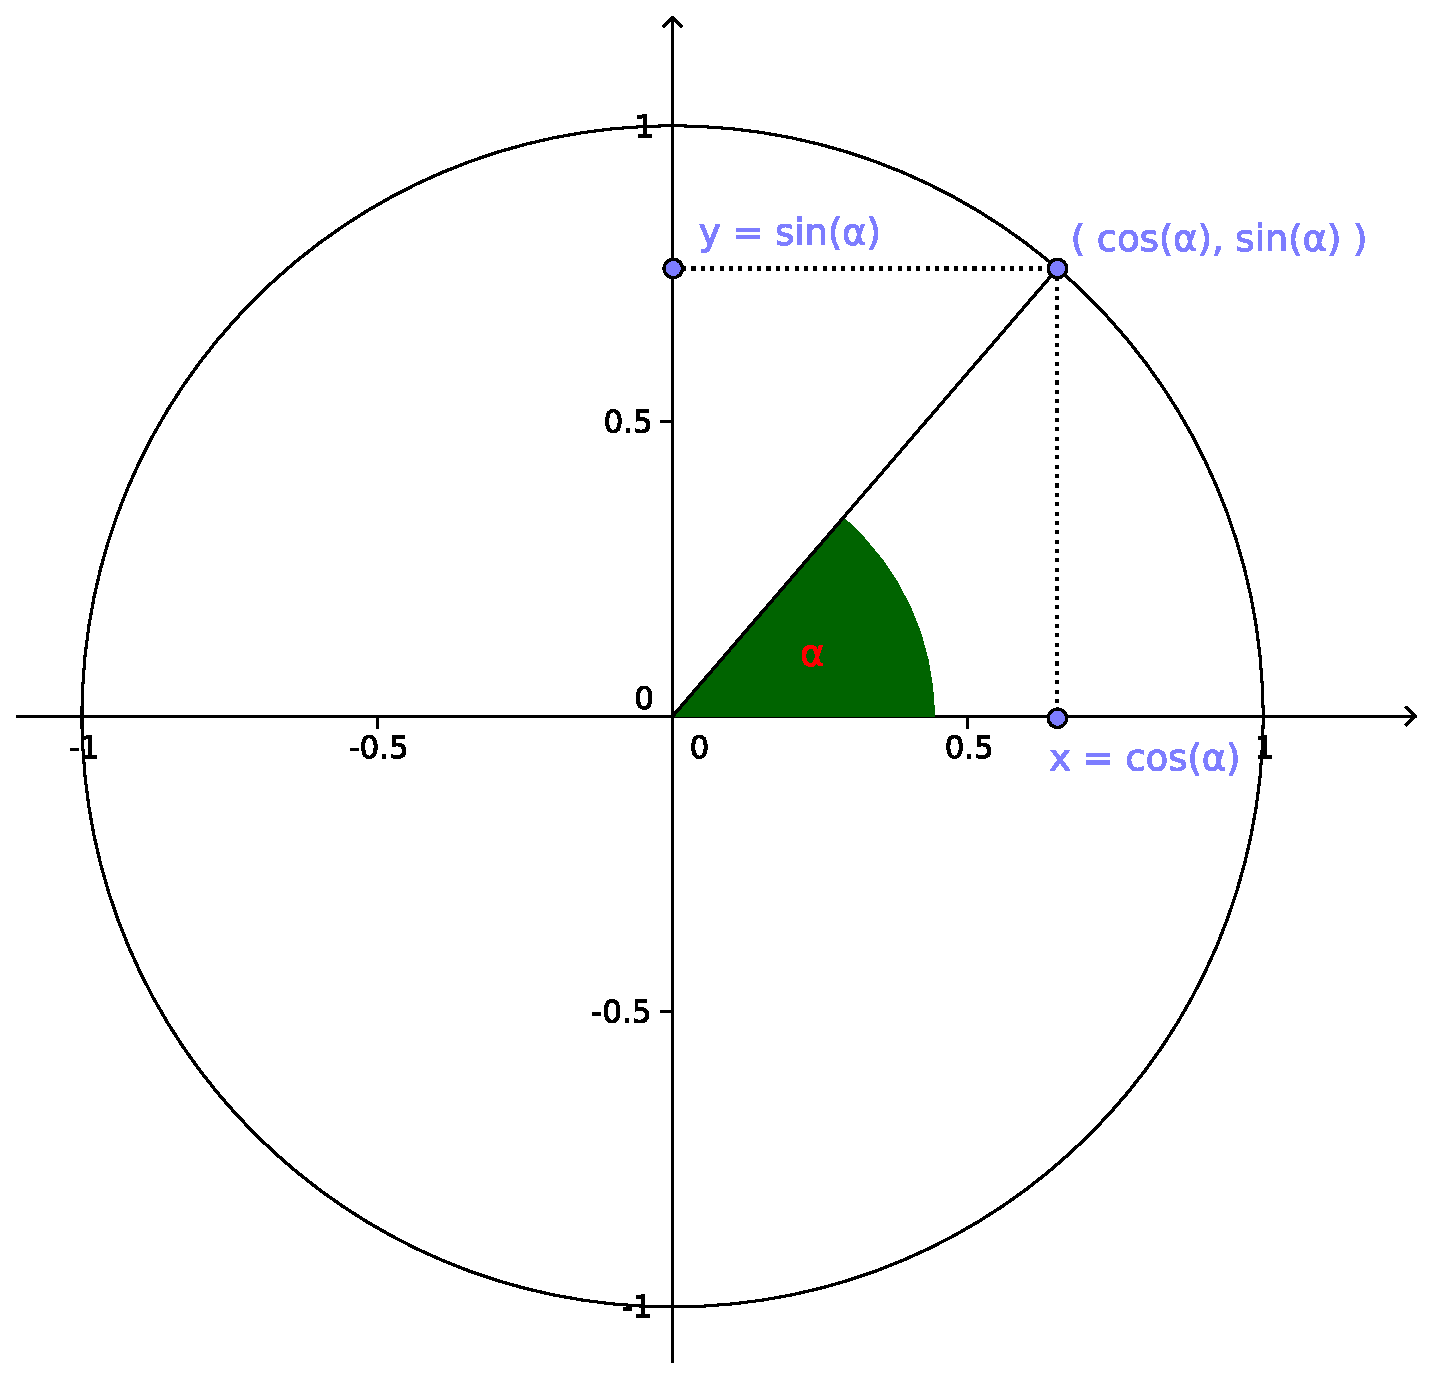
\includegraphics[width=\columnwidth]{einheitskreis_sin_cos.eps}
$\tan \alpha = \frac{\sin \alpha}{\cos \alpha} = \frac{y}{x}$
\pagebreak

\subsection{Trigonom. Funktionen \& Additionstheoreme}
\begin{itemize}[leftmargin=*]
	\item $\sin^2(x) + \cos^2(x) = 1$
	
	% sinus equations
	\item $\sin(90^\circ \pm \alpha) = \cos(\alpha)$
	\item $\sin(180^\circ \pm \alpha) = \mp \sin(\alpha)$
	\item $\sin(\alpha \pm \beta) = \sin(\alpha)\cos(\beta) \pm	\cos(\alpha)\sin(\beta)$
	\item $\sin(2\alpha) = 2 \sin(\alpha)\cos(\alpha)$
	\item $\sin(\alpha)^2 = \frac{1}{2} (1 - \cos(2\alpha))$

	% cosinus equations
	\item $\cos(90^\circ \pm \alpha) = \mp \sin(\alpha)$
	\item $\cos(180^\circ \pm \alpha) = - \cos(\alpha)$
	\item $\cos(\alpha \pm \beta) = \cos(\alpha)\cos(\beta) \mp \sin(\alpha) \sin(\beta)$
	\item $\cos(2\alpha) = \cos^2(\alpha) - \sin^2(\alpha) = 2 \cos^2(\alpha) - 1 = 1 - 2 \sin^2(\alpha)$
	\item $\cos(\alpha)^2 = \frac{1}{2} (1 + \cos(2\alpha))$
	\item $\frac{1}{\cos^2(\alpha)} = 1 + \tan^2(\alpha)$

	% tangens equations
	\item $\tan(\alpha \pm \beta) = \frac{\tan(\alpha) \pm \tan(\beta)}{1 \mp \tan(\alpha)\tan(\beta)}$
	\item $\tan(2\alpha) = \frac{2 \tan(\alpha)}{1 - \tan^2(\alpha)}$
	\item $\tan(\alpha) = \frac{\sin(\alpha)}{\cos{(\alpha)}}$
\end{itemize}

\subsection{Hyperbelfunktionen}
\begin{itemize}[leftmargin=*]
	\item $\sinh(x) = \frac{1}{2}(e^x - e^{-x})$
	\item $\sinh(2x) = 2 \sinh(x) \cosh(x)$
	\item $\sinh(x)^2 = \frac{1}{2} (\cosh(2x) - 1)$
	\item $1 + \sinh(x)^2 = \cosh(x)^2$ $\Leftrightarrow$ $\sqrt{1 + \sinh(x)^2} = \cosh(x)$
	\item $\cosh(x)^2 - \sinh(x)^2 = 1$
	\item $\cosh(x) = \frac{1}{2}(e^x + e^{-x})$
	\item $\cosh(x)^2 = \frac{1}{2} (\cosh(2x) + 1)$
	\item $\tanh(x) = \frac{\sinh(x)}{\cosh(x)} = \frac{e^x - e^{-x}}{e^x +
	e^{-x}} = \frac{e^{2x} - 1}{e^{2x} + 1} = 1 - \frac{2}{e^{2x} + 1}$
	\item $\arcsinh(x) = \ln(x + \sqrt{x^2 + 1})$
	\item $\arcosh(x) = \ln(x + \sqrt{x^2 - 1})$
	\item $\arctanh(x) = \frac{1}{2} \ln(\frac{1+x}{1-x})$
	\item Umformung: $\tanh(x) + 1 = \frac{e^{2x} - 1}{e^{2x} + 1} + 1 = \frac{2x -
	1 + e^{2x} + 1}{e^{2x} + 1} = \frac{2e^{2x}}{e^{2x} + 1}$
\end{itemize}


\subsection{Ableitungen}
{\small
\begin{itemize}[leftmargin=*]
	\item (Summenregel) $(f + g)'(x) = f'(x) + g'(x)$
	\item (Produktregel) $(fg)'(x) = f'(x) \cdot g(x) + f(x) \cdot g'(x)$
	\item (Quotientenregel) $(\frac{f}{g})'(x) = \frac{f'(x) \cdot g(x) -
	f(x) \cdot g'(x)}{g^2(x)}$
	\item (Kettenregel) $(g \circ f)'(x) = (g(f(x)))' = g'(f(x)) \cdot f'(x)$
\end{itemize}}

\subsubsection{Ableitungs-Tafel}
\begin{itemize}[leftmargin=*]
	\item $\frac{d}{dx}\; x^n = nx^{n-1}$
	\item $\frac{d}{dx}\; \frac{1}{x^n} = -n \frac{1}{x^{n+1}}$
	
	% sqrt
	\item 
	\begin{minipage}{0.4\columnwidth}
		$\frac{d}{dx}\; \sqrt{x} = \frac{1}{2\sqrt{x}}$
	\end{minipage}
	\begin{minipage}{0.55\columnwidth}
		$\frac{d}{dx}\; \sqrt[n]{x} = \frac{1}{n\sqrt[n]{x^{n-1}}}$
	\end{minipage}
	
	% e^x
	\item
	\begin{minipage}{0.4\columnwidth}
		$\frac{d}{dx}\; e^x = e^x$
	\end{minipage}
	\begin{minipage}{0.55\columnwidth}
		$\frac{d}{dx}\; e^{\alpha x + \beta} = \alpha e^{\alpha x + \beta}$
	\end{minipage}
	
	\item $\frac{d}{dx}\; e^{x^\alpha} = \alpha x^{\alpha - 1} e^{x^\alpha}$


	\item $\frac{d}{dx}\; \ln(x) = \frac{1}{x}$
	\item $\frac{d}{dx}\; \alpha^x = \alpha^x \ln(\alpha)$
	\item $\frac{d}{dx}\; x^x = x^x (1 + \ln(x))$
	\item $\frac{d}{dx}\; x^{x^\alpha} = x^{x^\alpha + \alpha - 1} (\alpha \log(x) + 1)$ 
	\vspace{0.1cm}\hrule

	% sin cos tan
	\item 
	\begin{minipage}{0.4\columnwidth}
		$\frac{d}{dx}\; \sin(x) = \cos(x)$	
	\end{minipage}
	\begin{minipage}{0.55\columnwidth}
		$\frac{d}{dx}\; \sin(\alpha x + \beta) = \alpha \cos(\alpha x + \beta)$	
	\end{minipage}
	
	
	\item 
	\begin{minipage}{0.4\columnwidth}
		$\frac{d}{dx}\; \cos(x) = -\sin(x)$
	\end{minipage}
	\begin{minipage}{0.55\columnwidth}
		$\frac{d}{dx}\; \cos(\alpha x + \beta) = -\alpha \sin(\alpha x + \beta)$
	\end{minipage}

	\item 
	\begin{minipage}{0.4\columnwidth}
		$\frac{d}{dx}\; \tan(x) = \frac{1}{cos^2(x)}$	
	\end{minipage}
	\begin{minipage}{0.55\columnwidth}
		$\frac{d}{dx}\; \tan(\alpha x + \beta) = \alpha \frac{1}{\cos^2(\alpha x + \beta)}$	
	\end{minipage}
	
	\item $\frac{d}{dx}\; \tan(x) = 1 + \tan(x)^2$

	\item 
	\begin{minipage}{0.4\columnwidth}
		$\frac{d}{dx}\; \arcsin(x) = \frac{1}{\sqrt{1-x^2}}$	
	\end{minipage}
	\begin{minipage}{0.55\columnwidth}
		$\frac{d}{dx}\; \arcsin(\alpha x + \beta) = \frac{\alpha}{\sqrt{1-(\alpha x + \beta)^2}}$
	\end{minipage}
		
	\item 
	\begin{minipage}{0.4\columnwidth}
		$\frac{d}{dx}\; \arccos(x) = -\frac{1}{\sqrt{1-x^2}}$ 
	\end{minipage}
	\begin{minipage}{0.55\columnwidth}
		$\frac{d}{dx}\; \arccos(\alpha x + \beta) = -\frac{\alpha}{\sqrt{1 - (\alpha x + \beta)^2}}$
	\end{minipage}
	
	\item 
	\begin{minipage}{0.4\columnwidth}
		$\frac{d}{dx}\; \arctan(x) = \frac{1}{x^2+1}$
	\end{minipage}
	\begin{minipage}{0.55\columnwidth}
		$\frac{d}{dx}\; \arctan(\alpha x + \beta) = \frac{\alpha}{(\alpha x + \beta)^2 + 1}$
	\end{minipage}
	\vspace{-0.2cm}
	\hrule
	\item 
	{\small
	\begin{minipage}{0.4\columnwidth}
		$\frac{d}{dx}\; \sinh(x) = \cosh(x)$
	\end{minipage}
	\begin{minipage}{0.55\columnwidth}
		$\frac{d}{dx}\; \sinh(\alpha x + \beta) = \alpha \cosh(\alpha x + \beta)$
	\end{minipage}}

	\item
	{\small
	\begin{minipage}{0.4\columnwidth}
		$\frac{d}{dx}\; \cosh(x) = \sinh(x)$
	\end{minipage}
	\begin{minipage}{0.55\columnwidth}
		$\frac{d}{dx}\; \cosh(\alpha x + \beta) = \alpha \sinh(\alpha x + \beta)$
	\end{minipage}}
	
	\item 
	{\small
	\begin{minipage}{0.4\columnwidth}
		$\frac{d}{dx}\; \tanh(x) = \frac{1}{\cosh^2(x)}$
	\end{minipage}
	\begin{minipage}{0.55\columnwidth}
		$\frac{d}{dx}\; \tanh(\alpha x + \beta) = \alpha \frac{1}{\cosh^2(\alpha x + \beta)}$
	\end{minipage}}

	\item 
	{\small
	\begin{minipage}{0.4\columnwidth}
		$\frac{d}{dx}\; \arcsinh(x) = \frac{1}{\sqrt{x^2 + 1}}$
	\end{minipage}
	\begin{minipage}{0.55\columnwidth}
		$\frac{d}{dx}\; \arcsinh(\alpha x + \beta) = \frac{\alpha}{\sqrt{(\alpha x + \beta)^2 + 1}}$
	\end{minipage}}
	
	\item
	{\footnotesize
	\begin{minipage}{0.4\columnwidth}
		$\frac{d}{dx}\; \arcosh(x) = \frac{1}{\sqrt{x-1} \sqrt{x + 1}}$
	\end{minipage}
	\begin{minipage}{0.55\columnwidth}
		$\frac{d}{dx}\; \arcosh(\alpha x + \beta) = \frac{\alpha}{\sqrt{\alpha x + \beta - 1} \sqrt{\alpha x + \beta + 1}}$
	\end{minipage}}

	\item 
	{\small
	\begin{minipage}{0.4\columnwidth}
		$\frac{d}{dx}\; \arctanh(x) = \frac{1}{1-x^2}$
	\end{minipage}
	\begin{minipage}{0.55\columnwidth}
		$\frac{d}{dx}\; \arctanh(\alpha x + \beta) = \frac{\alpha}{1 - (\alpha x + \beta)^2}$
	\end{minipage}}
\end{itemize}

\subsection{Integrale}
\subsubsection{Integralregeln}
\begin{itemize}[leftmargin=*]
	\item $\int u'\cdot v \, dx = uv - \int u \cdot v' \, dx$
	\item $\int \frac{f'(x)}{f(x)} \, dx = \ln|f(x)|$
	\item $\int f(x)f'(x) \, dx = \frac{1}{2}f(x)^2$
	\item $|\int f(x)| \leq \int |f(x)|$ (wenn f, Riemann-Integrable ist)
\end{itemize}

\subsubsection{typische Integrale}
\begin{itemize}[leftmargin=*]
	% typ: x^n
	\item $\int x^n \, dx = \frac{x^{n+1}}{n+1}$ \hspace{0.3cm} für $n \neq -1$
  	\item $\int(ax + b)^n \,dx = \frac{(ax + b)^{n+1}}{(n + 1)a}$ \hspace{0.3cm} für $n \neq -1$
	\item $\int x(ax+b)^n \,dx = \frac{(ax + b)^{n+2}}{(n+2)a^2} - \frac{b(ax+b)^{n+1}}{(n+1)a^2}$

  	% typ: 1/x resulting in ln
  	\item $\int \frac{1}{x} \,dx = \ln |x|$
	\item $\int \frac{1}{x^2} \,dx = -\frac{1}{x}$
  	\item $\int \frac{1}{a+x} \,dx = \ln |a+x|$
  	\item $\int \frac{1}{(a+x)^2} \,dx = - \frac{1}{a+x}$
	\item $\int \frac{1}{ax+b} \,dx = \frac{1}{a} \ln |ax+b|$
	\item $\int \frac{x}{1 + x^2} \, dx = \frac{1}{2} \ln |1 + x^2|$

	% typ: 1/x resulting in arctan
	\item $\int \frac{1}{1 + x^2} \, dx = \arctan(x)$
	\item $\int \frac{1}{a^2 + x^2} \,dx = \frac{1}{a} \arctan(\frac{x}{a})$
	\item $\int \frac{1}{a^2 - x^2} \,dx = \frac{1}{a} \arctanh(\frac{x}{a})$
	\item $\int \frac{1}{1 + (a + x)^2} \, dx = \arctan(a + x)$
	
	
	% typ: ln
  	\item $\int \ln(x) \,dx = x(\ln(x) - 1)$
  	\item $\int \ln(ax + b) \,dx = \frac{(a x+b) \ln (a x+b)-a x}{a}$
	
	% typ: sqrt
	\item $\int \sqrt{x} \,dx = \frac{2}{3}\sqrt{x^3}$
	\item $\int \frac{1}{\sqrt{x}} \,dx = 2 \sqrt{x}$	
	%mühsamer kerl der teilweise in prüfungen verwendet wird. Kann man über subsitution von x mit sin(u) lösen.
	\item $\int \sqrt{1-x^2} \,dx = \frac{1}{2}\left( x\sqrt{1-x^2}+ \arcsin(x) \right)$
	\item $\int \frac{1}{\sqrt{1 - x^2}} \, dx = \arcsin(x)$
	\item $\int \frac{1}{\sqrt{1 + x^2}} \, dx = \arcsinh(x)$

	\item $\int a^{xb + c} \,dx = \frac{a^{bx + c}}{b \log(a)}$
	\item $\int \frac{ax + b}{px + q} \,dx = \frac{ax}{p} + \frac{bp - aq}{p^2} \ln |pq+q|$
\end{itemize}

\subsubsection{trionometrische Funktionen}
\begin{itemize}[leftmargin=*]
	% sin
	\item
	\begin{minipage}{0.5\columnwidth}
		$\int \sin(x) \, dx = - \cos(x)$
	\end{minipage}
	\begin{minipage}{0.45\columnwidth}
		$\int \sin(ax) \,dx = -\frac{1}{a}\cos(ax)$
	\end{minipage}

	\item
	\begin{minipage}{0.5\columnwidth}
		 $\int \sin(x)^2 \, dx = \frac{x}{2} - \frac{\sin(x) \cos(x)}{2}$
	\end{minipage}
	\begin{minipage}{0.45\columnwidth}
		$\int \sin(ax)^2 \,dx = \frac{x}{2} - \frac{sin(2ax)}{4a}$
	\end{minipage}
		  
	\item $\int x \sin(ax) \,dx = \frac{\sin(ax)}{a^2} - \frac{x \cos(ax)}{a}$
	\item $\int \frac{1}{\sin^2 x} \,dx = -\cot x$
   	\item $\int \sin(ax) \cos(ax) \,dx = -\frac{\cos^2(ax)}{2a}$

   	% cos
   	\item 
	\begin{minipage}{0.5\columnwidth}
		$\int \cos(x) \, dx = \sin(x)$
	\end{minipage}
	\begin{minipage}{0.45\columnwidth}
		$\int \cos(ax) \,dx = \frac{1}{a}\sin(ax)$
	\end{minipage}

	\item
	\begin{minipage}{0.5\columnwidth}
		$\int \cos(x)^2 \, dx = \frac{x}{2} + \frac{\sin(x) \cos(x)}{2}$
	\end{minipage}
	\begin{minipage}{0.45\columnwidth}
		$\int \cos^2(ax) \,dx = \frac{x}{2} + \frac{\sin(2ax)}{4a}$
	\end{minipage}
		  
	\item $\int \cos(ax) \,dx = \frac{\cos(ax)}{a^2} + \frac{x \sin(ax)}{a}$
	\item $\int \frac{1}{\cos^2(x)} \,dx = \tan x$
	
	% rest
	\item $\int \tan(ax) \,dx = - \frac{1}{a} \ln | \cos(ax) |$
	\item $\int \arcsin(x) \,dx = x \arcsin(x) + \sqrt{1 - x^2}$
	\item $\int \arccos(x) \,dx = x \arccos(x) - \sqrt(1-x^2)$
	\item $\int \arctan(x) \,dx = x \arctan(x) - \frac{1}{2} \ln(1+x^2)$
\end{itemize}

\subsubsection{Hyperbelfunktionen}
\begin{itemize}[leftmargin=*]
	\item 
	\begin{minipage}{0.43\columnwidth}
		$\int \sinh(x) \,dx = \cosh(x)$
	\end{minipage}
	\begin{minipage}{0.52\columnwidth}
		$\int \sinh(ax + b) \,dx = \frac{\cosh(ax + b)}{a}$
	\end{minipage}

	\item
	\begin{minipage}{0.43\columnwidth}
		$\int \cosh(x) \,dx = \sinh(x)$
	\end{minipage}
	\begin{minipage}{0.52\columnwidth}
		$\int \cosh(ax + b) \,dx = \frac{\sinh(ax + b)}{a}$
	\end{minipage}
	
	\item
	\begin{minipage}{0.43\columnwidth}
		$\int \tan(x) \,dx = \log(\cosh(x))$
	\end{minipage}
	\begin{minipage}{0.52\columnwidth}
		$\int \tan(ax + b) \,dx = \frac{\log(\cosh(ax+b))}{a}$
	\end{minipage}
\end{itemize}

\subsubsection{Exponentialfunktion}
\begin{itemize}[leftmargin=*]
  	\item $\int e^{ax} \,dx = \frac{1}{a} e^{ax}$ 
	\item $\int x e^{ax} \,dx = e^{ax} \cdot \left ( \frac{ax - 1}{a^2} \right )$
	\item $\int x \ln(x) \,dx = \frac{1}{2} x^2 (\ln(x) - \frac{1}{2})$
	\item $\int_{-\infty}^\infty e^{-\frac{1}{a}x^2} \,dx = \sqrt{a \pi}$
\end{itemize}
\pagebreak
\subsection{Reihenentwicklung}
\begin{itemize}[leftmargin=*]
	\item $e^x = \sum_{n=0}^\infty \frac{x^n}{n!} = 1 + \frac{x}{1!} + \frac{x^2}{2!} + \frac{x^3}{3!} + 
				 \frac{x^4}{4!} + \cdots$
	\item $\sin x = \sum_{n=0}^\infty (-1)^n \frac{x^{2n + 1}}{(2n + 1)!} = x - \frac{x^3}{3!} + \frac{x^5}{5!} + \cdots$
	\item $\cos x = \sum_{n=0}^\infty (-1)^n \frac{x^{2n}}{(2n)!} = 1 - \frac{x^2}{2!} + \frac{x^4}{4!} - \cdots + \cdots$
	\item $\sinh x = \sum_{n=0}^\infty \frac{x^{2n+1}}{(2n + 1)!}$
	\item $\cosh x = \sum_{n=0}^\infty \frac{x^{2n}}{(2n)!}$
	\item $\ln x = \sum_{n=0}^\infty \frac{2}{2n + 1} \cdot \left(\frac{x-1}{x+1} \right)^{2n}$
\end{itemize}

\subsection{Grenzwerte}
\begin{itemize}[leftmargin=*]
	\item \textbf{Bernoullische Ungleich.}: $x \geq -1, n \in \N: \; (1+x)^n \geq 1+nx$
	\item \textbf{Vergleich von Folgen}: weiter rechts stehende Folgen streben
	schneller gegen $\infty$:
	\[
		1, \quad \ln n, \quad n^\alpha (\alpha > 0), \quad q^n (q > 1), \quad n!, \quad n^n \Rightarrow
		\lim_{x \to \infty} \frac{\ln n}{n^\alpha} = 0
	\]
\end{itemize}
$\lim_{n \to \infty}$
\begin{itemize}[leftmargin=*]
	\item $\lim_{n \to \infty} \sqrt[n]{a} \rightarrow 1$
	\item $\lim_{n \to \infty} \sqrt[n]{n} \rightarrow 1$
	\item $\lim_{n \to \infty} \sqrt[n]{n!} \rightarrow \infty$
	\item $\lim_{n \to \infty} \frac{n}{\sqrt[n]{n!}} \rightarrow e$
	\item $\lim_{n \to \infty} \frac{1}{n} \sqrt[n]{n!} \rightarrow \frac{1}{e}$
	\item $\lim_{n \to \infty} \left ( \frac{n+1}{n} \right )^n \rightarrow e$
	\item $\lim_{n \to \infty} \left ( 1 + \frac{1}{n} \right )^n \rightarrow e$
	\item $\lim_{n \to \infty} \left ( 1 - \frac{1}{n} \right )^n \rightarrow \frac{1}{e}$
	\item $\lim_{n \to \infty} \left ( \frac{n}{1 + n} \right )^n \rightarrow \frac{1}{e}$
	\item $\lim_{n \to \infty} \left ( 1 + \frac{x}{n} \right )^n \rightarrow e^x$
	\item $\lim_{n \to \infty} \left ( 1 - \frac{x}{n} \right )^n \rightarrow \frac{1}{e^x}$
	\item $\lim_{n \to \infty} {a \choose n} \rightarrow 0, \; a > -1$
	\item $\lim_{n \to \infty} \frac{a^n}{n!} \rightarrow 0$
	\item $\lim_{n \to \infty} \frac{n^n}{n!} \rightarrow \infty$
	\item $\lim_{n \to \infty} \frac{a^n}{n^k} \rightarrow \infty, a > 1, k$ fest
	\item $\lim_{n \to \infty} a^n n^k \rightarrow 0, |a| < 1, k$ fest
	\item $\lim_{n \to \infty} n(\sqrt[n]{a} - 1) \rightarrow \ln a, a > 0$
	\item $\lim_{n \to \infty} \left( 1+\frac{x}{n} \right)^n = e^x \quad$
	\item $\lim_{n \to \infty} \sqrt[n]{n} = 1$
	\item $\lim_{n \to \infty} n^p q^n = 0 \qquad p \in \N \text{ und } 0 < q < 1$
	\item $\lim_{x \to \infty} \sqrt{x^2-x}-x = \frac{1}{2}$ 
	%\newline
	%{\small (Lösungsansatz mit Taylorreihe
	%($\sqrt{1-x} = 1 + \frac{x}{2}+O(x^2)$): $\sqrt{x^2-x}-x = x(\sqrt{1-\frac{1}{x}}-1) =
	%x((1+\frac{1}{2x}+O(\frac{1}{x^2}))-1) = \frac{1}{2}+O(\frac{1}{x}) \underset{n \to \infty}{\longrightarrow} \frac{1}{2}$ )}
\end{itemize}
$\lim_{x \to 0}$
\begin{itemize}[leftmargin=*]
	\item $\lim_{x \to 0} \frac{a^x - 1}{x} = \ln a$
	\item $\lim_{x \to 0} \frac{\sin x}{x} = 1$
	\item $\lim_{x \to 0} \left| \frac{\cos x}{x} \right| = +\infty$
	\item $\lim_{x \to 0} \frac{1 - \cos x}{x} = 0$
	\item $\lim_{x \to 0} \frac{1 - \cos x}{x^2} = \frac{1}{2}$
	\item $\lim_{x \to 0} \frac{\tan x}{x} = 1$
	\item $\lim_{x \to 0} \frac{\log_a (1 + x)}{x} = \frac{1}{\ln a}$
	\item $\lim_{x \to 0} x^a \ln x = 0, \; a  > 0$
\end{itemize}

\subsection{Reihen}
\begin{itemize}[leftmargin=*]
	\item
	\begin{minipage}{0.35\columnwidth}
		$\sum_{n=1}^\infty \frac{1}{n}$
	\end{minipage}
	\begin{minipage}{0.60\columnwidth}
		divergiert (``harmonische Reihe'')
	\end{minipage}

	\item $\sum_{n=1}^\infty \frac{(-1)^n}{n} = \ln \frac{1}{2}$
	\item 
	\begin{minipage}{0.35\columnwidth}
		$\sum_{n=1}^\infty \frac{1}{n^\alpha}$
	\end{minipage}
	\begin{minipage}{0.60\columnwidth}
		konver. für $\alpha > 1$, divergiert für $\alpha \leq 1$
	\end{minipage}
	 
	\item 
	\begin{minipage}{0.35\columnwidth}
		$\sum_{n=0}^\infty q^n = \frac{1}{1-q}$
	\end{minipage}
	\begin{minipage}{0.60\columnwidth}
		für $|q| < 1$ (``geometrische Reihe'')
	\end{minipage}
	
	\item
	\begin{minipage}{0.35\columnwidth}
		$\sum_{n=0}^\infty (-1)^n q^n = \frac{1}{1-q}$
	\end{minipage}
	\begin{minipage}{0.60\columnwidth}
		für $|q| < 1$ (``geometrische Reihe'')
	\end{minipage}

	\item $\sum_{n=1}^\infty \frac{1}{n^2} = \frac{\pi^2}{6}$
	\newline
	\item $\sum_{n=0}^m q^n = \frac{1-q^{m+1}}{1-q}$ 
	\item $\sum_{n=1}^m n = \frac{m(m+1)}{2}$
	\item  $\sum_{n=0}^m n^2 = \frac{1}{6}m(m+1)(2m+1)$
	\item  $\sum_{n=0}^m n^3 = \frac{1}{4}m^2(m+1)^2$
\end{itemize}

\subsection{Linienintegral}
\begin{itemize}[leftmargin=*]
	\item 2. Art: $\int_\gamma \vec{f}(\vec{x}) d\vec{x} := \int_a^b \left<
	\vec{f}(\gamma(t)), \gamma(t)' \right>\; dt$
	\item 1. Art: $\int_\gamma f ds := \int_a^b f(\gamma(t)) \|\gamma(t)'\|_2\; dt$
\end{itemize}

\subsection{Kreuzprodukt}
{\footnotesize
\[
\vec{a} \times \vec{b} = \left ( \begin{array}{c} a_1 \\ a_2 \\ a_3 \end{array}
\right ) \times
\left ( \begin{array}{c} b_1 \\ b_2 \\ b_3 \end{array}
\right ) =
\left ( \begin{array}{c} a_2b_3 - a_3b_2 \\ a_3b_1 - a_1b_3 \\ a_1b_2 - a_2b_1
\end{array} \right )
\]
}

\begin{multicols}{2}
\subsection{Exponent}
\begin{itemize}[leftmargin=*]
  \item $a^n a^m = a^{n + m}$
  \item $\frac{a^n}{a^m} = a^{n - m}$
  \item $(a^n)^m = a^{nm}$
  \item $(ab)^n = a^n b^n$
  \item $\left( \frac{a}{b} \right)^n = \frac{a^n}{b^n}$
  \item $a^{-n} = \frac{1}{a^n}$
  \item $\left( \frac{a}{b} \right)^{-n} = \left( \frac{b}{a} \right)^n$
  \item $a^\frac{n}{m} = (a^\frac{1}{m})^n = (a^n)^\frac{1}{m}$
  \item $a^{n^m} = a^{(n^m)}$
\end{itemize}
\columnbreak

\subsection{Wurzel}
\begin{itemize}[leftmargin=*]
  \item $\sqrt[n]{a} = a^\frac{1}{n}$
  \item $\sqrt[n]{ab} = \sqrt[n]{a} \sqrt[n]{b}$
  \item $\sqrt[m]{\sqrt[n]{a}} = \sqrt[nm]{a}$
  \item $\sqrt[n]{\frac{a}{b}} = \frac{\sqrt[n]{a}}{\sqrt[n]{b}}$
\end{itemize}

\end{multicols}

\subsection{Ungleichungen}
\begin{itemize}[leftmargin=*]
  \item $a < b \Rightarrow a + c < b + c$ und $a - c < b - c$
  \item $a < b$ und $c > 0 \Rightarrow \frac{a}{c} < \frac{b}{c}$
  \item $a < b$ und $c < 0 \Rightarrow \frac{a}{c} > \frac{b}{c}$ 
  \item Dreiecksungleichung für reelle Zahlen: $|a+b| \le |a|{+}|b|$ %Quelle Wikipedia: http://de.wikipedia.org/wiki/Dreiecksungleichung#Dreiecksungleichung_f.C3.BCr_reelle_Zahlen
  \item Cauchy-Schwarz Ungleichung: $|x \cdot y| \leq \|x\| \cdot \|y\|, \; x,y \in \R^n$
\end{itemize}

\subsection{Logarithmen}
\begin{itemize}[leftmargin=*]
  \item $y = \log_a x \Leftrightarrow x = a^y$
  \item $\log_a 1 = 0$
  \item $\log_a a^x = x$
  \item $a^{\log_a x} = x $
  \item $\log_a x \cdot y = \log_a x + \log_a y$
  \item $\log_a \frac{x}{y} = \log_a x - \log_a y$
  \item $\log_a \frac{1}{x} = - \log_a x$
  \item $\log_a x^r = r \log_a x$
  \item $\log_a x = \frac{\log_b x}{\log_b a}$
  \item $\log_a x = \frac{\ln x}{\ln a}$
  \item $\log_a (x+y) = \log_a x + log_a (1 + \frac{y}{x})$
  \item $\log_a (x-y) = \log_a x + \log_a (1- \frac{y}{x})$
\end{itemize}

\subsection{Exponentialfunktion}
\begin{itemize}[leftmargin=*]
  \item $e^{-\inf} = 0$
  \item $e^0 = 1$
  \item $e^1 = e =  2.718281828$
  \item $e^{\inf} = \inf$
  \item $e^{a+bi} = e^a(\cos(b) + i \sin(b))$ (Euler Identität)
  \item $e^{b \ln(a)} = a^b$
  \item $ e^{-\ln(b)} = \frac{1}{b}$ 
\end{itemize}

\subsection{Komplexe Zahlen}
\begin{itemize}[leftmargin=*]
	\item $z \in \C: z = a + b\cdot i$
	\item $\bar{z} = a - b\cdot i$
	\item $|z|^2 = z \cdot \bar{z} = (a + b\cdot i) \cdot (a - b\cdot i) = a^2 + b^2$
	\item $i^2 = -1$
	\item $(a + bi) + (c + di) = (a + c) + (b + d)i$
	\item $(a + bi) \cdot (c + di) = (ac - bd) + (ad + bc)i$
	\item $\frac{a + bi}{c + di} = \frac{ac + bd}{c^2 + d^2} + \frac{bc - ad}{c^2 + d^2}\cdot i$
\end{itemize}
\pagebreak
\subsection{Geometrische Körper}
\subsubsection{Ellipsoid}
Hat die Form eines Rugbyballs. In kartesischen Koordinaten definert durch
$\frac{x^2}{a^2} + \frac{y^2}{b^2} + \frac{z^2}{c^2} - 1 = 0$.

\subsection{Geometrie in 3D}
%evtl. nicht nötig. Aber in alten prüfungen oft gefragt.
\subsubsection*{Masse von speziellen Gebieten}
	\begin{multicols}{2}
	\renewcommand\arraystretch{1.4}
	\begin{tabular}{l|l}
		Zylinder   &   $ V = \pi r^2 h $ \\
		Pyramide   &   $ V = \frac{1}{3} G h $ \\
		Ellipsoid   &   $ V = \frac{4 \pi}{3} a b c $ \\
		Kegel   &   $ V = \frac{\pi}{3} r^2 h $ \\
		Kegelstumpf   &   $ V = \frac{\pi h}{3} (r_1^2+r_2^2 + r_1 r_2) $ 
	\end{tabular}
	
	\columnbreak
	\begin{tabular}{l|l}
		Torus   &   $ V = 2 \pi^2 R r^2 $ \\
		   &   $ S = 4 \pi^2 R r $ \\
		Kugel   &   $ V = \frac{4 \pi}{3} r^3 $ \\
		   &   $ S = 4 \pi r^2 $ 
	\end{tabular}
	\end{multicols}

\subsubsection*{Rotationskörper (Volumen / Mantelfläche)}
Rotation um die x Achse $V =\pi \int_a^b f(x)^2 dx.$\\
Rotation um die x Achse $M = 2\pi \int_a^b f(x) \, \sqrt{1 + f'(x)^2} dx$\\
{\small \textbf{Achtung:} Für ganze Fläche muss Deckel dazu berechnet werden!}
% Rotation um die y Achse $V=2\pi \int_a^b x \cdot f(x) dx$ => falsch!

\subsection{Kosinussatz}
\begin{minipage}{0.35\columnwidth}
	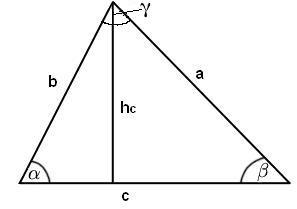
\includegraphics[width=\columnwidth]{kosinussatz.jpg}
\end{minipage}
\begin{minipage}{0.60\columnwidth}
	\begin{eqnarray*}
		a^2 = b^2 + c^2 - 2bc \, \cdot \, \cos(\alpha)\\
		b^2 = a^2 + c^2 - 2ac \, \cdot \, \cos(\beta)\\
		c^2 = a^2 + b^2 - 2ab \, \cdot \, \cos(\gamma)
	\end{eqnarray*}
\end{minipage}

\subsection{Ausklammern}
\begin{itemize}[leftmargin=*]
	\item $x^n - y^n = (x-y) (x^{n-1} + x^{n-2}y + x^{n-3}y^2 + \ldots + xy^{n-2}
	+ y^{n-1})$
	\item $x^n - 1 = (x-1)(x^{n-1} + x^{n-2} + \ldots + x + 1)$
\end{itemize}

\subsection{Aus Serien}
\begin{itemize}[leftmargin=*]
	\item Ableitung von $x^x$ kann man mit Ansatz $x = e^{\log(x)}$ berechnen.
	Also:$ \frac{d}{dx}  e^{\log(x^x)} = \frac{d}{dx} e^{x \log(x)} = x^x (1 + \log(x))$
	\item Euler Identität (komplexe Zahlen): $e^{ix} = \cos(x) + i \sin(x)$
\end{itemize}

\subsection{Polynomdivision}
Zu jedem Zeitpunkt gilt: Zähler : Nenner = Ergebnis, wobei der Zähler und das Ergebnis sich nach einem Schritt jeweils ändern.
\begin{enumerate}[leftmargin=*]
	\item Prüfe ob Grad des Zählers $\geq$ Grad des Nenners ist.
	\begin{enumerate}
		\item Falls Ja:
		\begin{enumerate}
			\item Dividiere höchsten Grad vom Zähler durch höchsten Grad vom Nenner und addiere das Resultat zum Ergebnis.
			\item Multipliziere den neu hinzugefügten Summanden mit dem Nenner und notiere dieses Zwischenresultat. Danach berechne Zähler - Zwischenresultat und betrachte das als neuen Zähler. Starte wieder bei 1.
		\end{enumerate}
		\item Falls Nein:\\
		Wir sind fertig. Wenn noch ein Rest übrig bleibt, muss dies dem Ergebnis noch hinzugefügt werden. Also Rest / Nenner noch dem Erebnis addieren werden. 
	\end{enumerate}
\end{enumerate}
\textbf{Beispiel} \\
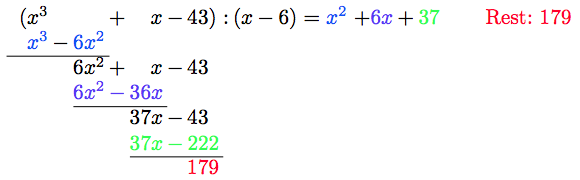
\includegraphics[scale=0.45]{polynomdivision_rechnung.png}
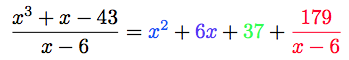
\includegraphics[scale=0.45]{polynomdivision_resultat.png}

\begin{landscape}\begin{multicols}{3}

\subsection{\texorpdfstring{$\log(x)$}{log(x)}}
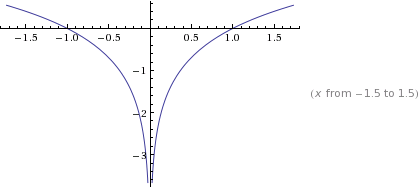
\includegraphics[scale=0.5]{log_x.png}

\subsection{\texorpdfstring{$\frac{1}{x}$}{1/x}}
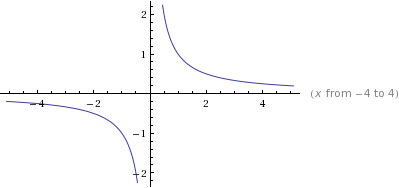
\includegraphics[scale=0.5]{1_over_x.png}

\subsection{\texorpdfstring{$\sqrt{x}$}{x^(1/x)}}
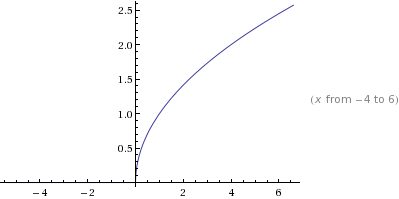
\includegraphics[scale=0.5]{sqrt_x.png}

\subsection{$e^x$}
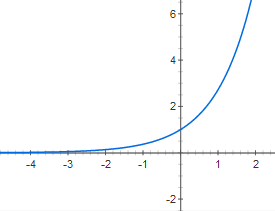
\includegraphics[width=0.5\columnwidth]{e_x}

\subsection{Funktionsmanipulation}
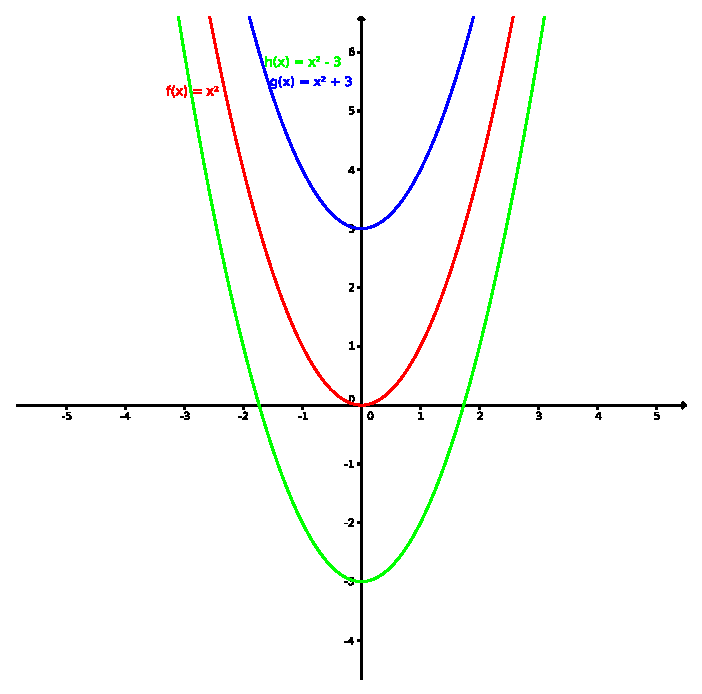
\includegraphics[width=\columnwidth]{manipulation_1.eps}
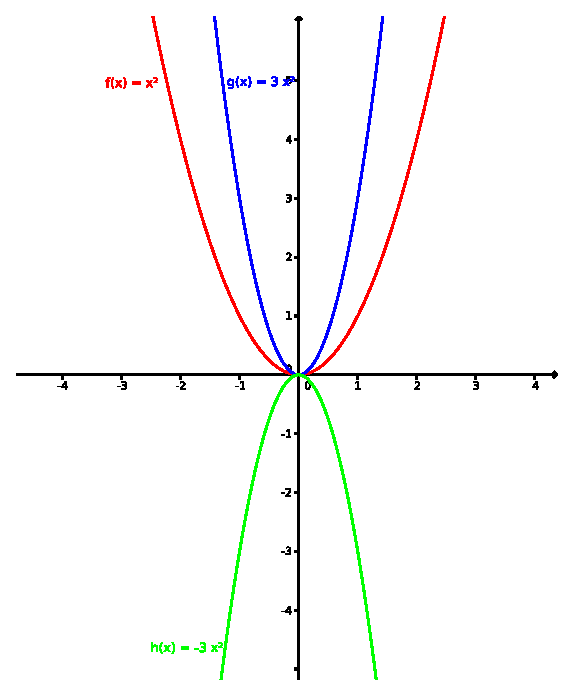
\includegraphics[width=\columnwidth]{manipulation_2.eps}
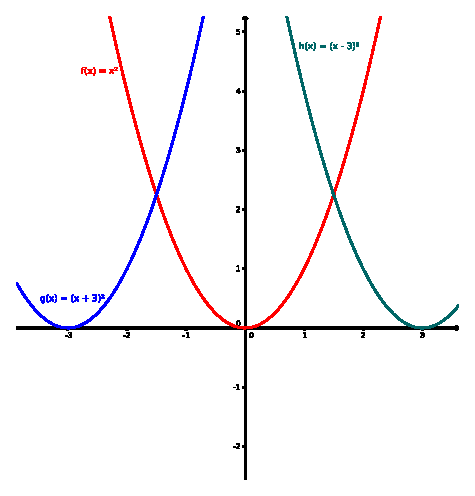
\includegraphics[width=\columnwidth]{manipulation_3.eps}

\subsection{Pascalsches Dreieck}
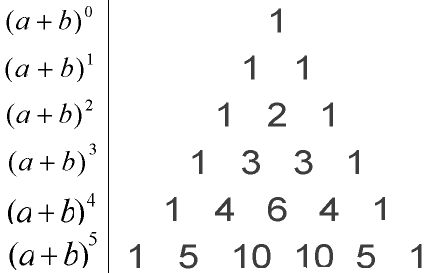
\includegraphics[width=\columnwidth]{pascal.png}

\end{multicols}\end{landscape}

\begin{multicols}{2}
\subsection{$\log(x)$}
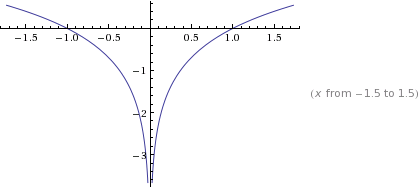
\includegraphics[width=\columnwidth]{log_x.png}

\subsection{$\frac{1}{x}$}
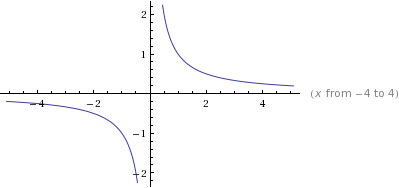
\includegraphics[width=\columnwidth]{1_over_x.png}

\subsection{$\sqrt{x}$}
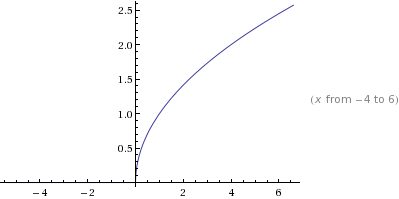
\includegraphics[width=\columnwidth]{sqrt_x.png}

\subsection{$e^x$}
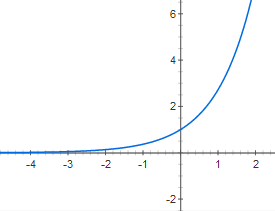
\includegraphics[width=\columnwidth]{e_x}

\subsection{\small $f$ Verschiebungen}
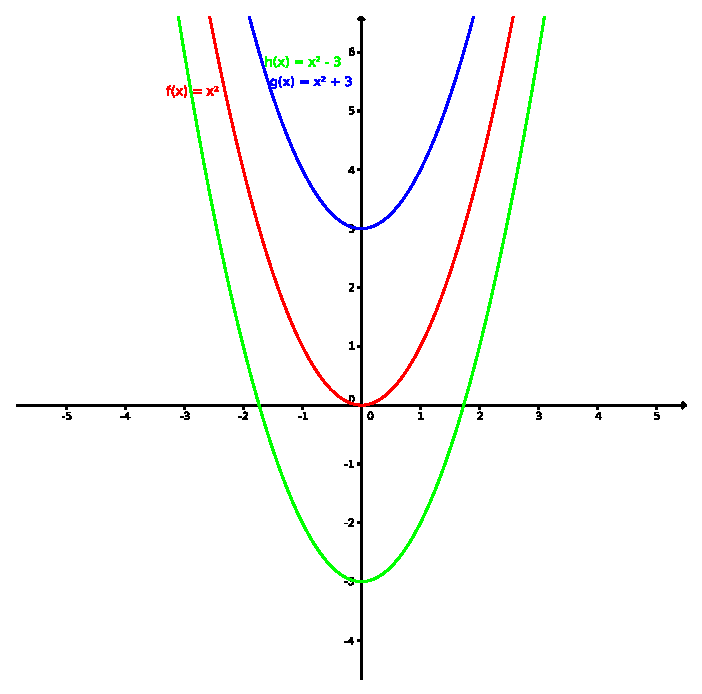
\includegraphics[width=\columnwidth]{manipulation_1.eps}
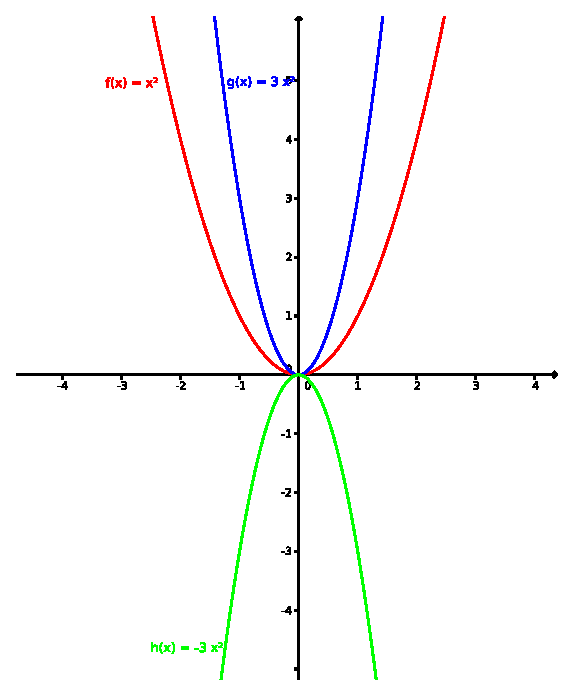
\includegraphics[width=\columnwidth]{manipulation_2.eps}
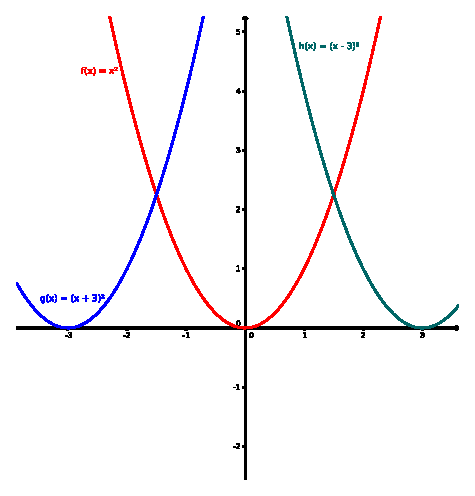
\includegraphics[width=\columnwidth]{manipulation_3.eps}

\subsection{Pascalsches $\Delta$}
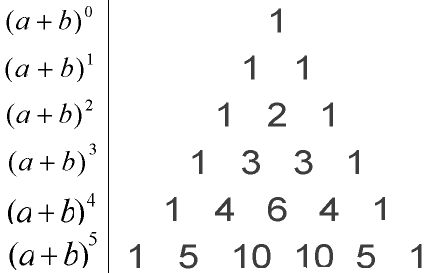
\includegraphics[width=\columnwidth]{pascal.png}
\end{multicols}

% fill the page
\clearpage

\end{document}
